\documentclass[a4paper,14pt]{extarticle}
\usepackage{cmap}				% To be able to copy-paste russian text from pdf			
\usepackage[utf8]{inputenc}
\usepackage[T1]{fontenc}
\usepackage[margin=1in]{geometry}
\usepackage[english, russian]{babel}

\usepackage[hyphens]{url}
\urlstyle{same}
\usepackage{hyperref}

\usepackage{multirow}
\usepackage{graphicx}
\usepackage{caption}
\usepackage{amsmath}
\usepackage{mathtools}

\usepackage{tikz}
\usepackage{pgfplots}
\usepgfplotslibrary{groupplots,colorbrewer,dateplot,statistics}

%\def\ishtml{1}
\ifdefined\ishtml
  % HTML mode
  \newcommand{\urlnote}[2]{\href{#2}{#1}} % Make cool link 
  \newcommand{\smallsep}{thinspace} % to be replaced with unicode 8239 later
\else
  % PDF mode
   \usepackage{libertine}
   \usepackage{libertinust1math}
   \newcommand{\urlnote}[2]{#1\endnote{\url{#2}}}  % Put URLs to endnotes
   \newcommand{\smallsep}{\kern 0.1em}
\fi

% Move footnotes to end of document
\usepackage[backref=true]{enotez}
\DeclareTranslation{russian}{enotez-title}{Примечания}

\usepackage[
	output-decimal-marker={,},
	group-separator={\smallsep},
	group-minimum-digits=3
]{siunitx}

% Shoot me if I know a better way to make decimal groups of two
\newcommand{\rateone}[1]{\num{#1}}
\newcommand{\ratetwo}[2]{\num{#1}\smallsep#2}
\newcommand{\ratethree}[3]{\num{#1}\smallsep#2\smallsep#3}

\newcommand{\ru}[1]{\begin{otherlanguage}{russian}#1\end{otherlanguage}}
\newcommand{\en}[1]{\begin{otherlanguage}{english}#1\end{otherlanguage}}
\newcommand{\ruen}[2]{#1 (\en{#2})}

\usepackage[style=alphabetic, backend=biber]{biblatex}
\addbibresource{index.bib}
\renewcommand*{\bibfont}{\small}
\setcounter{biburllcpenalty}{9000}
\setcounter{biburlucpenalty}{9500}

\author{Артём Бакулин}
\date{\today}
\title{Индексное инвестирование}

\begin{document}

\maketitle
\thispagestyle{empty}

\begin{figure}[h]
\centering
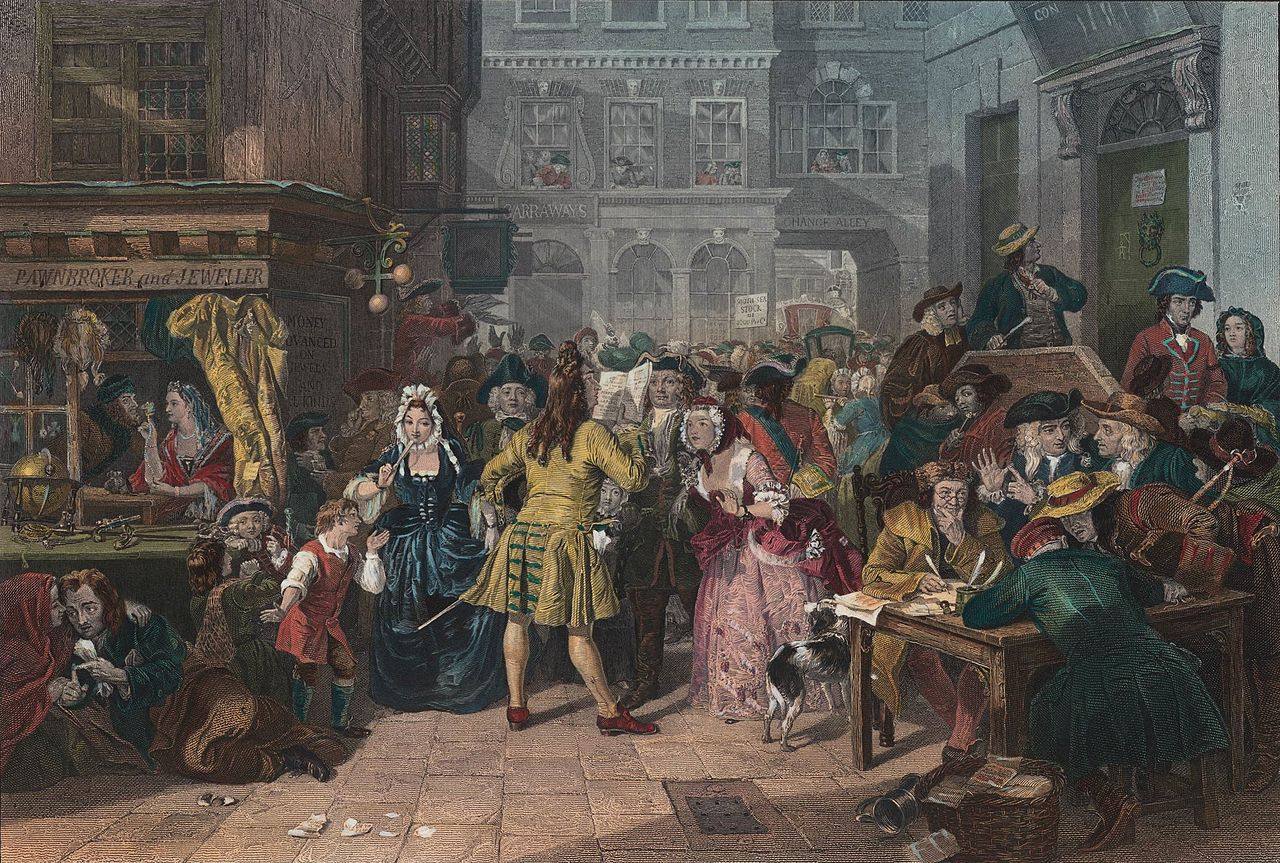
\includegraphics[width=\textwidth]{img/south_sea_bubble.jpg}
\captionsetup{labelformat=empty}
\caption{\small{
Эдвард Мэтью Ворд. \urlnote{Пузырь Компании Южных морей}
{https://commons.wikimedia.org/wiki/File:South_Sea_Bubble.jpg}.
1847 г. Галерея Тейт, Лондон.
}}
\end{figure}
\setcounter{figure}{0}

\clearpage
\tableofcontents

\newcommand{\sectionWithToc}[1] {
	\section*{#1}
	\addcontentsline{toc}{section}{#1}
}

\clearpage
\sectionWithToc{Введение}

В какие ценные бумаги вкладывать деньги? Как накопить на пенсию? Кто такие ETF'ы 
и почему все с ними носятся? Зачем покупать акции, если рынок может упасть? 
Такие вопросы я слышу от студентов и коллег, когда читаю лекции о деривативах. В 
принципе, неудивительно. Деривативы --- это что-то далёкое из мира больших 
банков, а личные инвестиции намного ближе к телу.

Можно было бы ответить коротко <<покупайте индексные фонды, это хорошо!>>. К 
сожалению, такой ответ не объясняет, \emph{почему} это хорошо. Если бы я 
услышал его 15 лет назад, когда ещё не интересовался финансами, то он не нашёл 
бы отклика в моём сердце. Пришлось прослушать не один курс лекций, чтобы 
осознать, какая экономическая теория стоит за этим советом, и начать применять 
его на практике.

Собственно, моя статья это не столько инвестиционный совет (хотя я и расскажу о
личном опыте и даже посчитаю свою <<альфу>>), сколько обзорный курс по теории 
инвестиций. Полезно знать, какие модели придумали предыдущие поколения, и в 
каких терминах можно думать об инвестициях. Если из теории следует, что имеет 
смысл покупать индексные ETF'ы, чтобы копить на пенсию --- так и быть, расскажу 
и об этом.

Не секрет, что в финансах много математики. Я постарался соблюсти баланс. Я 
считаю, что интуитивное понимание главных экономических идей важнее, чем 
конкретная формула. Даже если вы пропустите вообще все формулы, то вы всё равно 
поймёте суть и получите полезные знания. С другой стороны, если вы хотели бы 
размять мозги не ахти какой сложной математикой, то у вас будет такая 
возможность.

\clearpage
\section{Рациональные инвесторы. Риск и доходность. Диверсификация. Портфельная
оптимизация.}

\subsection{Рациональные инвесторы и избегание риска}

Чтобы строить теорию инвестиций, нужно договориться о некоторых свойствах 
инвесторов, которые населяют наш уютный теоретический мирок. Как и большинство 
инвесторов в реальном мире, наши сферические инвесторы будут любить доходность и 
не любить ненужный риск. Из двух инвестиций с одинаковой доходностью они выберут 
ту, что несёт меньший риск. Из двух инвестиций с одинаковым риском они выберут 
ту, что обещает более высокую доходность.

Кому-то может показаться, что \ruen{избегание риска}{risk aversion} --- это
нерациональное поведение слабых духом homo sapiens. На деле же рациональный до
мозга костей homo economicus тоже будет избегать ненужного риска, если мы
сделаем несколько предположений о том, как он принимает решения
\cite[ch.~6.1]{bodie2014investments}.
 
Предположим, что рациональный инвестор максимизирует \ruen{функцию полезности}
{utility function}. Это означает, что все-все-все альтернативы, которые он 
рассматривает, подаются на вход некоторой функции $u(x)$, которая присваивает
каждой альтернативе число --- \ruen{полезность}{utility}. Из множества доступных 
альтернатив рациональный индивид всегда выбирает ту, которая даёт наибольшую
ожидаемую полезность.
 
Допустим, что функция полезности рационального инвестора --- десятичный логарифм
количества долларов на счету. Каждый новый доллар на счету увеличивает
полезность (уровень счастья), потому что логарифм --- возрастающая функция.
Кроме того, каждый следующий доллар приносит меньше счастья, чем
предыдущий, потому что логарифм --- \ruen{выпуклая вверх}{concave}\ функция. 
Никакие другие параметры помимо суммы на счету нашего инвестора не интересуют.
 
Такая форма функции полезности неплохо описывает реальное поведение людей. 
Согласитесь, что пятый подряд шоколадный пончик с шоколадной начинкой и 
шоколадной крошкой приносит меньше удовольствия, чем первый. Точно так же я на 
собственном опыте знаю, что десятый миллиард приносит меньше радости, чем 
первый.
 
Итак, рассмотрим инвестора с логарифмической полезностью. Сейчас у него на счету 
\dollars{100 000}, которые дают полезность $\lg(\num{100 000}) = 5.0$ условных 
единиц счастья.
 
Посмотрите на таблицу \ref{logarithmic_utility_table}. Инвестор должен вложить 
всё своё состояние в один из двух инструментов: либо в абсолютно надёжные 
облигации, либо в рискованные акции. Что бы ни произошло в будущем, облигации 
совершенно точно вырастут на \dollars{5000}, и инвестор через год будет иметь
\dollars{105000}. Акции с вероятностью 50\% вырастут на \dollars{25000} и будут 
стоить \dollars{125000}, либо с вероятностью 50\% упадут на \dollars{15000} и 
будут стоить \dollars{85000}. Математическое ожидание вложения в акции равно 
$0.5 \cdot \dollars{85000} + 0.5 \cdot \dollars{125000} = \dollars{105000}$, то 
есть совпадает с тем, что обещают безрисковые облигации.

\begin{table}[h]
\centering
\begin{tabular}{l|r|r|r|r|r}
\multirow{2}{*}{Сценарий} &
Вероят- &
\multicolumn{2}{c|}{Облигации} &
\multicolumn{2}{c}{Акции} \\
\cline{3-6}
        &  ность   & Капитал    & Полезность & Капитал      & Полезность \\ 
\hline
Хороший & 50\% & \dollars{105000} & 5.021 & \dollars{125000} & 5.097 \\
Плохой  & 50\% & \dollars{105000} & 5.021 & \dollars{85000}  & 4.929 \\ \hline
\multicolumn{2}{l|}{Мат. ожидание} 
& \dollars{105000} & 5.021 & \dollars{105000} & 5.013
\end{tabular}
    \caption{
        Капитал и полезность инвестора в случае инвестиций в облигации или в
        акции.
    }
    \label{logarithmic_utility_table}
\end{table}

Давайте теперь посчитаем полезность. В результате вложения в облигации инвестор 
получит полезность $\lg \num{105000} = 5.021$ условных единиц счастья. Если он 
вложится в акции, то с вероятностью 50\% акции вырастут, и полезность составит
$\lg \dollars{125000} = 5.097$. Однако, с вероятностью 50\% акции упадут, и 
полезность будет равна  $\lg \num{85000} = 4.929$. Средняя ожидаемая полезность 
от инвестиции в акции, таким образом, равна $0.5 \cdot 5.097 + 0.5 \cdot 4.929 = 
5.013$.

Из-за формы функции полезности радость от добавочных \dollars{20 000} 
по сравнению с облигациями в хорошем сценарии ($5.097-5.021 = 0.076$) по модулю 
меньше, чем расстройство от упущенных \dollars{20 000} в плохом сценарии
($4.929 - 5.021 = -0.092$). Потерянные с вероятностью 50\% \dollars{20 000} 
ценнее, чем заработанные с вероятностью 50\% \dollars{20 000}.
  
Так какую же из двух альтернатив выберет наш рациональный инвестор: облигации с 
ожидаемой полезностью 5.021 или акции с ожидаемой полезностью 5.013? Ответ 
очевиден: 5.021 больше, чем 5.013, поэтому инвестор выберет облигации. При 
одинаковой ожидаемой доходности (в обоих случаях ожидаемый капитал составляет
\dollars{105 000}) рациональный инвестор выберет менее рискованную альтернативу, 
то есть проявит то же самое избегание риска, что и реальные биологические 
инвесторы.

Как изменить условие задачи, чтобы инвестор хотя бы воспринимал две альтернативы 
безразлично? Можно, например, пообещать ему более высокую доходность акций в 
хорошем случае. Если акции будут приносить не \dollars{125 000}, а \dollars{129 
706}, то, как показано в таблице \ref{logarithmic_utility_table_premium}, 
ожидаемые полезности двух альтернатив совпадут.

\begin{table}[h]
\centering
\begin{tabular}{l|r|r|r|r|r}
\multirow{2}{*}{Сценарий} & Вероят- & \multicolumn{2}{c|}{Облигации} & 
\multicolumn{2}{c}{Акции} \\
\cline{3-6}
        &  ность   & Капитал    & Полезность & Капитал      & Полезность \\ 
\hline
Хороший & 50\% & \dollars{105000} & 5.021    & \dollars{129706} & 5.113 \\
Плохой  & 50\% & \dollars{105000} & 5.021    & \dollars{85000}  & 4.929 \\ \hline
\multicolumn{2}{l|}{Мат. ожидание}      & \dollars{105000} & 5.021 & \dollars{107353} & 5.021
\end{tabular}
\caption{Капитал и полезность инвестора в случае инвестиций в облигации или в 
акции. Акции имеют более высокую доходность по сравнению с таблицей 
\ref{logarithmic_utility_table}.}
\label{logarithmic_utility_table_premium}
 \end{table}

Чтобы уравнять ожидаемые полезности, нам пришлось улучшить математическое 
ожидание дохода от акций. Раньше акции давали в среднем \dollars{105000}, а 
теперь \dollars{107353}, на \dollars{2353} больше. Эти \dollars{2353} 
дополнительной ожидаемой доходности --- премия за риск (risk premium), которую 
требует инвестор, чтобы рассмотреть возможность покупки акций. Премия за риск 
уравнивает прибавку полезности в хорошем случае ($5.113 - 5.021 = 0.092$) и 
снижение полезности в плохом случае ($5.021 - 4.929 = -0.092$). Если накинуть к 
доходности акций ещё доллар, то инвестор предпочтёт их облигациям.
 
Эти рассуждения верны не только для инвесторов с логарифмической полезностью. 
Достаточно, чтобы функция полезности была возрастающей и выпуклой вверх. Тогда 
инвесторы будут избегать риска и требовать премию (добавочную доходность) от 
рискованных инвестиций. Запомним эту мысль. Она пригодится, когда мы будем 
говорить о теории CAPM.

\subsection{Корреляция с рынком}

Рассмотрим ещё один модельный пример, основанный на идее из лекции профессора
\ruen{Джона Кохрэйна}{John Cochrane} \cite{cochrane2013consumption}.

Есть две акции, A и B, каждая из которых может принести в будущем либо 
\dollars{1000}, либо \dollars{500} с вероятностью 50/50. Акции устроены так, что 
когда акция A приносит \dollars{1000}, акция B приносит \dollars{500}. И 
наоборот, когда A приносит \dollars{500}, B приносит \dollars{1000}. 
Математическое ожидание дохода от каждой акции равно \dollars{750}. При прочих 
равных, какой акцией вы хотели бы владеть? Забудем о цене и предположим, что 
акцию вы получите в подарок.

На первый взгляд, акции совершенно симметричны. Нет никаких рациональных 
аргументов, чтобы предпочесть одну акцию другой. Вы могли бы подбросить монетку, 
положиться на случай и не прогадать. Верно? Не совсем. Что если я уточню, в 
каких именно сценариях акция A приносит \dollars{1000}, а в каких \dollars{500}?

Предположим, что в будущем возможны два сценария. С вероятностью 50\% вы 
потеряете работу или другой источник дохода, и в этом же сценарии акция A будет 
стоить \dollars{1000}, а акция B будет стоить \dollars{500}. С вероятностью 50\% 
вы не только не потеряете работу, а даже получите премию \dollars{10000}, и в 
этом же сценарии акция A будет стоить \dollars{500}, а акция B будет стоить 
\dollars{1000}. Эти альтернативы перечислены в таблице  
\ref{two_shares_states_of_nature}.

\begin{table}[h]
\centering
\begin{tabular}{l|r|r|r}
Сценарий               & Вероятность & Акция A        & Акция B        \\ \hline
Потеря работы          & 50\%        & \dollars{1000} & \dollars{500}  \\
Премия \dollars{10000} & 50\%        & \dollars{500}  & \dollars{1000} \\ \hline
\multicolumn{2}{l|}{Мат. ожидание}   & \dollars{750}  & \dollars{750} 
\end{tabular}
\caption{Две акции дают одинаковый ожидаемый доход, но приносят б\'{о}льшую 
пользу в разных состояниях мира.}
\label{two_shares_states_of_nature}
\end{table}

Когда на лекции я провожу голосование среди студентов (живых людей, а не 
рациональных роботов), все в один голос заявляют, что предпочли бы владеть 
акцией A. Это соответствует простой житейской мудрости. Акция A принесёт 
дополнительные деньги именно в <<плохом>> сценарии, когда каждый доллар на 
счету. Акция A похожа на страховку от потери работы, и поэтому люди её ценят.

Примечательно, что  рациональные логарифмические инвесторы из нашей теории будут 
вести себя точно так же. Поскольку функция полезности выпукла вверх, они будут 
больше ценить акцию A. Акция A приносит больший доход в <<плохом>> сценарии, 
когда каждый дополнительный доллар более ценен. С другой стороны, акция B 
приносит \dollars{1000} в <<хорошем>> сценарии, когда у инвестора и так 
прибавится \dollars{10000}, и добавочная полезность от \dollars{1000} будет не 
столь велика.

Сделаем следующий шаг. Предположим, что в нашей экономике не один рациональный 
инвестор, а множество. Каждый из них предпочтёт ту акцию, которая защитит его от 
потери работы. Что если риск потери работы одним инвестором связан 
(скоррелирован) с потерей работы остальными?  Это вполне разумное предположение. 
Согласитесь, что для большинства людей шансы потерять работу в кризис выше, чем 
в хорошие времена. Кризис потому и кризис, что плохо становится сразу многим 
компаниям, и многие люди теряют работу одновременно.

Получается, что больше инвесторов хотят владеть <<защитной>> акцией A. Если 
инвесторы покупают и продают акции на свободном рынке, то спрос на акцию A будет 
выше, чем спрос на акцию B. При прочих равных, в равновесии акция A будет стоить 
дороже, чем акция B.

Что это означает для доходности инвестиций в акцию A и акцию B? Для начала 
давайте договоримся о формальном определении, что такое доходность. Допустим, 
что вы купили актив (акцию, облигацию, квартиру) в момент времени $t$ по цене 
$P_t$, а в момент времени $t+1$ актив стал стоить $P_{t+1}$. Кроме того, вы 
получили от актива денежную выплату (дивиденды, купон, арендную плату)
$D_{t+1}$. Тогда ваша полная доходность за период времени между $t$ и $t+1$ 
составила
\begin{equation}
R_{t+1} = \dfrac{P_{t+1} + D_{t+1}}{P_t} - 1
\label{total_return_formula}
\end{equation}

Например, предположим, что инвестор купил акцию B за $P_t = \dollars{600}$. 
Реализовался <<хороший>> сценарий, и акция стала стоить $P_{t+1} = 
\dollars{1000}$ и не заплатила никаких дивидендов ($D_{t+1} = \dollars{0}$). 
Тогда инвестор заработал $\dollars{1000}/\dollars{600} - 1 \approx 66.7\%$.

Если считать, что будущая цена $P_{t+1}$ и будущие дивиденды $D_{t+1}$ это 
случайные величины, то будущая доходность $R_{t+1}$ это тоже случайная величина. 
Поэтому формулу (\ref{total_return_formula}) можно записать и для математических 
ожиданий.
\begin{equation}
\mathbb{E}(R_{t+1}) = \dfrac{\mathbb{E}(P_{t+1}) + \mathbb{E}(D_{t+1})}{P_t} - 1
\label{total_return_formula_exp}
\end{equation}

Выглядит как урок арифметики для старшей группы детского садика, но он 
показывает нам важную деталь. Текущая цена $P_t$ стоит в формулах 
(\ref{total_return_formula}) и (\ref{total_return_formula_exp}) в знаменателе, 
поэтому при той же будущей цене и будущих дивидендах более низкая цена сегодня 
означает б\'{о}льшую ожидаемую доходность в будущем.

Как мы выяснили, инвесторы будут предпочитать акцию A акции B. Если инвесторы не 
получают акции в подарок, а покупают их на рынке, то спрос на акцию A окажется 
выше, чем на акцию B. Следовательно, в равновесии цена акции B должна быть ниже, 
а ожидаемая доходность выше! Например, если рынок оценит акцию A в 
\dollars{700}, а акцию B в \dollars{650}, то по формуле
(\ref{total_return_formula_exp}) ожидаемая доходность акции A составит 
$\dollars{750}/\dollars{700} - 1 \approx 7.1\%$, а акции B --- 
$\dollars{750}/\dollars{650} - 1 \approx 15.3\%$.

Таким образом, инвесторы будут зарабатывать более высокую доходность
(б\'{о}льшую премию за риск) на активах, похожих на акцию B. Это те активы, 
которые сильнее связаны с общим состоянием экономики, то есть растут в хорошие 
времена и падают в плохие. Поставим крестик, чтобы вернуться к этой идее позже, 
когда будем изучать CAPM.

\subsection{Вспоминаем теорию вероятностей}

Чтобы продолжать строить теорию, нам нужно воспользоваться несколькими 
тривиальными фактами из теории вероятностей. Вы можете смело пропустить этот 
раздел, если вам не составляет труда прочитать и понять следующую фразу: 
<<дисперсия суммы --- это сумма дисперсий плюс две ковариации>>.

Я предполагаю, что все более-менее интуитивное понимают, что такое 
математическое ожидание случайной величины. Для наших целей совершенно нет 
необходимости знать, что это интеграл Лебега. Достаточно простой интуиции, что 
мат. ожидание --- это среднее значение случайной величины. Я буду обозначать 
мат. ожидание случайной величины $X$ как $\mathbb{E}(X)$.

Например, если мы бросаем игральный кубик, то выпавшее количество очков --- это 
случайная величина $X$, которая имеет мат. ожидание
\begin{align*}
\mathbb{E}(X) = \dfrac{1}{6}\cdot 1 + \dfrac{1}{6}\cdot 2
+ ... + \dfrac{1}{6}\cdot 6 = 3.5
\end{align*}

Важное свойство мат. ожидания --- линейность. Например, если я бросаю не один 
кубик, а четыре, и складываю выпавшие очки, то мат. ожидание суммы будет равно 
$4 \cdot 3.5 =  14$. Формально это можно записать так ($\alpha$ и $\beta$ --- 
константы, $X$ и $Y$ --- случайные величины):
\begin{equation*}
\mathbb{E}(\alpha X + \beta Y) = \alpha\mathbb{E}(X) + \beta\mathbb{E}(Y)
\end{equation*}

Дисперсия случайной величины показывает, насколько велик разброс значений вокруг 
среднего. Чем больше разброс (например, чем дальше друг от друга минимум и 
максимум), тем больше дисперсия. Стандартное отклонение --- это квадратный 
корень из дисперсии. Я буду обозначать дисперсию случайной величины $X$ как  
$Var(X)$, а её стандартное отклонение как $\sigma_X$.
\begin{equation*}
Var(X) = \sigma_X^2 = \mathbb{E}\left[(X - \mathbb{E}(X))^2 \right]
\end{equation*}

В примере с игральным кубиком дисперсия будет равна
\begin{equation*}
Var(X) = \dfrac{(1 - 3.5)^2 + (2 - 3.5)^2 + ... + (6 - 3.5)^2}{6} \approx 2.92
\end{equation*}

Предположим, что у нас есть две случайные величины $X$ и $Y$. Резонно задать 
вопрос: а есть ли связь между $X$ и $Y$? Например, верно ли, что б\'{о}льшие 
значения $X$ чаще выпадают одновременно с б\'{о}льшими значениями $Y$? Ответ на 
этот вопрос дают ковариация, которую я буду обозначать $Cov(X,Y)$, и коэффициент 
корреляции, который я обозначу $\rho_{X,Y}$.
\begin{equation*}
Cov(X,Y) = \rho_{X,Y}\sigma_X\sigma_Y 
= \mathbb{E}\left[(X - \mathbb{E}(X))(Y - \mathbb{E}(Y)) \right]
\end{equation*}

Чтобы визуализировать идею корреляции, я четыре раза попросил компьютер 
сгенерировать по 250 случайных реализаций стандартных нормальных величин $X$ и 
$Y$. Четыре эксперимента отличаются только корреляциями между $X$ и $Y$. 
Результаты представлены на рисунке \ref{covariance_example}. Как видите, чем 
ближе корреляция к 1, тем очевиднее линейная связь между $X$ и $Y$.

\begin{figure}[h]
\centering
\begin{tikzpicture}
\begin{groupplot}[
    width = \textwidth / 3.5,
    height = \textwidth / 3.5,
    group style = {group size = 4 by 1},
    xmin = -4, xmax=4,
    ymin = -4, ymax=4
]

    \newcommand{\addCovarianceSubplot}[3]{
        \nextgroupplot[
            title = {$\rho_{X,Y} = #1$}
        ]
        \addplot[
            color = Set1-B,
            only marks
        ]
        table[
            x = #2,
            y = #3,
            col sep=comma
        ]
        {data/covariance_plot_random_samples.csv};
    }
    
    \addCovarianceSubplot{0.0}{X0}{Y0}
    
    \addCovarianceSubplot{0.25}{X25}{Y25}
    
    \addCovarianceSubplot{0.75}{X75}{Y75}
    
    \addCovarianceSubplot{1.0}{X100}{Y100}
    
\end{groupplot}
\end{tikzpicture}
\caption{Реализации случайных величин $X$ и $Y$ в зависимости от корреляции 
между ними.}
\label{covariance_example}
\end{figure}

Нам понадобится правило для вычисления дисперсии суммы случайных величин. 
Дисперсия суммы зависит как от дисперсии слагаемых, так и от ковариации (или от 
корреляции) между ними:
\begin{align}
Var(\alpha X + \beta Y)
&=
\alpha^2 Var(X) + \beta^2 Var(Y) + 2 \alpha \beta Cov(X, Y) = \nonumber \\
&=
\alpha^2\sigma_X^2 + \beta^2 \sigma_Y^2 
+ 2\alpha\beta\rho_{X,Y}\sigma_X\sigma_Y
\label{variance_of_linear_combination}
\end{align}

\subsection{Диверисификация, или о пользе корреляций}

Если бы я мог дать вам всего один совет касательно инвестиций, то я бы сказал 
<<диверсифицируйтесь!>>. Или, следуя народной мудрости, не кладите все яйца в 
одну корзину. 

Есть несколько довольно популярных заблуждений по поводу диверсификации. Первое 
--- что диверсификация уменьшает доходность. Второе --- что диверсификация 
возможна, только если активы, в которые вы инвестируете, связаны отрицательной 
корреляцией. Это не так, и если вы, как и остальные инвесторы, не любите риск и 
любите доходность, то вы можете улучшить баланс риска и доходности с помощью 
диверсификации.

Рассмотрим пример. Пусть у нас есть всего две акции, $X$ и $Y$. Мы знаем, что 
они имеют одинаковую ожидаемую доходность $\mu=5\%$ и одинаковое стандартное 
отклонение $\sigma=10\%$. Кроме того, они связаны друг с другом корреляцией
$\rho_{X,Y} = 0.4$. Вы должны вложить долю $w$ своего капитала в акции $X$, а 
долю $(1-w)$ --- в акции $Y$.

Зависит ли ожидаемая доходность ваших инвестиций от выбора $w$? Нет, не зависит. 
Из линейности мат. ожидания следует, что при любом выборе $w$ вы всегда получите 
одну и ту же ожидаемую доходность 5\%:
\begin{equation*}
\mathbb{E}\left[ wX + (1-w)Y\right] =
w\mathbb{E}(X) + (1-w)\mathbb{E}(Y) = w\mu + (1-w)\mu = \mu = 5\%
\end{equation*}

А что с риском? Из формулы (\ref{variance_of_linear_combination}) следует, что 
дисперсия и стандартное отклонение зависят не только от стандартного отклонения 
каждой акции, но и от корреляции между ними:
\begin{align*}
Var(wX + (1-w)Y)
&= w^2Var(X) + (1-w)^2Var(Y) + 2w(1-w)Cov(X,Y) = \\
&= w^2\sigma^2 + (1-w)^2\sigma^2 + 2w(1-w)\rho_{X,Y}\sigma^2 = \\
&= \sigma^2\left(w^2 + (1-w)^2 + 2w(1-w)\rho_{X,Y} \right)
\end{align*}

Невооружённым глазом видно, что дисперсия портфеля (то есть риск) есть 
квадратичная функция от $w$. Стало быть, при каком-то $w$ она должна достигать 
минимума. Как показано на рисунке \ref{portfolio_volatility_vs_w}, этот минимум 
действительно достигается при $w=0.5$, то есть если вы инвестируете половину 
капитала в акции $X$ и половину в акции $Y$. Стандартное отклонение доходности 
вашего портфеля составит 8.37\%. С другой стороны, если бы вы инвестировали все 
деньги только в акцию $X$ (или наоборот, только в акцию $Y$), то вам бы пришлось 
смириться со стандартным отклонением целых 10\%.

\begin{figure}[h]
\centering
\begin{tikzpicture}
\begin{axis}[
    width = \textwidth * 0.5,
    xlabel = {$w$ --- доля инвестиций в акцию $X$},
    ylabel = {Ст. откл. портфеля, \%},
    xmin = 0,
    xmax = 1,
    ymin = 0,
    ymax = 10,
    yticklabel = {$\pgfmathprintnumber{\tick}$}
]
    \addplot[
        color = Set1-B,
        line width = 1pt,
        samples at = {0,0.05,...,1}
	 ]
    {10 * sqrt(x^2 + (1-x)^2 + 2*0.4*x*(1-x))};

	 \draw[
        color=black,
        dashed
    ]
    (axis cs: 0.5, 0) -- (axis cs: 0.5, 8.366) -- (axis cs: 0, 8.366);

    \node[
        anchor=north west
    ]
    at (axis cs: 0.5, 8.366)
    {(0.5, 8.37\%)};

    \node[
        color=Set1-B,
        circle,
        fill, 
        inner sep=2pt
    ]
    at (axis cs: 0.5, 8.366) {};
\end{axis}
\end{tikzpicture}
\caption{Зависимость стандартного отклонения доходности портфеля от доли 
инвестиций в акцию $X$.}
\label{portfolio_volatility_vs_w}
\end{figure}

Вывод: вам не нужно искать активы с отрицательной корреляцией, чтобы 
воспользоваться плодами диверсификации! Вполне достаточно, чтобы корреляция была 
отлична от 1.0. Диверсификация может снизить риск ваших инвестиций при той же 
ожидаемой доходности или дать б\'{о}льшую доходность при неизменном уровне 
риска.

\subsection{Портфельная оптимизация}

Давайте обобщим наш замечательный пример с двумя акциями на случай, когда мы 
составляем портфель из произвольного числа активов. При этом каждый актив 
обладает собственной ожидаемой доходностью и дисперсией.

Допустим, что нам известны ожидаемые доходности четырёх классов активов: акций, 
облигаций, \ruen{инвестиционных фондов недвижимости}{real estate investment 
trust, REIT} и золота. Также мы знаем стандартные отклонения и корреляции между 
активами. Эти значения приведены в таблице \ref{asset_class_returns_table}.

\begin{table}[h]
\centering
\begin{tabular}{l|r|r|r|r|r|r}
 & \multicolumn{2}{c|}{Доходность} & \multicolumn{4}{c}{Корреляция} \\ 
\cline{2-7}
Актив        & Среднее & Ст. откл. & Акц. & Обл. & Нед. & Зол. \\ \hline
Акции        & 10.9\%  & 15.2\%    & 1.00  & 0.00   & 0.59    & 0.04 \\
Облигации    & 5.2\%   & 3.6\%     & 0.00  & 1.00   & 0.19    & 0.28 \\
Недвижимость & 10.8\%  & 19.2\%    & 0.59  & 0.19   & 1.00    & 0.13 \\
Золото       & 7.0\%   & 15.6\%    & 0.04  & 0.28   & 0.13    & 1.00
\end{tabular}
\caption{Средние доходности, стандартные отклонения и корреляции между классами 
активов. Период 1994--2020 по данным сайта \urlnote{Portfolio Visualizer}
{https://www.portfoliovisualizer.com/efficient-frontier}.}
\label{asset_class_returns_table}
\end{table}

Как видите, я использовал \emph{исторические} данные, чтобы оценить параметры 
распределения \emph{будущих} доходностей активов. Это довольно опасное занятие, 
потому что прошлое не предсказывает будущее. В идеале, я должен был бы нанять 
аналитика, который выдал бы мне ожидаемые будущие доходности исходя из научного 
прогноза, а не исходя из средней доходности в прошлом. К сожалению, редкий 
прогноз на финансовых рынках оказывается точнее, чем <<будет как раньше>>. 
Впрочем, для нашей цели проиллюстрировать принцип диверсификации это не так 
важно.

Итак, вы --- инвестор, который любит доходность и не любит дисперсию. Вам нужно 
распределить свой капитал между четырьмя активами. Какую пропорцию между 
акциями, облигациями, недвижимостью и золотом выбрать?

Разумно задать следующий вопрос: если вы хотите получить ожидаемую доходность, 
скажем 10\%, то какой портфель (какая пропорция акций, облигаций, недвижимости и 
золота) обеспечат такую доходность? А если таких возможных портфелей несколько 
(что вполне возможно), то который из них будет наименее рискованным (дисперсия и 
стандартное отклонение будут меньше, чем у остальных портфелей с такой 
доходностью)?

Рисунок \ref{efficient_frontier} отвечает на этот вопрос. Каждая точка на 
графике --- это гипотетический портфель, который характеризуется стандартным 
отклонением (ось $x$) и ожидаемой доходностью (ось $y$). Для каждого уровня 
желаемой доходности я рассчитал (как --- расскажу позже) оптимальный портфель, 
то есть портфель с наименьшим стандартным отклонением из всех портфелей с данной 
доходностью.

\begin{figure}[h]
\centering
\begin{tikzpicture}
\begin{axis}[
    width = \textwidth,
    xlabel = {Стандартное отклонение, \%},
    ylabel = {Ожидаемая доходность, \%},
    xmin = 0, xmax = 21,
    ymin = 0, ymax = 13
]

    \newcommand{\drawAssetNode}[3]{
        \node[
            circle,
            fill,
            inner sep=2pt
        ] at (axis cs: #1, #2) {};
        \node[
            anchor=north
        ]
        at (axis cs: #1, #2)
        {\small #3};
    }

    \newcommand{\drawPortfolioNode}[8]{
        \node[
            anchor=#8
        ] at (axis cs: #1, #2) {
	         \small
	         \begin{tabular}{|l|r|}
		      \hline
		      \multicolumn{2}{|c|}{#3} \\ \hline
		      Акц. & #4\% \\
		      Обл. & #5\% \\
		      Нед. & #6\%  \\
		      Зол. & #7\% \\
		      \hline
		      \end{tabular}
        };
	 
	     \node[
	         circle,
	         fill,
	         inner sep=3pt,
	         color=Set1-B
        ] at (axis cs:#1, #2) {};
    }

    \addplot[
        line width=1pt,
        color=Set1-B
    ]
    table[
        x=std_dev,
        y=target_return,
        col sep=comma
    ]
    {data/efficient_frontier_plot_data.csv};

    \drawAssetNode{15.2}{10.9}{Акции}

    \drawAssetNode{3.6}{5.2}{Облигации}

    \drawAssetNode{19.2}{10.8}{Недвиж.}

    \drawAssetNode{15.6}{7.0}{Золото}

    \drawPortfolioNode{4.40}{6.5}{Портфель A}{21.2}{74.6}{0.5}{3.7}{south east}

    \drawPortfolioNode{12.0}{9.95}{Портфель B}{63.2}{3.5}{14.4}{18.9}{south east}

    \drawPortfolioNode{12.0}{6.5}{Портфель C}{0.0}{30.0}{0.0}{70.0}{north east}

    \draw[dashed] (axis cs: 12.0, 9.95) -- (axis cs: 12.0, 0);
    \draw[dashed] (axis cs: 0.0, 6.5) -- (axis cs: 12.0, 6.5);
    \draw[dashed] (axis cs: 0, 9.95) -- (axis cs: 12.0, 9.95);
    \draw[dashed] (axis cs: 4.40, 0) -- (axis cs: 4.40, 6.5);

\end{axis}
\end{tikzpicture}

\caption{Граница эффективности для портфелей, составленных из акций, облигаций, 
недвижимости и золота.}
\label{efficient_frontier}
\end{figure}

Синяя линия на графике --- это так называемая \ruen{граница эффективности}
{efficient frontier}. Именно на ней лежат оптимальные портфели, имеющие 
минимальное стандартное отклонение при заданной доходности. Рациональный 
инвестор будет стремиться выбрать один из портфелей на этой линии, потому что 
любой другой портфель будет заведомо хуже.

Например, совершенно нет смысла выбирать портфель C, состоящий на 30\% из 
облигаций и на 70\% из золота. Этот портфель имеет ожидаемую доходность 6.5\% 
при стандартном отклонении 12\%. Однако, раз уж вы согласны принять на себя риск 
в 12\%, то за этот риск вы можете получить более высокую доходность --- почти 
10\% в портфеле B (63.2\% в акциях). С другой стороны, если вы готовы 
удовлетвориться ожидаемой доходностью 6.5\%, то лучше выбрать менее рискованный 
портфель A (74.6\% в облигациях), который имеет стандартное отклонение 4.4\%.

Другими словами, вы всегда стремитесь выбрать портфель, который лежит выше 
(больше доходность) и левее (меньше риск). В какой-то момент вы упрётесь в 
границу эффективности и не сможете двигаться дальше --- не получится заработать 
15\% при стандартном отклонении 2\%. Очутившись на границе эффективности, вы 
можете гулять по ней либо вправо-вверх (больше риск, больше доходность), либо 
влево-вниз (ниже риск, ниже доходность). То, на каком из оптимальных портфелей 
на границе эффективности остановитесь именно вы, зависит от вашей личной 
чувствительности к риску.

Обратите внимание, что граница эффективности лежит выше или левее, чем отдельные 
активы --- облигации, золото, недвижимость. Мы снова возвращаемся к идее 
диверсификации. Если вы держите все инвестиции в одном активе, то скорее всего 
вы могли бы получать такую же доходность при меньшем уровне риска, если бы 
диверсифицировались. Чаще всего на границе эффективности оказываются портфели, 
составленные из нескольких активов.

Рисунок \ref{efficient_frontier_allocation} показывает, как изменяется состав 
оптимального портфеля по мере того как вы движетесь по границе эффективности 
слева направо (от меньшего риска к большему риску). Вполне ожидаемо, наименее 
рискованные портфели состоят в основном из облигаций, а наиболее рискованные --- 
из акций и недвижимости.

\begin{figure}[h]
\centering
\begin{tikzpicture}
\begin{axis}[
    width = \textwidth,
    height = \textwidth/2,
    xlabel = {Стандартное отклонение, \%},
    ylabel = {Доля актива, \%},
    xmin = 3.5,
    xmax = 15.2,
    ymin = 0,
    ymax = 100,
    stack plots = y
]

    \newcommand{\addAssetAreaChart}[2] {
        \addplot[
            fill = #2
        ]
        table[
            x = std_dev,
            y = #1,
            col sep = comma
        ]
        {data/efficient_frontier_plot_data.csv}
        \closedcycle;
    }

    \newcommand{\addAssetLabel}[2] {
        \node
        at (axis cs: 9.3, #2)
        {\small #1};
    }
    
    \addAssetLabel{Акции}{25}
    \addAssetLabel{Облигации}{63}
    \addAssetLabel{Недвиж.}{82}
    \addAssetLabel{Золото}{93}
    
    \addAssetAreaChart{stocks}{Pastel2-C}
    \addAssetAreaChart{bonds}{Pastel2-D}
    \addAssetAreaChart{reit}{Pastel2-E}
    \addAssetAreaChart{gold}{Pastel2-F}
\end{axis}
\end{tikzpicture}

\caption{Состав портфелей на границе эффективности.}
\label{efficient_frontier_allocation}
\end{figure}

В подтверждение тезиса о диверсификации, единственный оптимальный портфель, 
который состоит только из одного актива (акций) --- это портфель с максимальной 
доходностью и максимальным риском. Это ожидаемо, потому что в условии задачи 
именно акции имеют максимальную доходность 10.9\%. Если хоть немного разбавить 
акции другим активом с меньшей доходностью, то общая доходность портфеля упадёт. 
Так что инвестор, который желает выжать максимально возможную доходность, будет 
вынужден составить портфель только из акций.

\subsection{Квадратичное программирование}

В предыдущем разделе я обещал рассказать, как именно я посчитал оптимальные 
портфели. В этом разделе я выполню обещание и объясню, как формально поставить 
задачу выбора оптимального портфеля на языке математики. Если вам не очень 
интересны математические подробности, то вы можете смело перейти к следующему 
разделу. Незнание этих выкладок не помешает вам продолжить читать статью и 
извлечь из неё пользу.

Если вы всё ещё со мной, то, как говорил известный сатирик, наберите воздуха в 
грудь.

Итак, у нас есть $n$ активов. Будущая доходность $i$-го актива --- это случайная 
величина со средним $\mu_i$ и стандартным отклонением $\sigma_i$. Доходности 
$i$-го и $j$-го актива связаны корреляцией $\rho_{i,j}$.

Нас просят распределить единичный капитал между активами. Более формально,
$i$-му активу нужно присвоить вес (долю в портфеле) $x_i$. Потребуем, чтобы все 
веса $x_i$ были положительными (нельзя продать актив, которого у нас нет), а их 
сумма равнялась единице (мы должны распределить весь капитал без остатка). 

Для начала введём несколько удобных матричных обозначений, то есть запишем 
параметры задачи в аккуратные прямоугольные таблицы.
\begin{align*}
x = \begin{bmatrix}x_1 \\ x_2 \\ \vdots \\ x_n\end{bmatrix}
\qquad
\mu = \begin{bmatrix}\mu_1 \\ \mu_2 \\ \vdots \\ \mu_n\end{bmatrix}
\qquad
S = \begin{bmatrix}
\sigma_1^2 & \rho_{1,2}\sigma_1\sigma_2 & \cdots & \rho_{1,n}\sigma_1\sigma_n \\
\rho_{2,1}\sigma_2\sigma_1 & \sigma_2^2 & \cdots & \rho_{2,n}\sigma_2\sigma_n \\
\vdots & \vdots & \ddots & \vdots \\
\rho_{n,1}\sigma_n\sigma_1 & \rho_{n,2}\sigma_n\sigma_2 & \cdots & \sigma_n^2
\end{bmatrix}
\qquad
e = \begin{bmatrix}1 \\ 1 \\ \vdots \\ 1\end{bmatrix}
\end{align*}

Утверждается, что вопрос <<какой портфель с ожидаемой доходностью $r$ имеет 
наименьшую дисперсию?>> можно формально записать в виде следующей задачи 
минимизации:
\begin{align}
\begin{cases}
x^TSx \to \min \\
\mu^Tx = r \\
e^Tx = 1 \\
x \ge 0
\end{cases}
\label{portfolio_optimization_statement}
\end{align}

Вид формул (\ref{portfolio_optimization_statement}) вызывает у разных людей 
противоположные эмоции. Например, человек, знакомый с теорией математической 
оптимизации, воскликнет: <<Батюшки, да это же банальный QP! Стоило ли ради этого 
писать столько текста?>>.

Действительно, хорошая новость заключается в том, что человечество уже давно 
научилось решать задачи такого вида и даже дало им специальное название --- 
\ruen{квадратичное программирование}{quadratic programming, QP} \cite[ch.~7--8]
{cornuejols2006optimization}. Почти для любого языка программирования, от C до 
Питона, найдётся готовая библиотека для решения этой задачи. Достаточно ничего 
не напутать и правильно составить матрицы $\mu$, $S$ и $e$, а дальше библиотека 
сама найдёт оптимальное решение. Совершенно не обязательно разбираться в том, 
какой алгоритм поиска решения крутится под капотом.

С другой стороны, у неподготовленного человека такая постановка задачи может 
вызвать ступор. Давайте пройдёмся по ней строчка за строчкой, чтобы убедиться, 
что в ней нет никакой тёмной магии.

Что такое $x^TSx$? Это компактная запись дисперсии портфеля, составленного с 
весами $x_i$. Для наглядности можно расписать это выражение для случая двух 
активов ($n=2$) и перемножить матрицы как нас учили на первом курсе, строка на 
столбец. Получится уже знакомая нам формула 
(\ref{variance_of_linear_combination}), связывающая дисперсию суммы с 
ковариацией:
\begin{align*}
x^TSx &= 
\begin{bmatrix}x_1 & x_2\end{bmatrix}
\begin{bmatrix}
\sigma_1^2 & \rho_{1,2}\sigma_1\sigma_2 \\
\rho_{1,2}\sigma_1\sigma_2 & \sigma_2^2
\end{bmatrix}
\begin{bmatrix}
x_1 \\
x_2
\end{bmatrix}
=
\begin{bmatrix}x_1 & x_2\end{bmatrix}
\begin{bmatrix}
x_1\sigma_1^2 + x_2\rho_{1,2}\sigma_1\sigma_2 \\
x_1\rho_{1,2}\sigma_1\sigma_2 + x_2\sigma_2^2
\end{bmatrix} = \\
&= 
x_1^2\sigma_1^2 + 2x_1x_2\rho_{1,2}\sigma_1\sigma_2 + x_2^2\sigma_2^2
\end{align*}

Следовательно, если мы попросим алгоритм минимизировать значение $x^TSx$, то он 
постарается найти портфель (набор весов $x_i$) с минимальной дисперсией.

Если не дать алгоритму оптимизации никаких ограничений, то он довольно быстро 
скажет вам, что портфель с минимальной дисперсией --- это портфель с нулевыми 
весами. Действительно, если ничего не инвестировать, то и риска никакого не 
будет. Однако, это не совсем то, что мы хотим, поэтому нам нужно добавить в 
задачу дополнительные \ruen{ограничения}{constraints}.

Первое условие --- это $\mu^Tx = r$. По-русски, мы просим алгоритм рассматривать 
только те портфели, которые имеют ожидаемую доходность $r$. В самом деле, если 
расписать матричное умножение, то получится сумма $\mu_1x_1 + ... + \mu_nx_n$, 
то есть ожидаемая доходность портфеля.

Второе условие --- это $e^Tx = 1$. Его можно записать как $x_1 + ... + x_n = 1$. 
Мы говорим алгоритму, что корректное решение (набор весов $x_i$) --- это когда 
весь единичный капитал распределён между активами и ни один рубль не остался 
неинвестированным.

Наконец, третье условие $x \ge 0$ просто говорит, что все веса $x_i$ должны быть 
неотрицательными (можно только покупать активы в портфель, но нельзя продавать).

Всё, заканчиваю стращать вас математикой. В сухом остатке, мы всегда можем найти 
оптимальный портфель, то есть портфель с минимальной дисперсией, для заданной 
ожидаемой доходности $r$. Для этого нужно составить несколько матриц и скормить 
их алгоритму квадратичного программирования.

\clearpage
\section{Модель CAPM. Систематический риск. Рыночная премия за риск.}

\begin{figure}[h]
\centering
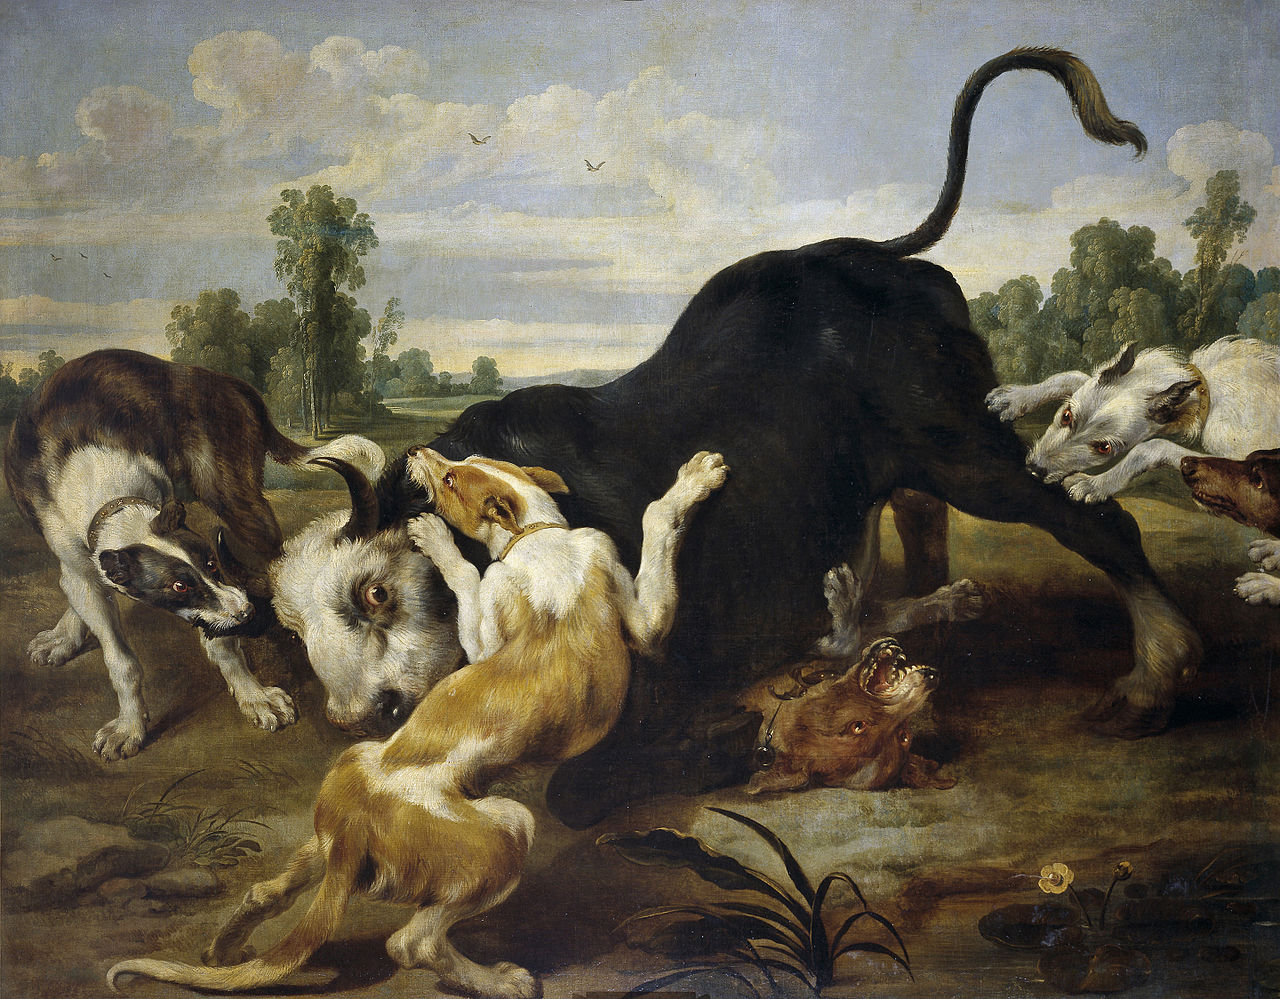
\includegraphics[width=\textwidth]{img/bull_subdued_by_dogs.jpg}
\captionsetup{labelformat=empty}
\caption{\small{
Пауль де Вос. \urlnote{Бык, поверженный собаками}
{https://commons.wikimedia.org/wiki/File:Paul_de_Vos_-_Bull_subdued_by_dogs.jpg}.
1638--1640 гг. Музей Прадо, Мадрид.
}}
\end{figure}
\setcounter{figure}{0}

\subsection{Оптимизация с безрисковым активом}

Продолжим изучать задачу оптимизации портфеля. Неужели теперь каждый инвестор 
должен учить эту теорию и умножать в уме матрицы на 500 строк, чтобы собрать 
оптимальный портфель? К счастью, если добавить в задачу ещё кое-что, то 
математика резко упрощается.

Предположим, что на рынке есть не только четыре актива из таблицы 
\ref{asset_class_returns_table}, но и особый \ruen{безрисковый}{risk free} 
актив, который имеет нулевое стандартное отклонение. Проще говоря, будущая 
доходность безрискового актива --- это не случайная величина, а константа. 

Примером такого актива могут быть краткосрочные облигации Казначейства США 
(Treasury bills). Если вы сейчас покупаете за \dollars{999} облигацию, по 
которой через месяц правительство США обязуется выплатить \dollars{1000}, то вы 
точно знаете свою будущую доходность. По формуле (\ref{total_return_formula}) 
получается $\dollars{1000}/\dollars{999} - 1 \approx 0.1\%$. Не так много, зато 
наверняка. За последние 230 лет был всего один случай, когда из-за 
нерасторопности бухгалтерии выплаты задержались на несколько дней 
\cite{marron2011default}, но ничего серьёзнее пока не случалось.

Итак, добавим к нашим четырём активам пятый --- безрисковые облигации с 
ожидаемой доходностью 4\% (чтобы график выглядел симпатично) и стандартным 
отклонением 0\%. Кроме того, сделаем ещё одно допущение. Предположим, что 
инвесторы в нашей могут занимать деньги под безрисковую процентную ставку (то 
есть под 4\%). Тогда новая граница эффективности будет выглядеть как на рисунке 
\ref{efficient_frontier_with_risk_free}.

\begin{figure}[h]
\centering
\begin{tikzpicture}
\begin{axis}[
    width=\textwidth,
    xlabel={Стандартное отклонение, \%},
    ylabel={Ожидаемая доходность, \%},
    xmin=0, xmax=14,
    ymin=0, ymax=10
]

\newcommand{\drawAssetNode}[4]{
    \node[circle,fill,inner sep=2pt] at (axis cs: #1, #2) {};
    \node[anchor=#4] at (axis cs: #1, #2) {\small #3};
}

\newcommand{\drawPortfolioNode}[8]{\node[anchor=#8] at (axis cs: #1, #2) {
		\small \begin{tabular}{|l|r|}
		\hline
		\multicolumn{2}{|c|}{#3} \\ \hline
		Акц. & #4\% \\
		Обл. & #5\% \\
		Нед. & #6\%  \\
		Зол. & #7\% \\
		\hline
		\end{tabular}
	};
	\node[circle, fill, inner sep=3pt, color=Set1-B] at (axis cs:#1, #2) {};
}

\newcommand{\drawPortfolioNodeTwo}[6]{
\node[anchor=#6] at (axis cs: #1, #2) {
		\small \begin{tabular}{|l|r|}
		\hline
		\multicolumn{2}{|c|}{#3} \\ \hline
		Портф. T & #4\% \\
		Безриск. & #5\% \\
		\hline
		\end{tabular}
	};
	\node[circle, fill, inner sep=3pt, color=Set1-B] at (axis cs:#1, #2) {};
}

\addplot[line width=1pt, color=Set1-B, domain=0:21] {4 + x * (6.75 - 4) / 4.83};

\drawPortfolioNodeTwo{1.45}{4.83}{Портфель А}{30}{70}{north west}

\drawPortfolioNodeTwo{4.83}{6.75}{Портфель B}{100}{0}{north west}

\drawPortfolioNodeTwo{7.25}{8.12}{Портфель C}{150}{-50}{north west}

\drawAssetNode{0.0}{4.0}{}{west}

\drawPortfolioNode{4.83}{6.75}{Портфель T}{24.2}{69.5}{1.5}{4.8}{south east}

\addplot[
    line width=1pt,
    color=Set1-B,
    dashed
]
table[
    x=std_dev, 
    y=target_return, 
    col sep=comma
]
{data/efficient_frontier_plot_data.csv};

\end{axis}
\end{tikzpicture}

\caption{Граница эффективности для портфелей, составленных из акций, облигаций, 
недвижимости, золота и безрискового актива.}
\label{efficient_frontier_with_risk_free}
\end{figure}

Сплошная синяя линия --- это новая граница эффективности для портфелей из 
четырёх рискованных активов и безрискового актива. Пунктирная линия --- это 
старая граница эффективности с рисунка \ref{efficient_frontier} для портфелей из 
четырёх рискованных активов. Можно строго математически доказать несколько 
фактов об этих двух линиях.

Во-первых, новая и старая граница касаются ровно в одной точке. Портфель T, 
который соответствует этой точке, так и называется --- касательным (tangent). 
Этот портфель состоит из всех рискованных активов, которые у нас были раньше, но 
не содержит безрисковый актив.

Во-вторых, граница эффективности с безрисковым активом --- это прямая линия. 
Любой портфель на этой границе можно представить как комбинацию безрискового 
актива и касательного портфеля.

Например, инвестор может вложить 70\% своего капитала в безрисковый актив, а 
30\% --- в касательный портфель (то есть распределить 30\% между четырьмя 
рискованными активами пропорционально их весам в касательном портфеле). Тогда у 
него получится портфель A, который лежит на границе эффективности и имеет 
стандартное отклонение 1.5\% при ожидаемой доходности 4.8\%.

Ранее мы щедро предоставили инвестору опцию занять деньги под безрисковую 
процентную ставку. Предположим, что инвестор займёт сумму, равную половине 
своего начального капитала, а затем вложит всё (и свои деньги, и заёмные) в 
касательный портфель. Тогда он окажется в точке C, которая лежит выше старой 
границы эффективности и была бы для него недоступна, если бы он не мог занимать 
деньги.

Выбирая пропорцию между безрисковым активом и касательным портфелем рискованных 
активов, инвесторы могут гулять по прямой границе эффективности вверх и вниз. 
Увеличиваем долю безрискового актива --- спускаемся влево в зону меньшей 
доходности и меньшего риска. Уменьшаем долю безрискового актива (или даже 
занимаем деньги) --- поднимаемся вправо к более высокому риску и ожидаемой 
доходности. 

На рынке может быть множество инвесторов, каждый со своей индивидуальной 
чувствительностью к риску. Каждый выберет комфортное лично ему сочетание риска и 
доходности, то есть точку на прямой границе эффективности. Никто не захочет 
оказаться под прямой, так как тогда он будет получать меньший доход за тот же 
риск или страдать от большего риска при том же доходе.

Следовательно, портфели всех инвесторов будут состоять из безрискового актива и 
из касательного портфеля. Никто не захочет держать комбинацию рискованных 
активов, отличную от касательного портфеля, потому что тогда он точно окажется 
под границей эффективности!

Предположим, что всего на рынке миллион инвесторов, и все вместе они должны 
инвестировать \dollars{200} миллиардов. Допустим, что в сумме все инвесторы 
вложили \dollars{100} миллиардов в безрисковый актив. Оставшиеся \dollars{100} 
миллиардов они распределят между рискованными активами. Но если каждый инвестор 
знает, что касательный портфель состоит из 24.2\% акций, 69.5\% облигаций, 1.5\% 
фондов недвижимости и 4.8\% золота, то как будут распределены эти \dollars{100} 
миллиардов? Очень просто: \dollars{24.2} миллиарда уйдут в акции, \dollars{69.5} 
миллиарда --- в облигации, \dollars{1.5} миллиарда --- в недвижимость, 
\dollars{4.8} миллиарда --- в золото.

Хорошо, инвесторы сообща купили золота на \dollars{4.8} миллиарда. Сколько 
золота они купили? Да всё, что есть на рынке! В конце концов, ни один слиток не 
может остаться бесхозным (если вы знаете, где водятся бесхозные слитки золота, 
напишите мне!). Если инвесторы готовы вложить в золото \dollars{4.8} миллиарда, 
а всего в природе существует 4.8 миллиона унций золота, то невидимая рука рынка 
сделает так, что одна унция будет стоить ровно \dollars{1000}, ни центом больше, 
ни центом меньше.

Другими словами, все инвесторы сообща владеют всеми рискованными активами, 
доступными на рынке, этаким одним огромным касательным портфелем на всех. Именно 
поэтому касательный портфель ещё называют \ruen{рыночным}{market portfolio}.

Это наблюдение значительно упрощает выбор оптимального портфеля. Единственное 
решение, которое вам нужно принять --- как распределить деньги между безрисковым 
активом и рискованным касательным портфелем, то есть выбрать одну из точек на 
прямой границе эффективности.

Дальше вам нужно как по списку в магазине купить все рискованные активы 
пропорционально их рыночной капитализации. Если все акции Google в природе стоят 
триллион долларов, а все акции Tesla стоят 400 миллиардов, то и в вашем личном 
касательном портфеле, и в общем касательном портфеле всех инвесторов Google и 
Tesla будут представлены в пропорции 10:4.

\subsection{Модель оценки капитальных активов (CAPM)}

Обозначим доходность безрискового актива $R_{free}$, доходность рыночного 
касательного портфеля $R_{mkt}$, её стандартное отклонение $\sigma_{mkt}$. 
Инвестор вложил долю $\beta$ своего капитала в рыночный портфель, а долю
$1-\beta$ в безрисковый актив. Какую доходность $R$ он получит?
\begin{align*}
R = \beta R_{mkt} + (1 - \beta)R_{free}
\end{align*}

Будущие доходности рынка $R_{mkt}$ и портфеля инвестора $R$ это случайные 
величины. Перейдём к математическим ожиданиям.
\begin{align}
\nonumber
\mathbb{E}(R) &= \mathbb{E}\left(\beta R_{mkt} - (1 - \beta) R_{free} \right) 
\Rightarrow \\
\mathbb{E}(R) - R_{free} &= \beta
\underbrace{\left(\mathbb{E}(R_{mkt}) + R_{free}\right)}
_{\mathclap{\text{рыночная премия за риск}}}
\label{portfolio_excess_return}
\end{align}

Другими словами, ожидаемая \ruen{избыточная доходность}{excess return} сверх 
безрисковой процентной ставки прямо пропорциональна доле инвестиций в рыночный 
портфель $\beta$ и ожидаемой избыточной доходности рыночного портфеля. 
Избыточную доходность рыночного портфеля ещё называют \ruen{рыночной премией за 
риск}{market risk premium}. 

В принципе, формула (\ref{portfolio_excess_return}) не должна открыть вам 
Америку. Это всего-навсего уравнение прямой границы эффективности с рисунка 
\ref{efficient_frontier_with_risk_free}. Ну да, чем больше денег вложишь в 
рискованный портфель, тем больше денег в среднем заработаешь. Что с того?

Так вот, можно строго доказать, что формула (\ref{portfolio_excess_return}) 
описывает не только портфели на границе эффективности, а вообще все-все-все 
активы в экономике! Нужно только заменить коэффициент $\beta$ на коэффициент, 
специфичный для конкретного актива. Обозначим  $R_{asset}$ доходность актива,
$\sigma_{asset}$ её стандартное отклонение, $\rho_{asset,mkt}$ корреляцию с 
доходностью рыночного портфеля. Тогда справедлива следующая формула:
\begin{align}
\underbrace{\mathbb{E}(R_{asset}) - R_{free}}_
{\mathclap{\text{избыточная доходность}}}
= \beta_{asset}
\underbrace{\left(\mathbb{E}(R_{mkt}) - R_{free}\right)}
_{\mathclap{\text{рыночная премия за риск}}}
\label{capm_formula}
\end{align}

При этом <<бета>> актива $\beta_{asset}$ из формулы (\ref{capm_formula}) равна
\begin{align}
\beta_{asset} = \dfrac{Cov(R_{asset}, R_{mkt})}{Var(R_{mkt})}
= \rho_{asset,mkt}\dfrac{\sigma_{asset}}{\sigma_{mkt}}
\label{asset_beta_formula}
\end{align}

Формула (\ref{capm_formula}) называется \ruen{моделью оценки капитальных 
активов}{capital asset pricing model, CAPM}. Строгое доказательство вы можете
посмотреть в книгах \cite[p.~152]{cochrane2005asset} или \cite[ch.~9.1]
{bodie2014investments}. Неформально, если какой-то актив имеет более высокую
доходность, чем предписано CAPM, то инвесторы будут стремиться добавить ещё 
немного этого актива в свои касательные портфели, чтобы улучшить соотношение 
риска и доходности. Выросший спрос подтолкнёт цену вверх, и будущая доходность 
уменьшится.

Что такое <<бета>> актива $\beta_{asset}$? Проще всего объяснить на примере. 
Если <<бета>> актива равна 1.5, и весь рынок растёт (падает) на 1\%, то при 
прочих равных актив растёт (падает) на 1.5\%. Можно сказать, что <<бета>> 
отражает чувствительность актива к общему \ruen{рыночному риску}{market risk}: 
насколько сильно актив растёт вместе с рынком в хорошие времена и насколько 
падает вместе с рынком в плохие.

CAPM говорит нам, что <<бета>> --- единственное, что нам нужно знать об активе, 
чтобы понять, какой доходности от него ждать. Если <<бета>> акции равна 1.5, то 
нам не нужно анализировать финансовую отчётность компании или читать стенограммы 
выступлений гендиректора. Мы и так знаем, что если следующий год будет хорошим и 
рынок даст доходность 10\% сверх безрисковой ставки, то акция даст избыточную 
доходность 15\%. Нам нужно переживать не об ожидаемой доходности акции, а об 
ожидаемой доходности всего рынка.

Держу пари, что у вас остался вопрос: с какой это стати <<бета>> актива зависит 
от ковариации с рынком по формуле (\ref{asset_beta_formula})? Почему более 
высокую ожидаемую доходность дают активы, которые имеют высокую корреляцию с 
рынком? Так вообще бывает?

Вспомните наш разговор в первой части о рациональных инвесторах с выпуклой вверх 
функцией полезности и пример с двумя акциями. Инвесторы ценят <<защитные>> 
активы, такие как облигации, которые почти не теряют в цене в плохие времена. 
Такие активы имеют <<бету>> около нуля и невысокую ожидаемую доходность, в 
полном соответствии с CAPM.

Активы с высокой <<бетой>>, например акции, весело растут вместе с рынком в 
хорошие времена, когда у среднего инвестора и так всё неплохо, и стремительно 
падают вместе с рынком в кризис, когда средний инвестор рискует остаться без 
работы. Чтобы убедить инвестора купить такой актив, нужно пообещать ему 
дополнительную ожидаемую доходность (сделать скидку в цене). Снова CAPM даёт 
верное предсказание: чем сильнее связь с рынком, тем выше доходность, которую 
требуют инвесторы.

\subsection{Систематический и идиосинкратический риск}

CAPM (\ref{capm_formula}), помимо всего прочего, даёт простой и понятный ответ 
на вечный вопрос инвесторов <<как заработать?>>. Чтобы заработать что-то сверх 
безрисковой процентной ставки, нужно взять на себя риск и в среднем, на 
дистанции, заработать премию за этот риск. Любой ли риск вознаграждается премией 
(положительной ожидаемой доходностью)?

Например, с каждой акцией на рынке связан присущий именно этой акции 
специфический или, как его ещё называют, \ruen{идиосинкратический}
{idiosyncratic} риск. Самолёт авиакомпании может разбиться, завод корпорации 
может сгореть, что приведёт к падению акций. Если вы владеете акциями 
авиакомпании, вознаграждает ли вас рынок за то, что вы несёте риск 
авиакатастрофы?

CAPM говорит <<нет>>! Не все йогурты одинаково полезны, не все риски одинаково 
вознаграждаются. Акции авиакомпании будут давать вам дополнительную ожидаемую 
доходность ровно в той степени, в какой акции авиакомпании связаны с рынком и 
общим состоянием экономики через коэффициент <<бета>>.

По CAPM, вы зарабатываете премию только за тот риск, который реализуется в то же 
самое время, когда всему рынку плохо. Вряд ли вероятность падения самолёта 
возрастает в плохие времена, когда фондовый рынок падает. Если корреляция и 
есть, то она скорее отрицательная, потому что в кризис люди реже летают. А раз 
так, то у инвесторов нет причин требовать премию за этот идиосинкратический 
риск. 

Если я вас не убедил, то подумайте вот о чём. Ни один рациональный инвестор в 
нашей модели не держит все инвестиции в одной акции. Вместо этого каждый 
инвестор покупает частичку касательного рыночного портфеля, в котором собраны 
сотни, тысячи, десятки тысяч акций и других активов. Весь идиосинкратический 
риск растворяется за счёт диверсификации. У какой-то компании дела могут 
случайно пойти лучше, у какой-то хуже, но в среднем эти отклонения от среднего 
будут компенсировать друг друга. Инвестора волнуют только те риски, которые 
могут разом ухудшить положение всех компаний в портфеле.

Риск, от которого нельзя избавиться диверсификацией, называется 
\ruen{систематическим}{systematic}. Рыночный риск (риск того, что касательный 
рыночный портфель подешевеет) --- как раз такой риск. Никакой диверсификацией вы 
не можете избавиться от риска того, что в экономике настанут тяжёлые времена 
(например, начнётся пандемия). Вы можете выбирать только <<бету>> своего 
портфеля, то есть насколько ваш личный портфель просядет в кризис вместе со всем 
рынком.

Если упростить всё до предела, то инвесторы зарабатывают премию только за тот 
риск, от которого нельзя избавиться. Если вы пришли в казино и играете в 
рулетку, то вы, безусловно, подвергаете свой капитал риску. Однако, вы не 
обязаны нести этот риск и можете от него отказаться, если выйдете из-за стола. 
Поэтому в игре в рулетку есть риск, но нет премии за риск (точнее, из-за сектора 
зеро премия отрицательная). Точно так же, скорее всего, нет премии за риск в 
игре <<угадай, чей самолёт упадёт следующим>>.

\subsection{Рыночная премия за риск}

Ещё раз посмотрим на уравнение CAPM (\ref{capm_formula}). Ожидаемая избыточная 
доходность каждого актива (или портфеля активов) сверх безрисковой процентной 
ставки связана с ожидаемой избыточной доходностью рынка через коэффициент 
<<бета>>. А чему вообще равна ожидаемая избыточная доходность рынка? Сколько 
процентов годовых рассчитывают заработать инвесторы, когда берут на себя 
рыночный риск?

Здесь есть методологическая проблема. Мы не можем залезть в голову инвесторам и 
проверить, на какую будущую рыночную премию за риск они закладываются сегодня, 
когда принимают решения о сделках. Мы можем только посчитать, какую премию за 
рыночный риск они зарабатывали в прошлом, и предположить, что в будущем 
ожидаемая доходность рыночного портфеля будет такой же, как раньше.

Есть ещё одна методологическая проблема. По CAPM, рыночный касательный портфель 
должен содержать вообще все-все-все активы в экономике, включая акции каждого 
ларька с мороженным. Понятно, что в реальности далеко не все активы являются 
торгуемыми, и мы можем посмотреть на исторически доходности только тех активов, 
которые обращались на открытом рынке. Мы не увидим доходности ларьков с 
мороженным, недвижимости, человеческого капитала.

Для практического применения CAPM обычно выбирают достаточно широкий индекс 
акций, такой как S\&P~500 (500 крупнейших публичных компаний США) или MSCI World 
(1600 крупнейших компаний мира). Портфель акций с теми же весами, что и в 
индексе, торжественно объявляется \ruen{<<заместителем>>}{proxy} теоретического 
рыночного портфеля рискованных активов.

На рисунке \ref{us_market_premium_figure} представлены историческая доходность 
рынка акций США с 1927-го года, доходность безрискового актива, разность между 
доходностями акций и безрисковой доходностью (рыночная премия за риск), а также 
инфляция.

\begin{figure}[h]
\begin{tikzpicture}
\begin{axis}[
    width=\textwidth,
    date coordinates in=x,
    date ZERO=1926-06-30,
    xtick={1930-01-01,1940-01-01,1950-01-01,1960-01-01,1970-01-01,1980-01-01,1990-01-01,2000-01-01,2010-01-01,2020-01-01},
    minor xtick={1930-01-01,1950-01-01,1970-01-01,1990-01-01,2010-01-01},
    xticklabel=\year,
    grid=both,
    xmin=1926-12-31,
    xmax=2025-01-01,
    ymode=log,
    ymax=10000,
    log ticks with fixed point,
    ylabel={Рост \dollars{1} начальных инвестиций},
    legend entries={
        Рынок акций,
        Акции минус облигации,
        Безрисковые облигации,
        Инфляция (CPI-U)
    },
    legend pos=north west,
    legend style={font=\small},
    legend cell align={left}
]

    \newcommand{\addGrowthPlot}[4]{
        \addplot[
            color = #2,
            line width = 1pt, 
            mark = #3,
            mark repeat = 120,
            mark phase = 396,
            mark options = {scale=2},
            style = #4
        ]
        table[
            x = date,
            y = #1,
            col sep = comma
        ]
        {data/fama_french_cumulative_growth_data.csv};
    }
    
    \newcommand{\addFlatLine}[5] {
        \draw[
            red,
            thick
        ]
        (axis cs: #1, #3) -- (axis cs: #2, #3)
        node[
            pos=#5,
            anchor=south
        ]
        {\small #4};
    }
    
    \newcommand{\addLossLine}[5] {
        \draw[
            red,
            thick
        ]
        (axis cs: #1, #3) -- (axis cs: #2, #4)
        node[
            anchor=west
        ]
        {\small #5\%};
    }
    
    \addGrowthPlot{mkt}{Set1-B}{o}{solid}
    \addGrowthPlot{mkt_rf}{Set1-C}{none}{solid}
    \addGrowthPlot{rf}{Set1-D}{square}{solid}
    \addGrowthPlot{cpi}{Set1-E}{none}{dashed}

    \addFlatLine{1929-08-31}{1945-02-28}{2.10}{1929--45}{0.5}
    \addFlatLine{1968-11-30}{1983-04-30}{26.2}{1968--83}{0.8}
    \addFlatLine{2000-03-31}{2013-01-31}{137}{2000--13}{0.5}

    \addLossLine{1929-08-31}{1932-06-30}{2.10}{0.322}{-85\%}
    \addLossLine{1968-11-30}{1974-09-30}{26.2}{11.6}{-56\%}
    \addLossLine{2000-03-31}{2009-02-28}{137}{62.7}{-54\%}
\end{axis}
\end{tikzpicture}
\caption{Историческая доходность рынка акций США и безрисковых облигаций, 
инфляция. Данные: \cite{kennethFrench}, \cite{fredCpiu}.}
\label{us_market_premium_figure}
\end{figure}

Сделаем несколько очевидных наблюдений. Во-первых, на дистанции в 94 года рынок 
акций уверенно обогнал и безрисковую ставку, и инфляцию. Доллар, вложенный в 
акции в январе 1927-го года, то есть до краха 1929-года и Великой депрессии, к 
августу 2020-го превратился в \num{7682} доллара. С поправкой на инфляцию (за 94 
года цены выросли в 14.7 раза), это 523 доллара образца 1927-го года.

Во-вторых, акции обгоняют безрисковую ставку и инфляцию только на дистанции 
нескольких десятков лет. История знает примеры, когда акции были хуже 
безрискового актива в течение 15-ти лет. Как вам, например, преспектива 
вложиться в акции в 1968-м году и обогнать безрисковые облигации только к
1983-му году? Или, скажем, вложиться в акции в 1929-м, потерять 85\% к 1932-му, 
а потом сидеть в убытках до конца Второй мировой войны?

Что ещё нужно сказать о доходности акций? За 94 года инвесторы в акции 28 раз 
(30\%) оставались в минусе относительно безрисковой ставки по итогам года. 17 
раз (18\%) просадка составляла -10\% или хуже. Три самых неудачных года для 
инвесторов в акции --- 1931-й (-45\%), 2008-й (-38\%) и 1974-й (-36\%). Лучше 
быть морально готовым к таким потерям, если вы принимаете решение инвестировать 
свои деньги в акции.

Чтобы добавить статье наукообразности, в таблице \ref{us_market_risk_premium} я 
посчитал среднюю избыточную доходность акций сверх безрисковой ставки, её 
стандартное отклонение и 99\% доверительный интервал. $t$-статистика из теста 
Стьюдента больше 4 и $p$-значение меньше 0.1\% говорят нам, что было бы 
маловероятно увидеть такой рост акций в течение 94-х лет, если бы на самом деле 
ожидаемая избыточная доходность была равна нулю, а весь рост объяснялся бы 
счастливой случайностью.

\begin{table}[h]
\centering
\begin{tabular}{l|r|r|r|r|c}
Период & Среднее & Ст. откл. & $t$-тест & $p$-знач. & 99\% дов. инт. \\
\hline
1927--1959 & 11.3\% & 24.9\% & 2.61 &  1.4\% & [ 2.5\%, 20.1\%] \\ 
1960--1989 &  5.2\% & 16.9\% & 1.69 & 10.3\% & [-1.1\%, 11.5\%] \\
1990--2020 &  9.0\% & 17.7\% & 2.81 &  0.9\% & [ 2.5\%, 15.5\%] \\
1960--2020 &  7.1\% & 17.3\% & 3.21 &  0.2\% & [ 2.7\%, 11.5\%] \\ \hline
1927--2020 &  8.6\% & 20.2\% & 4.11 & <0.1\% & [ 4.4\%, 12.7\%] 
\end{tabular}
\caption{Годовая избыточная доходность рынка акций США сверх безрисковой 
процентной ставки (рыночная премия за риск). 1927--2020. Данные: 
\cite{kennethFrench}.}
\label{us_market_risk_premium}
\end{table}

Сделаем вывод, что в среднем рыночный портфель американских акций приносит 
инвесторам премию за риск примерно 7\%--9\% годовых при стандартном отклонении 
примерно 20\%. Такого порядка премию за риск можно включать в CAPM, чтобы 
оценить ожидаемую доходность активов.

\subsection{Загадка рыночной премии за риск}

Как мы выяснили, в среднем инвесторы зарабатывают премию за риск примерно 7-9\%  
годовых, если они соглашаются взять на себя систематический рыночный риск. Не 
слишком ли много? Есть точка зрения, что это не согласуется со стандартными 
моделями избегания риска. Инвесторы должны очень-очень не любить риск, чтобы 
спрос и предложение уравновесились на такой премии за риск. Этот эффект даже 
получил собственное название --- \ruen{загадка рыночной премии за риск}{equity 
risk premium puzzle}.

Как принято в экономической науке, экономисты придумали множество объяснений, 
как такое возможно. Если вам интересно, то можете почитать обзоры литературы 
\cite{siegel1997anomalies} (покороче) и \cite{mehra2007equity} (подлиннее).

Согласно одной из гипотез, инвесторы опасаются риска крупной финансовой 
катастрофы или политической нестабильности, которая уничтожит рынок. За 200 лет 
такой катастрофы на рынке США не случилось, но это не означает, что она не может 
произойти в будущем. Легко привести примеры рынков акций, которые прекратили 
своё существование как, например, рынок Российской империи.

Рынок США является одним из долгожителей и показывает хороший рост, поэтому 
неудивительно, что к нему приковано внимание инвесторов и исследователей. 
Возможно, мы упускаем из виду те рынки, которые не дожили до наших дней и таким 
образом совершаем \ruen{ошибку выжившего}{survivorship bias}.

Ещё одно объяснение, которое мне больше по душе, связано с особенностями 
поведения и неполной рациональностью людей. Чтобы проиллюстрировать его, я 
попрошу вас принять участие в небольшом мысленном эксперименте.

На рисунке \ref{simulated_returns_1y} представлены возможные результаты
инвестиций в два актива, A и B, в любой случайно взятый год. Всего возможны 50
равновероятных исходов, каждому их которых соответствует столбик на графике. Для
вашего удобства я упорядочил сценарии на оси $x$ по возрастанию доходности.
Наихудший возможный сценарий --- первый столбик на графике, а наилучший ---
пятидесятый. Если вы должны вложить всё своё состояние на 15 лет либо в актив A,
либо в актив B, то какой актив вы выберете?

\newcommand{\addSimulatedReturnsPlot}[1]{
    \addplot[
        bar width = 2pt,
        fill,
        color = Set1-B
    ]
    table[
        x = #1_rank,
        y = sample_#1,
        col sep = comma
    ]
    {data/simulated_market_annual_returns.csv};
}

\newcommand{\simulatedReturnsDoubleChart}[6]{
    \begin{tikzpicture}
    \begin{groupplot}[
        group style = {group size = 2 by 1},
        width = \textwidth / 2,
        ybar,
        ymin = #5, ymax = #6,
        xmin = 0.5, xmax = 50.5,
        xtick = {1, 10, 20, 30, 40, 50},
        xlabel={Номер сценария},
        ylabel={Годовая доходность, \%},
        grid = major
    ]
    
    \nextgroupplot[title = {Актив #1}]
    \addSimulatedReturnsPlot{#2}
    
    \nextgroupplot[title = {Актив #3}, ylabel = {}]
    \addSimulatedReturnsPlot{#4}
    \end{groupplot}
    \end{tikzpicture}
}

\begin{figure}[h]
    \centering
    \simulatedReturnsDoubleChart{A}{mkt_1y}{B}{rf_1y}{-45}{55}
    \caption{
        Возможные результаты инвестиций в активы A и B. Инвестор должен
        выбрать один из двух активов.
    }
    \label{simulated_returns_1y}
\end{figure}

\begin{figure}[h]
    \simulatedReturnsDoubleChart{C}{mkt_15y}{D}{rf_15y}{0}{25}
    \caption{
        Возможные результаты инвестиций в активы C и D. Инвестор должен
        выбрать один из двух активов.
    }
    \label{simulated_returns_15y}
\end{figure}

Теперь обратите внимание на рисунок \ref{simulated_returns_15y}. Снова я
предлагаю вам на выбор два актива, C и D, и 50 равновероятных сценариев. Снова 
вы должны вложить все деньги, какие у вас есть, либо в актив C, либо в актив D.
Что вы предпочтёте на этот раз?

Когда я проводил этот опрос среди студентов, три четверти выбрали актив B в 
первом случае и актив C во втором. Их можно понять. В 18-ти случаях из 50-ти 
актив A теряет в цене, причём можно потерять и 20\%, и все 40\%. Актив B, 
который не имеет таких просадок, выглядит привлекательнее. Актив C иногда тоже 
оказывается хуже актива D, но таких случаев немного, и даже в них актив С не 
опускается ниже нуля.

Подвох заключается в том, что A и C --- это один и тот же актив, рынок акций 
США. Активы B и D --- тоже один и тот же актив, безрисковые облигации. Всё 
отличие в графиках. На рисунке \ref{simulated_returns_1y} приведены 50 случайных 
доходностей за один наудачу взятый год, а на рисунке \ref{simulated_returns_15y} 
--- 50 доходностей за выбранные наудачу 15 лет подряд.

Другими словами, если вы 15 лет подряд будете вкладываться в актив A, то 
получите доходность как у актива C. В среднем, рынок акций растёт, поэтому 
случайные падения на 20\% и даже на 40\% в неудачный год компенсируются высокой 
доходностью в другие года. На дистанции 15 лет у вас не так много шансов 
оказаться в минусе, даже если по дороге вы переживёте падение на 40\%.

Судя по всему, эволюция не выработала у нас способность быстро складывать в уме 
много случайных величин и понимать распределение их суммы. Поэтому мы 
механически переносим результат одного года на результат 15-ти лет подряд и 
можем совершить ошибку. Ричард Талер называет эту особенность поведения людей 
\ruen{близоруким избеганием риска}{myopic risk aversion} 
\cite{benartzi1995myopic}\cite[ch.~20]{thaler2015misbehaving}.

Из этого следует интересный практический вывод. Чем реже вы интересуетесь 
промежуточными результатами своих инвестиций и проверяете состояние счёта, тем 
более рискованный (и доходный) портфель вы можете себе позволить.

Как мы выяснили, рынок акций даёт премию в среднем 8.6\% в год при стандартном 
отклонении 20.2\%. Давайте пересчитаем годовые доходности в дневные, полагая, 
что в году 250 торговых дней. Получится, что в среднем рынок растёт на
$8.6\% / 250 \approx 0.03\%$ за торговый день при стандартном отклонении $20.2\% 
/ \sqrt{250} \approx 1.28\%$. Это означает, что на горизонте одного дня рост 
рынка почти незаметен, а вот дневные колебания могут быть весьма ощутимыми. 
Например, дневная просадка на 2\% это всего-навсего $2\%/1.28\% \approx 1.56$ 
стандартных отклонения. Даже если доходности распределены нормально, то потери 
2\% или хуже будут случаться с вероятностью $5.9\%$, то есть раз в 17 торговых 
дней.

Если вы хотите инвестировать деньги на пенсию на горизонте 20 лет, то лучшее, 
что вы можете сделать --- это вложить деньги в акции, закрыть торговый терминал 
и снести его с компьютера. Желательно также не смотреть телеканалы с финансовой 
аналитикой, а на новостных сайтах читать только спортивный раздел. Через 20 лет 
в день выхода на пенсию вы, скорее всего, увидите на счёте хороший <<плюс>>.

Если же вы, как и многие начинающие инвесторы, будете проверять состояние счёта 
каждый день или, ещё хуже, каждый час, а по ночам будете просыпаться, чтобы 
полистать новости, то ваше душевное равновесие будет под угрозой. Есть 
вероятность, что тот чувствительный орган, которым все инвесторы ощущают 
просадки портфеля, не выдержит постоянных колебаний на несколько процентов вверх 
и вниз, и вам придётся перебалансировать свой портфель в сторону уменьшения 
риска и доходности.

\subsection{Предсказание рыночной премии за риск}

Можно ли заранее угадать, вырастет ли рынок акций в следующем году или упадёт? 
Если бы мы знали ответ на этот вопрос, то мы могли бы в хорошие времена 
инвестировать деньги в акции, а перед плохими временами продавать акции и 
пережидать кризис в безрисковых облигациях.

Предсказание будущей доходности рынка акций --- это Святой Грааль финансов, 
наряду с предсказанием будущих курсов валют. Как вы понимаете, многие хотели бы 
владеть этим секретом. К сожалению, я должен вас разочаровать. Не похоже, чтобы 
какой-то индикатор (или группа индикаторов) предсказывали бы будущую доходность 
рынка акций лучше, чем простой прогноз <<в следующем году будет так же, как в 
среднем в истории>> \cite{welch2008comprehensive}.

В частности, любимые многими аналитиками дроби вида <<что-то на что-то>>, такие 
как \ruen{дивиденды к цене}{dividend/price, D/P}, \ruen{цена к прибыли}{price/
earnings, P/E}, \ruen{капитализация рынка к ВВП}{market cap/GDP} и другие, не 
помогают предсказать, какой будет рыночная премия за риск в следующем году. 

За последние годы я видел немало графиков отношений P/E. Аналитики, которые их 
показывали, заявляли, что отношение P/E близко к историческому максимуму, и 
поэтому <<скоро>> мы увидим обвал рынка. Наступил март 2020-го года, и обвал 
рынка на 35\%, которого все так ждали, случился. Как вы считаете, обвал случился 
из-за пандемии коронавируса или из-за высокого отношения P/E?

Я не могу запретить аналитикам строить графики, <<предсказывающие>> обвал рынка. 
Если вы хотите понять, стоит ли им верить, то проверьте по крайне мере две вещи.

Во-первых, предсказание должно пройти \ruen{бэктестинг}{backtesting} \ruen{вне 
выборки}{out of sample}. Грубо говоря, мы должны сыграть в следующую игру. 
Предположим, что мы перенеслись в 1-е января 1989-го года и знаем всю 
информацию, известную к этой дате. Мы скармливаем эту информацию нашему 
алгоритму-предсказателю, и он говорит, что в 1989-м году рынок акций даст 
доходность -10\%. А что на самом деле произошло в 1989-м? Рынок вырос на 20.5\%. 
Что ж, ошибочка вышла, запишем.

Переносимся в 1-е января 1990-го года и повторяем процедуру. Скармливаем 
алгоритму всю информацию, известную к 1-му января 1990-го года, получаем прогноз 
-10\%, сравниваем с реальным результатом рынка -14\% и радуемся, что попали 
точно. Проделав эту процедуру много раз, мы должны проверить, что алгоритм 
предсказывает доходность рынка статистически значимо лучше, чем простое 
предсказание <<доходность в год $N$ будет равна средней доходности за годы с 
$N-30$ по $N-1$>>.

Во-вторых, крайне желательно, чтобы за предсказанием стояла какая-то модель, 
которая объясняет, \emph{почему} этот индикатор работает. Почему высокое 
отношение P/E увеличивает вероятность обвала рынка? Под моделью я понимаю что-то 
похожее на мои рассуждения про рациональных инвесторов в начале статьи. Вот наша 
экономика, в ней вот такие люди, с такими-то правилами поведения, с такими-то 
целями и доступными рыночными инструментами. Дальше несколько страниц 
математических выкладок и вывод: в нашей модели P/E предсказывает обвалы рынка 
и, кстати, это подтверждается историческими дынными.

Моё к отношение к этому вопросу близко к фатализму. Аналитики правы в одном: 
обвал действительно будет. Обвалы рынка акций неизбежны так же, как снег зимой. 
Другое дело, что наука пока не может предсказать, будет ли идти снег в наперёд 
заданный день января, если сейчас на календаре август. Точно так же мы можем 
быть уверены, что нам предстоит пережить ещё не один обвал рынка, но мы не в 
силах предсказать, когда он случится.

Собственно, периодические обвалы - это именно тот риск, за который инвесторы в 
акции и зарабатывают премию за риск в хорошие времена. Если бы все могли легко 
избежать этого риска, то и премии за риск бы не было.

На мой взгляд, частному инвестору лучше не играть в угадайку, а определиться с 
приемлемым уровнем риска и вложить в рискованные акции соответствующую долю 
капитала. Предположим, что вы можете пережить потерю 20\% капитала без 
последствий для здоровья, а худшая возможная просадка рынка акций составляет
80\%. Тогда вам стоит вложить в акции $20\%/80\% = 25\%$ капитала и спать 
спокойно, а поиски Святого Грааля оставить профессионалам.

\subsection{Отношения Шарпа и Сортино. Геометрическое среднее}

Раз уж мы заговорили о профессионалах, давайте рассмотрим парочку метрик, 
которые широко используются в индустрии для оценки соотношения риска и 
доходности.

Первая метрика --- \ruen{отношение Шарпа}{Sharpe ratio}. Идея достаточно 
простая: давайте разделим доходность сверх безрисковой ставки на риск, 
измеренный как стандартное отклонение. Чем выше доходность и чем меньше 
стандартное отклонение, тем лучше баланс риска и доходности.

Обычно отношение Шарпа считают на основе временных рядов прошлой доходности. 
Пусть у нас есть $n$ периодов (месяцев, лет). Обозначим $R_t$ доходность 
инвестиций в период $t$, а доходность безрискового актива обозначим
$R_{free,t}$. Тогда отношение Шарпа вычисляется по формуле
\begin{align}
\nonumber
\overline{R} &= \dfrac{1}{n}\sum\limits_{t=1}^{n}(R_t - R_{free,t}) \\
Sharpe &= \frac
    {\overline{R}}
    {\sqrt{
        \dfrac{1}{n-1} 
        \sum\limits_{t=1}^{n}(R_t - R_{free,t} - \overline{R})^2
    }}
\label{sharpe_ratio_formula}
\end{align}

В числителе дроби (\ref{sharpe_ratio_formula}) стоит средняя избыточная 
доходность за $n$ периодов, а в знаменателе --- выборочное стандартное 
отклонение.

Хозяйке на заметку: касательный портфель имеет максимальное отношение Шарпа 
среди всех портфелей, составленных из рискованных активов. В рамках CAPM этот же 
портфель является рыночным портфелем всех рискованных активов. Поэтому CAPM 
можно интерпретировать ещё и так: вы не можете получить лучшее отношение Шарпа 
(лучший баланс риска и доходности), чем в диверсифицированном рыночном портфеле.

Отношение Шарпа измеряет риск стандартным отклонением. В формуле выборочного 
стандартного отклонения одинаково учитываются неожиданные отклонения от средней 
доходности $\overline{R}$ вверх и вниз. Между тем, большинство инвесторов ничего 
не имеют против случайных всплесков необычно высокой доходности, но очень 
переживают, когда доходность оказывает хуже ожиданий.

Чтобы учесть эту особенность, можно использовать \ruen{отношение Сортино}
{Sortino ratio}. Для этого нам понадобится дополнительный параметр --- 
\ruen{минимально приемлемая доходность}{minimum acceptable return, MAR} 
$R_{min,t}$. Этот уровень доходности может быть как константой (например, 0\%), 
так и переменной величиной (например, безрисковой ставкой $R_{free,t}$).
\begin{align}
\nonumber
\overline{R} &= \dfrac{1}{n}\sum\limits_{t=1}^{n}(R_t - R_{min,t}) \\
Sortino &= \frac
    {\overline{R}}
    {\sqrt{
        \dfrac{1}{n-1} 
        \sum\limits_{t=1}^{n}\left(\min[0, R_t - R_{min,t}]\right)^2
    }}
\label{sortino_ratio_formula}
\end{align}

В числителе дроби (\ref{sortino_ratio_formula}) стоит средняя доходность сверх 
минимально приемлемой, а в знаменателе --- так называемое стандартное отклонение 
<<вниз>>, которое учитывает только те доходности, которые оказались хуже, чем 
минимально приемлемая.

Как видите, оба отношения устроены похожим образом. В числителе какая-то мера 
доходности, в знаменателе какая-то мера риска. Я не буду вас утомлять
перечислением других похожих метрик, потому что думаю, что общий принцип уже
должен быть понятен.

Есть ещё одна полезная метрика, которая может быть очень важна для долгосрочных 
инвесторов --- геометрическое среднее доходности. Арифметическое среднее 
(например, как в таблице \ref{us_market_risk_premium}) является лучшей 
статистической оценкой доходности в один случайный год. Если вас интересует 
доходность за много лет подряд, то вам нужно учитывать капитализацию процентов.

Рассмотрим пример. Пусть мы знаем, что с вероятностью 50/50 рынок либо растёт на 
20\%, либо падает на 20\%. Вы вложились в рынок на 20 лет, и 10 раз за эти 20 
лет рынок вырос на 20\%, а 10 раз упал на 20\%. Чему равно арифметическое 
среднее доходности? Конечно же нулю, потому что $10 \cdot 20\% + 10 \cdot
(-20\%) = 0\%$. Но означает ли это, что вы получили доходность ноль, то есть 
остались с тем же капиталом, с которого начинали?

Разумеется, нет! Из-за капитализации процентов сходить вверх на 20\% и вниз на 
20\% не означает остаться при своих. Если у вас было 100 рублей, то после роста 
на 20\% у вас окажется 120 рублей. Падение на 20\% заберёт у вас $120 \cdot 0.2 
= 24$ рубля, и у вас останется только 96. Если эти горки повторятся 10 раз, то 
у вас останется всего $100 \cdot (1 + 0.2)^{10} \cdot (1 - 0.2)^{10} \approx 66$ 
рублей. Сложный процент съест треть вашего капитала несмотря на то, что средняя 
арифметическая доходность --- 0\%.

Для инвестиций на длинные горизонты разумно использовать геометрическое среднее, 
которое учитывает капитализацию процентов. Формула будет выглядеть так:
\begin{equation*}
GeomMean = \left(
    \prod\limits_{t=1}^{n}(1 + R_t) -
    \prod\limits_{t=1}^{n}(1 + R_{free,t})
\right) ^ {\dfrac{1}{n}} - 1
\end{equation*}

В таблице  \ref{us_market_sharpe_ratio} я посчитал отношение Шарпа, отношение 
Сортино и геометрически среднюю годовую доходность для американского рынка 
акций.

\begin{table}[h]
\centering
\begin{tabular}{l|r|r|r|r|r}
\multirow{2}{*}{Период} &
Арифм. & 
\multirow{2}{*}{Ст. откл.} &
Геом. &
Отнош. &
Отнош. \\
& сред. & & сред. & Шарпа & Сортино \\ 
\hline
1927--1959 & 11.2\% & 24.9\% & 8.3\% & 0.45 & 1.00 \\
1960--1989 &  5.2\% & 16.9\% & 3.8\% & 0.31 & 0.58 \\
1990--2020 &  9.0\% & 17.7\% & 7.4\% & 0.51 & 1.02 \\
1960--2020 &  7.1\% & 17.3\% & 5.6\% & 0.41 & 0.80 \\ \hline
1927--2020 &  8.6\% & 20.2\% & 6.5\% & 0.42 & 0.88 \\
\end{tabular}
\caption{Годовая избыточная доходность рынка акций США сверх безрисковой 
процентной ставки (рыночная премия за риск). 1927--2020. Данные: 
\cite{kennethFrench}.}
\label{us_market_sharpe_ratio}
\end{table}

Можно сделать как минимум два практических вывода.

Во-первых, на длинной дистанции доходность с учётом капитализации процентов
на целых 2 процентных пункта ниже, чем арифметическое среднее (6.5\% против 
8.6\%). Это всё равно довольно много, потому что удвоение покупательной 
способности инвестиций (ведь мы считаем рост сверх безрисковой ставки) 
происходит каждые 11 лет.

Во-вторых, отношение Шарпа рынка акций --- примерно 0.42. Если на коктейльной
вечеринке с вами пытается познакомиться трейдер, который вам неприятен, то 
спросите, какой у него Шарп. Если 0.5 или меньше, то скажите, что это сравнимо с 
индексом акций, и тогда он обидится и уйдёт. А вот если больше 1.0, то 
преодолейте неприязнь, поддержите разговор и выведайте подробности.

\clearpage
\section{Анализ успеха управляющих фондами. Факторные модели. Арбитражная 
теория ценообразования (APT).}

\begin{figure}[h]
\centering
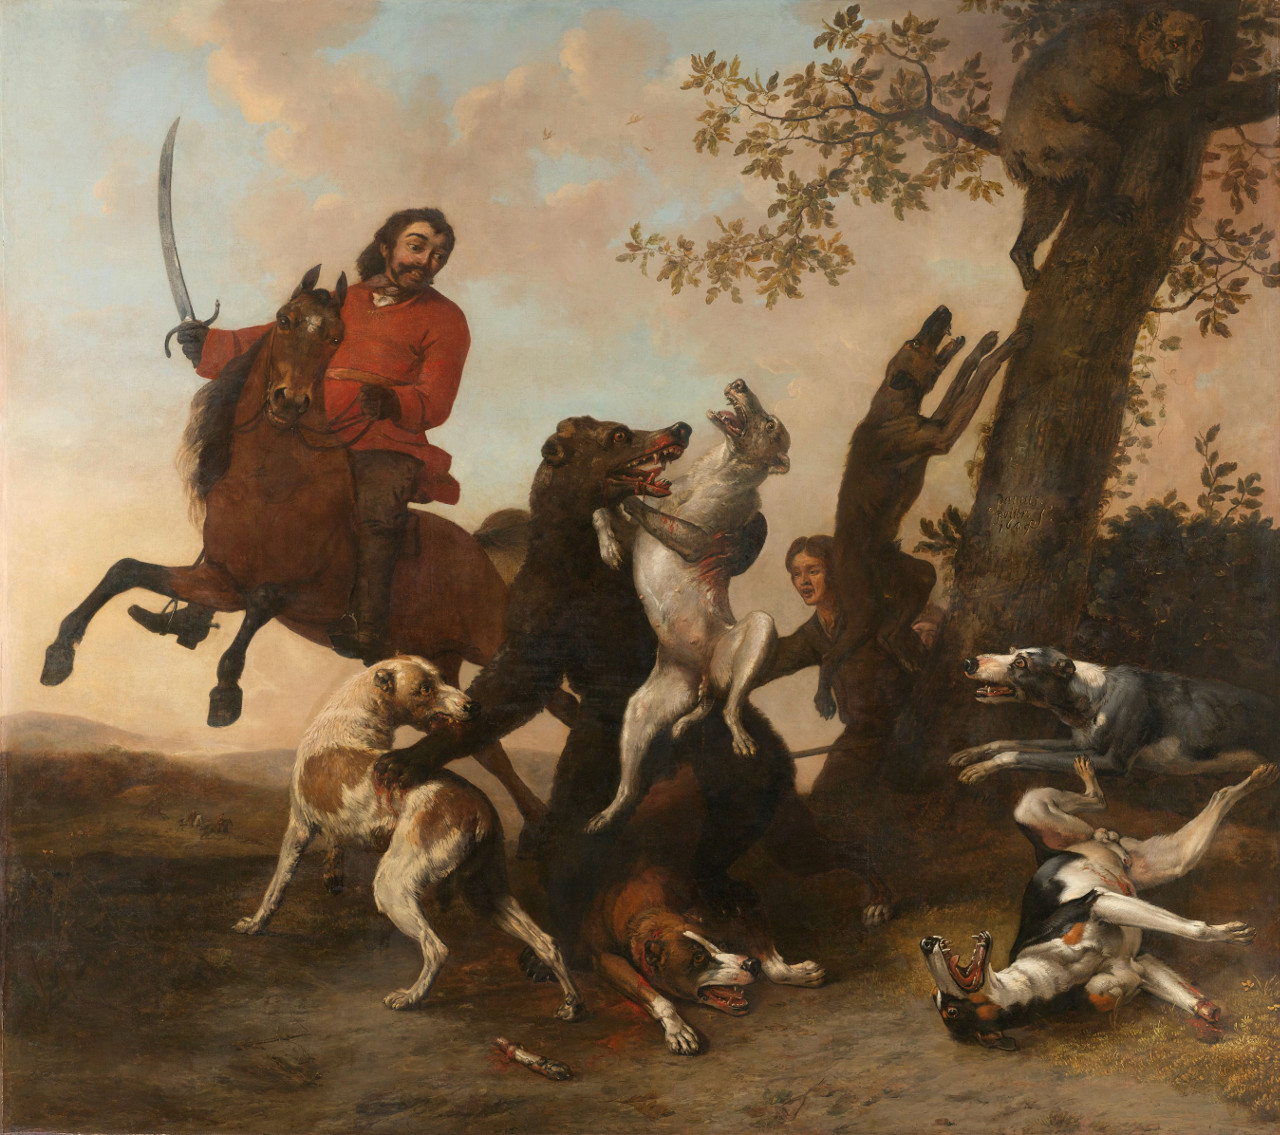
\includegraphics[width=\textwidth]{img/bear_hunt.jpg}
\captionsetup{labelformat=empty}
\caption{\small{
Паулюс Поттер. \urlnote{Медвежья охота}
{https://www.rijksmuseum.nl/en/collection/SK-A-316}.
1649 г. Государственный музей, Амстердам.
}}
\end{figure}
\setcounter{figure}{0}

\subsection{CAPM для оценки успеха управляющих}

Предположим, что вы дочитали до этого места и решили инвестировать свои средства 
в фондовый рынок. Есть несколько способов это сделать. Во-первых, вы можете 
сделать всё сами: открыть счёт у брокера, выбрать и купить конкретные акции, 
облигации или другие бумаги, а потом при необходимости перебалансировать свой 
портфель. Другой вариант --- принести деньги в \ruen{ПИФ --- паевой 
инвестиционный фонд}{mutual fund}, и тогда управляющий фондом сделает всё за 
вас.

Допустим, что вы выбрали способ инвестиций через ПИФ и теперь хотите понять, 
какой фонд обеспечит лучшее сочетание риска и доходности. Хоть прошлая 
доходность и не гарантирует успехов в будущем, всё равно имеет смысл посмотреть, 
какой доход получили другие инвесторы этого фонда.

Чтобы пример был жизненным, я собрал данные о доходности трёх российских ПИФов 
акций с ноября 2015-го года по сентябрь 2020-го. Назовём эти фонды <<красный>>, 
<<жёлтый>> и <<зелёный>>. Ноябрь 2015-го выбран не случайно, потому что именно 
тогда я сформировал свой собственный портфель акций на Московской бирже. Так что 
к сравнению трёх ПИФов можно добавить и фонд под кодовым названием <<автор>>.

Выяснилось, что за пять лет красный фонд заработал для своих клиентов 104\%, 
жёлтый заработал 85\%, а зелёный 84\%. Портфель автора вырос на 100\%. Стоит ли 
похвалить управляющих фондов? Будет ли довольна супруга автора, когда он будет 
хвастаться результатами?

Поскольку моя супруга училась на том же факультете, что и я, и не менее въедливо 
смотрит на цифры, то наверняка она задаст мне несколько вопросов. Во-первых, 
сколько бы мы заработали, если бы держали деньги на депозите (в безрисковом 
активе)? Во-вторых, на сколько за это время вырос весь рынок акций? В третьих, и 
в-главных, какой риск мы на себя взяли и какое соотношение риска и доходности 
получили?

На первые два вопроса ответить нетрудно. За рассматриваемый период индекс  
полной доходности МосБиржи (плюс дивиденды минус налоги) вырос на 217\%. 
Ключевая ставка ЦБ, которую я взял как приближение безрисковой ставки, дала бы 
50\%. На рисунке \ref{fund_total_growth_figure} представлены результаты фондов, 
индекса и безрисковой ставки.

\begin{figure}[h]
\centering
\begin{tikzpicture}
\begin{axis}[
    width=\textwidth,
    date coordinates in=x,
    date ZERO=2015-10-31,
    xtick={2016-01-01,2017-01-01,2018-01-01,2019-01-01,2020-01-01},
    xticklabel=\year,
    xmin=2015-10-31,
    xmax=2021-01-01,
    grid=major,
    ylabel={Рост 1 р. начальных инвестиций},
    legend entries = {
        Индекс МосБиржи,
        Ставка ЦБ,
        Автор,
        Красный,
        Жёлтый,
        Зелёный
    },
    legend pos=north west,
    legend style={font=\small},
    legend cell align={left}
]

    \newcommand{\addFundPlot}[4]{
        \addplot[
            color = #2,
            mark = #3, 
            style = #4,
            line width = 1pt,
            mark repeat = 4,
            mark phase = 3
        ]
        table[
            x = date,
            y = #1,
            col sep = comma
        ]
        {data/fund_growth.csv};
    }
    
    \addFundPlot{benchmark_growth}{Set1-D}{none}{solid}
    \addFundPlot{risk_free_growth}{Set1-D}{none}{dashed}
    \addFundPlot{personal_growth}{Set1-B}{o}{solid}
    \addFundPlot{red_growth}{Set1-A}{*}{solid}
    \addFundPlot{yellow_growth}{Set1-E}{square}{solid}
    \addFundPlot{green_growth}{Set1-C}{square*}{solid}
\end{axis}
\end{tikzpicture}

\caption{Доходности фондов, индекса и безрисковой процентной ставки.}
\label{fund_total_growth_figure}
\end{figure}

Чтобы ответить на третий вопрос о риске придётся потрудиться. Вспомним, что по 
CAPM средняя доходность любого актива (или портфеля активов) зависит только от 
<<беты>> и доходности рынка.
\begin{align*}
\underbrace{\mathbb{E}(R_{fund}) - R_{free}}_{\mathclap{\text{избыточная
доходность}}}
=
\beta_{fund} \underbrace{\left(\mathbb{E}(R_{mkt}) - R_{free}\right)}
_{\mathclap{\text{рыночная премия за риск}}}
\end{align*}

Как узнать <<бету>> фонда? Нет ничего проще. Сначала посмотрим на месячные 
доходности фонда $R_{fund,t}$ ($t$ --- номер месяца), индекса $R_{mkt,t}$ и 
безрискового актива $R_{free,t}$. Затем оценим следующую линейную регрессию 
(чуть ниже я поясню, что это такое, если вы не в курсе или забыли):
\begin{align}
R_{fund,t} - R_{free,t} = \alpha + \beta(R_{mkt,t} - R_{free,t}) + \epsilon,
\quad \epsilon_t \sim \mathcal{N}(0, \sigma_{\epsilon}^2)
\label{capm_regression}
\end{align}

Объяснить суть линейной регрессии на пальцах проще всего графически. Посмотрите 
на рисунок \ref{fund_regression_figure}. На оси $x$ отложены месячные доходности 
индекса сверх безрисковой ставки. На оси $y$ --- месячные избыточные доходности 
красного фонда (красные квадратики) и портфеля автора (синие кружки). Например, 
если вы видите красненький квадратик с координатами $(7.9\%, 9.7\%)$, то был 
месяц (январь 2018-го года, если это важно), когда индекс вырос на 7.9\% выше 
безрисковой процентной ставки, а красный фонд --- на 9.7\%.

\begin{figure}[h]
\centering
\begin{tikzpicture}
\begin{axis}[
    width=\textwidth,
    legend entries = {
        Автор,
        Красный фонд,
        $y = 0.12 + 0.60x$,
        $y = -0.05 + 0.92x$
    },
    legend pos=north west,
    legend style={font=\small},
    legend cell align={left},
    xlabel={Месячная избыточная доходность индекса, \%},
    ylabel={Месячная избыточная доходность фонда, \%},
    grid=major,
    xmin=-11,xmax=11,
    ymin=-11,ymax=11
]

    \newcommand{\addReturnPoints}[3]{
        \addplot[
            color = #2,
            mark = #3,
            only marks,
            mark size = 3pt
        ]
        table[
            x = benchmark_excess_return,
            y = #1,
            col sep = comma
        ]
        {data/fund_excess_return.csv};
    }
    
    \newcommand{\addRegressionLine}[3]{
        \addplot[
            color = #3,
            domain = -12:12,
            line width = 1pt
        ]
        {#1 + #2*x};
    }
    
    \addReturnPoints{personal_excess_return}{Set1-B}{*}
    
    \addReturnPoints{red_excess_return}{Set1-A}{square*}

    \addRegressionLine{0.1163}{0.5995}{Set1-B}

    \addRegressionLine{-0.04577}{0.9202}{Set1-A}
\end{axis}
\end{tikzpicture}
\caption{Связь доходностей фондов с доходностью индекса.}
\label{fund_regression_figure}
\end{figure}

Невооружённым глазом видна зависимость: в те месяцы, когда индекс показывает 
рост, портфели фондов тоже растут. Когда индекс падает, портфели фондов тоже 
обычно падают.

Чтобы выразить это наблюдение численно, можно задать следующий вопрос. 
Предположим, что доходность красного фонда связана с доходностью индекса простым 
линейным соотношением $y = \alpha + \beta x$. Какие коэффициенты $\alpha$ и 
$\beta$ нужно подставить в это уравнение прямой, чтобы прямая проходила <<ближе 
всего>> ко всем красным квадратикам на графике? Ответ: лучше всего подойдёт 
прямая $y = -0.05 + 0.92x$, то есть $\alpha = -0.05$ и $\beta=0.92$.

Поздравляю, вы только что построили линейную регрессию методом \ruen{наименьших 
квадратов}{ordinary least squares, OLS}! За деталями того, каким алгоритмом 
можно вычислить эти коэффициенты, отсылаю вас к любому учебнику эконометрики, 
например \cite[ch.~2]{verbeek2012guide}. Если решить аналогичную задачу и для 
остальных фондов, то получится таблица \ref{capm_regression_results}.

\begin{table}[h]
\centering
\begin{tabular}{l|r|r|r|r|r}
\multirow{2}{*}{Фонд} & 
\multirow{2}{*}{$\hat{\alpha}$ (ст. откл.)} &
\multirow{2}{*}{$\hat{\beta}$ (ст. откл.)}  &
\multirow{2}{*}{$R^2$} &
Отнош.&
Отнош. \\
& & & & Шарпа & Сортино \\ \hline
Автор   &  0.12\% (0.29\%) & 0.60 (0.07) & 0.54 & 0.60 & 1.08 \\
Красный & -0.05\% (0.18\%) & 0.92 (0.05) & 0.87 & 0.55 & 0.90 \\
Жёлтый  & -0.20\% (0.26\%) & 0.91 (0.07) & 0.75 & 0.38 & 0.62 \\
Зелёный & -0.28\% (0.16\%) & 1.00 (0.04) & 0.91 & 0.37 & 0.58 \\ \hline
Индекс  &  0.00\% (0.00\%) & 1.00 (0.00) & 1.00 & 0.64 & 1.02
\end{tabular}
\caption{Регрессия избыточных доходностей фондов на избыточную доходность 
индекса. 59 месячных наблюдений 11.2015--09.2020. Значения $\hat{\alpha}$ и 
$\hat{\beta}$ для месячных доходностей. Отношения Шарпа и Сортино 
сконвертированы в годовое выражение умножением на $\sqrt{12}$.}
\label{capm_regression_results}
\end{table}

Как интерпретировать таблицу \ref{capm_regression_results}? Начнём с <<беты>>. 
Например, <<бета>> красного фонда оказалась равной 0.92. Это наша оценка 
<<беты>> красного фонда по CAPM. В среднем, когда весь рынок (индекс) давал 
избыточную доходность выше безрисковой ставки 1\%, красный фонд давал избыточную 
доходность 0.92\%. Это мера систематического рыночного риска, который взял 
управляющий красным фондом.

Теперь посмотрим на <<альфу>>. По CAPM, никакой <<альфы>> нет и быть не может, 
потому что доходность фонда зависит исключительно от <<беты>> и доходности 
рынка. Если какой-то фонд имеет положительную <<альфу>>, то фонд зарабатывает 
больше, чем можно было бы ожидать при том же уровне систематического рыночного 
риска. Если <<альфа>> отрицательная, то вкладчики фонда получают меньшую 
компенсацию за систематический риск, чем можно было бы ждать по CAPM.

Интересно, что во всех трёх ПИФах <<альфа>> оказалась отрицательной. А вот 
портфель автора обогнал CAPM и зарабатывал дополнительные 0.12\% в месяц сверх 
ожидаемой рыночной премии за риск. Кому-то может показаться, что 0.12\% это 
копейки. Возражу, что 0.12\% в месяц --- это почти 1.5\% дополнительной 
доходности в год, что совсем неплохо. Да и в конце концов, пусть <<альфа>> 
маленькая, зато своя!

Скептик возразит, что при стандартном отклонении 0.29\% значение <<альфы>> 
0.12\% статистически не отличается от нуля. Это правда, и с этим невозможно 
спорить. Такова реальность финансовых рынков. Зачастую у вас нет достаточно 
длинной истории наблюдений, чтобы получить статистически значимые оценки. Если 
подождать ещё лет 15 и накопить побольше данных, то, быть может, получится 
подтвердить, что <<альфа>> автора статистически значима. Но принимать 
инвестиционное решение и выбирать фонд вам нужно сейчас, а не через 15 лет! Так 
что придётся смотреть на те данные, что у нас есть.

Ещё один интересный параметр, который выдаёт линейная регрессия --- это $R^2$, 
он же \ruen{эр-квадрат}{R-squared}. $R^2$ принимает значения от 0 до 1. 
Неформально, это доля дисперсии (колебаний) доходности фонда, которую можно 
объяснить линейной моделью. Ещё более неформально, $R^2$ показывает, насколько 
хорошо прямые линии с рисунка \ref{fund_regression_figure} приближают облако 
точек.

Например, регрессия для зелёного фонда показала $R^2$ 0.91. Можно 
интерпретировать это так, что 91\% колебаний доходности зелёного фонда 
объясняется колебаниями доходности рынка, и только 9\% --- действиями 
управляющего. Вместе с <<бетой>> около единички и отрицательной <<альфой>> это 
создаёт не самую хорошую картину. Вкладчики зелёного фонда взяли на себя тот же 
систематический риск, что и в индексе, но при этом недополучили премию за риск 
на 3.3\% в год. 

Сложно сказать, связан ли такой результат зелёного фонда с высокой комиссией за 
управление или с конкретными инвестиционными решениями управляющего. Но если бы 
клиенты зелёного фонда могли купить все акции в индексе МосБиржи, то они 
получили бы доходность на 3\% годовых выше при том же уровне систематического 
риска. Запомним эту мысль.

\subsection{Факторные портфели}

Что ни говори, результат авторского портфеля из таблицы 
\ref{capm_regression_results} выглядит подозрительно. Положительная <<альфа>>. 
Относительно невысокая <<бета>> (чувствительность к систематическому рыночному 
риску). А главное, $R^2$ в районе 0.5, то есть только половину колебаний 
портфеля автора можно связать с движениями всего рынка.

Нет ли здесь подвоха? Да, в рамках CAPM единственный риск, за который можно 
заработать премию --- это систематический рыночный риск. Да, движения рынка 
неплохо объясняют колебания портфеля автора. Но что если CAPM говорит нам не всю 
правду, и на рынке есть другие систематические риски, за которые можно 
заработать премию за риск? Вдруг автор сделал ставку на такой риск, который не 
входит CAPM, и именно этим объясняется его мнимый успех? Стоит разобраться в 
этом вопросе прежде чем вставать в очередь желающих доверить автору деньги в 
управление.

Довольно давно исследователи заметили на рынке акций США аномалии, которые 
нельзя объяснить CAPM. Вот некоторые из них.

Во-первых, \ruen{эффект размера}{size effect}. Замечено, что акции маленьких 
компаний растут лучше, чем акции крупных компаний (разумеется, при одинаковой 
<<бете>>).

Во-вторых, \ruen{эффект стоимости}{value effect}. Для каждой компании можно 
посчитать две разных стоимости. Первая --- \ruen{рыночная стоимость}{market 
value}, то есть рыночная цена одной акции, умноженная на количество акций. 
Вторая --- \ruen{бухгалтерская стоимость}{book value}, то есть оценка 
акционерного капитала из финансовой отчётности. Все акции на рынке можно грубо 
разделить на акции стоимости (компании с высоким отношением book value / market 
value) и акции роста (компании с низким отношением book value / market value).

Заезженный пример компании стоимости --- коммунальные сети с понятными 
физическими активами. Не менее заезженный пример компании роста --- интернет-
гигант, у которого значительная часть активов нематериальна и не отражена в 
бухгалтерском балансе. Так вот, эффект стоимости заключается в том, что акции 
стоимости приносят более высокую доходность, чем акции роста (опять же, при 
равной <<бете>>).

В-третьих, \ruen{эффект инерции}{momentum effect}. Оказывается, что акции, 
которые выросли в прошлом году, с большей вероятностью будут расти и в этом. С 
другой стороны, акции, упавшие в прошлом году, с большей вероятностью продолжат 
падать и в этом.

Чтобы оценить эти эффекты численно, \ruen{Юджин Фама}{Eugene Fama} и 
\ruen{Кеннет Френч}{Kenneth French} предложили составить так называемые 
\ruen{факторные портфели}{factor portfolios}. Факторный портфель это такая 
комбинация из купленных и проданных в короткую акций, которая зарабатывает 
деньги за счёт одного их перечисленных эффектов. Проще всего объяснить на 
примерах.

Чтобы составить портфель \en{SMB (Small Minus Big)}, инвестор должен 
отсортировать все компании на рынке по размеру (рыночной капитализации) и  
разделить список пополам. В одной половине окажутся акции, которые мы назовём 
маленькими, а во второй окажутся акции, которые мы назовём большими. Осталось 
купить по списку все маленькие акции и продать в короткую все большие. Если 
эффект размера существует, то купленные маленькие акции принесут больший доход, 
чем проданные большие акции.

Для портфеля \en{HML (High book/market Minus Low book/market)}\ нужно 
отсортировать компании по отношению \en{book/value}, то есть бухгалтерского 
капитала к рыночной капитализации. После этого нужно купить треть акций с самым 
высоким отношением book/market (акций стоимости) и продать в короткую треть 
акций с низким отношением book/market (акций роста). Если мы правы насчёт 
эффекта стоимости, то акции стоимости обгонят акции роста, и портфель принесёт 
прибыль.

Аналогично, для портфеля \en{MOM (MOMentum)}\ нужно купить 30\% лучших акций 
прошлого года и продать в короткую 30\% худших. Опять-таки, портфель будет 
зарабатывать деньги, если эффект инерции работает, и прошлогодние победители 
действительно обгонят прошлогодних проигравших.

Строго говоря, процедура построения портфелей SMB, HML и MOM чуточку сложнее, 
чем я описал. Однако, это технические детали, которые только запутают изложения. 
Подробности можно посмотреть, например, в книге \cite[ch.~9--11]
{bali2016empirical} или на уже упоминавшемся сайте профессора Френча 
\cite{kennethFrench}.

Как бы то ни было, у нас есть портфели из акций, которые могут заработать нам 
деньги за счёт эффектов размера, стоимости и инерции. Чтобы составить эти 
портфели, достаточно уметь сортировать акции по простому критерию и делить
отсортированный список на части. Почти как в анекдоте --- сортируй и дели! С 
этой задачей справится и пятилетний ребёнок, и компьютер. Было бы странно, если 
бы настолько бездумно и механически составленные портфели давали положительную 
доходность, не так ли?

Как бы не так! На рисунке \ref{us_factor_returns_figure} и в таблице 
\ref{us_factor_returns_table} представлены исторические доходности трёх 
факторных портфелей на рынке США. Как видите, на дистанции 94-х лет все три 
портфеля дали рост. Интерес к эффектам размера, стоимости и инерции возник не на 
пустом месте.

\begin{figure}[h]
    \begin{tikzpicture}
    \begin{axis}[
        width=\textwidth,
        date coordinates in=x,
        date ZERO=1926-06-30,
        xtick={1930-01-01,1940-01-01,1950-01-01,1960-01-01,1970-01-01,1980-01-01,1990-01-01,2000-01-01,2010-01-01,2020-01-01},
        minor xtick={1930-01-01,1950-01-01,1970-01-01,1990-01-01,2010-01-01},
        xticklabel=\year,
        grid=both,
        xmin=1926-12-31,
        xmax=2025-01-01,
        ymode=log,
        ymax=1000,
        log ticks with fixed point,
        ylabel={Рост \dollars{1} начальных инвестиций},
        legend entries={
            MOM (MOMentum),
            HML (High book/market Minus Low book/market),
            SMB (Small Minus Big)
        },
        legend pos=north west,
        legend style={font=\small},
        legend cell align={left}
    ]
    
    \newcommand{\addFactorPlot}[3]{
        \addplot[
            color=#2,
            mark=#3,
            line width=1pt,
            mark repeat=120,
            mark phase=36,
            mark options={scale=2}
        ]
        table [
            x = date,
            y = #1,
            col sep=comma
        ]
        {data/fama_french_cumulative_growth_data.csv};
    }

    \addFactorPlot{mom}{Set1-A}{o}

    \addFactorPlot{hml}{Set1-B}{square}
    
    \addFactorPlot{smb}{Set1-C}{diamond}

    \end{axis}
    \end{tikzpicture}
    \caption{
        Историческая доходность факторных портфелей.
        Данные: \cite{kennethFrench}.
    }
    \label{us_factor_returns_figure}
\end{figure}

\begin{table}[h]
\centering
\begin{tabular}{l|l|r|r|r|r|c}
Фактор & Период & Сред. & Ст. откл. & $t$-тест & $p$-знач. & 99\% дов. инт. \\
\hline
SMB & 1927--1959 &  3.4\% & 13.6\% & 1.41 & 16.7\% & [-1.5\%, 8.2\%] \\
    & 1960--1989 &  3.3\% & 13.9\% & 1.29 & 20.9\% & [-1.9\%, 8.4\%] \\
    & 1990--2020 &  0.8\% & 9.2\%  & 0.49 & 62.7\% & [-2.6\%, 4.2\%] \\
    & 1960--2020 &  2.0\% & 11.7\% & 1.34 & 18.4\% & [-1.0\%, 5.0\%] \\
    & 1927--2020 &  2.5\% & 12.4\% & 1.95 &  5.4\% & [-0.0\%, 5.0\%] \\ \hline

HML & 1927--1959 &  5.1\% & 14.1\% & 2.07 &  4.7\% & [0.1\%, 10.0\%] \\
    & 1960--1989 &  6.1\% & 11.1\% & 3.03 &  0.5\% & [2.0\%, 10.3\%] \\
    & 1990--2020 &  1.2\% & 15.3\% & 0.42 & 67.7\% & [-4.5\%, 6.8\%] \\
    & 1960--2020 &  3.6\% & 13.5\% & 2.08 &  4.1\% & [0.1\%, 7.1\%]  \\
    & 1927--2020 &  4.1\% & 13.7\% & 2.92 &  0.4\% & [1.3\%, 6.9\%]  \\ \hline
  
MOM & 1927--1959 &  7.4\% & 17.8\% & 2.40 &  2.3\% & [1.1\%, 13.7\%] \\
    & 1960--1989 & 10.5\% & 12.8\% & 4.49 & <0.1\% & [5.7\%, 15.2\%] \\
    & 1990--2020 &  6.6\% & 16.4\% & 2.24 &  3.3\% & [0.6\%, 12.6\%] \\
    & 1960--2020 &  8.5\% & 14.7\% & 4.50 & <0.1\% & [4.7\%, 12.3\%] \\
    & 1927--2020 &  8.1\% & 15.8\% & 4.98 & <0.1\% & [4.9\%, 11.4\%] \\
\end{tabular}
\caption{Годовые доходности факторных портфелей, 1927--2020. Данные: 
\cite{kennethFrench}.}
\label{us_factor_returns_table}
\end{table}

Что можно сказать о таблице \ref{us_factor_returns_table} помимо того, что за 
столетие факторные портфели приносили доход?

Во-первых, мы не можем отвергнуть гипотезу, что на самом деле портфель SMB 
(маленькие компании против больших) имеет нулевую доходность. Справедливости 
ради, до начала 1990-х, когда Фама и Френч опубликовали свою известную работу 
\cite{Fama93commonrisk}, доходность портфеля SMB была статистически значимой на 
уровне значимости 95\%. В последние же 30 лет портфель SMB растёт (средняя 
доходность положительная), но этот рост настолько волатильный, что мы не можем 
уверенно утверждать, что положительная доходность это не случайность. Решайте 
сами, что это значит для эффекта размера.

Во-вторых, в период 1990--2020 доходность всех трёх портфелей оказалась ниже, 
чем в среднем в истории. Возможно, это просто совпадение. Возможно, слишком 
много людей прочитали работы Фамы-Френча о факторах HML и SMB, а также Кархарта 
о факторе MOM \cite{carhart1997persistence}. В результате, например, спрос на 
маленькие акции в портфеле SMB вырос, из-за чего выросла их цена и снизилась 
ожидаемая доходность.

Возможно, что-то фундаментально изменилось. Например, мы вошли в эпоху IT-
гигантов, которые все как на подбор относятся к компаниям роста из-за 
околонулевой бухгалтерской стоимости нематериальных активов. Поэтому мы видим 
снижение доходности фактора HML, в который эти IT-гиганты входят со знаком 
<<минус>>. Сложно сказать, какое объяснение верное. Напомните мне вернуться к 
этому вопросу в 2050-м году.

Напоследок ещё пара замечаний о факторных портфелях.

Во-первых, факторные портфели имеют (точнее, имели в прошлом) положительную 
доходность только в среднем. Нет гарантии, что акции стоимости будут обгонять 
акции роста каждый год. Вполне может оказаться, что в какой-то год маленькие 
компании проиграют большим, акции стоимости проиграют акциям роста, прошлогодние 
победители проиграют прошлогодним проигравшим. Не стоит рассматривать факторные 
портфели как машинку для зарабатывания денег без риска.

Во-вторых, факторные портфели это скорее теоретическая конструкция, чем реальная 
инвестиционная стратегия. Чтобы сделать ставку, скажем, на портфель SMB, вам 
нужно продать в короткую большие акции, которых у вас нет, а на вырученные 
деньги купить маленькие акции. В теории, такой портфель не требует никаких 
начальных инвестиций, и его можно собрать по щелчку пальцев, не потратив ни 
цента.

На практике, брокеры, конечно, предоставляют своим клиентам услугу коротких 
продаж (когда брокер берёт взаймы акцию у другого клиента и одалживает её вам). 
Однако, эта услуга отнюдь не бесплатная и распространяется далеко не на все 
акции. Вдобавок, многим инвесторам, таким как паевые фонды, короткие продажи 
просто-напросто запрещены законом.

Так что я с трудом представляю себе управляющего фондом, который в реальной 
жизни собрал бы портфель SMB. Впрочем, практическая ценность SMB и других 
портфелей не в этом. В чём --- читайте дальше.

\subsection{Многофакторная модель для оценки успеха управляющих}

Итак, у нас есть три портфеля, SMB, HML и MOM. Предположим, что они на самом 
деле имеют положительную ожидаемую доходность. Как примирить это с нашей идеей, 
что заработать премию можно только за систематический риск? Нет ничего проще. 
Нужно постановить, что факторные портфели отвечают за иные виды систематического 
риска, не связанные с систематическим рыночным риском из CAPM.

Если бы мы занимались теоретической наукой, то нам пришлось бы искать 
объяснение, \emph{почему} рациональные инвесторы с какой-то там функцией 
полезности требуют и получают премию за риск, например, компаний стоимости и 
портфеля HML. Это, конечно, важно для науки, но не столь важно для нашей задачи 
оценки управляющих. Здесь мне близок подход некоторых физиков к квантовой 
механике: \ruen{<<Заткнись и считай!>>}{<<Shut up and calculate!>>}. Я не знаю, 
какой риск изображают факторные портфели, но это не мешает мне использовать их 
для расчётов.

Вспомним линейную регрессию (\ref{capm_regression}), по которой мы оценивали 
доходность фондов. Дополним её ещё несколькими объясняющими переменными. А 
именно, для каждого периода $t$ посчитаем гипотетические доходности портфелей 
SMB, HML и MOM --- $R_{smb,t}$, $R_{hml,t}$ и $R_{mom,t}$ соответственно. Тогда 
у нас получится регрессия, которую называют четырёхфакторной моделью Фамы-
Френча-Кархарта:
\begin{align}
\nonumber
R_{fund,t} - R_{free,t} &= \alpha
+ \beta_{mkt}\left(R_{mkt,t} - R_{free,t}\right) 
+ \beta_{smb}R_{smb,t} + \\
&+ \beta_{hml}R_{hml,t}
+ \beta_{mom}R_{mom,t}
+ \epsilon_t,
\quad
\epsilon_t \sim \mathcal{N}(0, \sigma_{\epsilon}^2)
\label{four_factor_regression}
\end{align}

Идея ровно та же, что и в предыдущей регрессии. Мы хотим посмотреть, как 
доходность фонда связана с доходностями четырёх факторных портфелей: уже 
знакомого нам рыночного портфеля из CAPM (который мы приближаем индексом акций) 
и трёх новых факторных портфелей SMB, HML и MOM.

Например, если мы вычислим, что $\hat{\beta}_{smb} > 0$, то это означает, что 
управляющий фонда сделал ставку на эффект размера. Конечно, вряд ли он собрал 
портфель SMB в чистом виде (как я говорил, это крайне сложно сделать на 
практике). Скорее всего, он купил в портфель больше маленьких акций, чем 
больших. Поэтому в те периоды, когда портфель SMB показывал рост, портфель 
управляющего тоже показывал дополнительный рост относительно CAPM.

Коэффициент $\beta_{smb}$ имеет тот же смысл, что и обычная <<бета>> к рынку 
$\beta_{mkt}$. Скажем, если $\beta_{smb}=1.5$, то при росте портфеля SMB на 1\% 
(маленькие акции в среднем выросли на 1\% выше, чем большие) портфель 
управляющего при прочих равных растёт на 1.5\%. Если портфель SMB падает на 1\% 
(маленькие акции отстали от больших на 1\%), то при прочих равных портфель фонда 
теряет 1.5\%.

Говоря ещё проще, все четыре <<беты>> из регрессии 
(\ref{four_factor_regression}) показывают, какой систематический риск (или 
риски) взял на себя управляющий фондом. <<Альфа>> говорит, заработал ли он что-
то сверх премии за эти систематические риски. Положительная <<альфа>> в 
четырёхфакторной модели означает, что управляющий фондом делает что-то ещё 
помимо ставок на рост рынка и эффекты размера, стоимости и инерции.

Плохая новость: согласно ещё одной известной работе Фамы и Френча 
\cite{fama2010luck}, средняя <<альфа>> американских паевых фондов по 
четырёхфакторной модели составляет -1.1\% в год после вычета комиссий. К 
сожалению, средний инвестор в паевой фонд получает меньшую компенсацию за 
систематический риск, чем мог бы.

Готов поспорить, что вам теперь не терпится проверить на прочность положительную 
<<альфу>> автора статьи, прогнав её через четырёхфакторную модель. Вполне 
понимаю ваше желание. Впрочем, зная цифры, я предпочту оттянуть бесславный конец 
и вставлю в статью ещё один занудный теоретический раздел.

\subsection{Арбитражная теория ценообразования (APT)}

Почему вообще мы решили записать многофакторную регрессию 
(\ref{four_factor_regression})? Если помните, за однофакторной регрессией 
\ref{capm_regression} стояла стройная теория CAPM (ну, я по крайней мере 
попытался стройно её описать). Эта теория гласит, что избыточная доходность 
любого портфеля \emph{должна} быть пропорциональна избыточной доходности рынка.

Есть ли теоретические соображения за четырёхфакторной регрессией, которые бы 
объясняли, почему доходность портфеля должна зависеть от SMB? Ведь если их нет, 
то не занимаемся ли мы \ruen{дата майнингом}{data mining}, бездумно закидывая в 
топку линейной регрессии всё больше объясняющих переменных?

Такое теоретическое объяснение есть, и оно называется \ruen{арбитражная теория 
ценообразования}{arbitrage pricing theory, APT}.

В чём суть APT? На рынке всегда есть участники, которые называются 
\ruen{арбитражёрами}{arbitrageurs}. Арбитражёры пристально следят за тем, чтобы 
цены не выходили из равновесия. Если они видят, что акция A безосновательно 
подешевела относительно акции B, то они купят акцию A и продадут акцию B, чтобы 
заработать на этом. При этом спрос на акцию A вырастет, как и её цена. 
Предложение акции B увеличится, и её рыночная цена упадёт. В результате ошибка 
рынка исчезнет, а арбитражёры заработают прибыль. Такая возможность заработать 
на ошибке рынка называется \ruen{арбитраж}{arbitrage}.

Поскольку по рынку всегда бродит множество алчных арбитражёров, которые 
выискивают малейшие ошибки рынка, то возможности для арбитража, если они и 
возникают, пропадают очень быстро. Согласно крылатой фразе, на рынке \ruen{нет 
бесплатных обедов}{there is no free lunch}.

Давайте я изложу этот аргумент чуть более формально, пользуясь идеей из книги 
\cite[p.~180]{cochrane2005asset}.

Предположим, что на рынке есть в общей сложности $n$ факторов систематического 
риска, за которые можно заработать премию за риск. Пусть у нас есть $n$ 
факторных портфелей $P_1,...,P_n$, каждый из которых изображает (proxy) один из 
этих факторов. Обозначим доходности этих портфелей (премии за риск)
$R_1,...,R_n$. Тогда ожидаемая доходность любого актива $R_{asset}$ должна быть 
равна
\begin{equation}
\mathbb{E}(R_{asset}) - R_{free} = 
\beta_1\mathbb{E}(R_1) + \beta_2\mathbb{E}(R_2) + ... + \beta_n\mathbb{E}(R_n)
\label{apt_equation}
\end{equation}

Предположим, что это не так, и существует актив с положительной <<альфой>> в 
регрессии:
\begin{equation}
R_{asset,t} - R_{free,t} = \alpha + 
\beta_1R_{1,t} + \beta_2R_{2,t} + ... + \beta_nR_{n,t} + \epsilon_t,
\quad
\epsilon_t \sim \mathcal{N}(0, \sigma_{\epsilon}^2)
\label{apt_regression_example}
\end{equation}

Что сделает алчный арбитражёр, наткнувшись на такую явную ошибку рынка? 
Разумеется, он сразу же купит этот актив и продаст все факторные портфели в 
количествах $\beta_1$, $\beta_2$ и так далее до $\beta_n$. Какую доходность $R$ 
он получит?
\begin{equation*}
R = R_{asset} - \beta_1R_{1} - \beta_2R_{2} - ... - \beta_nR_{n}
= R_{free} + \alpha + \epsilon
\end{equation*}

В правой части у нас сумма констант $\alpha$ и $R_{free}$ и случайной величины
$\epsilon$, которая является ошибкой регрессии (\ref{apt_regression_example}). 
Чем точнее факторные портфели приближают актив (чем лучше $R^2$ регрессии), тем 
меньше стандартное отклонение ошибки регрессии $\sigma_{\epsilon}$, то есть 
меньше риск арбитражёра. С другой стороны, чем больше $\alpha$, тем выше его 
потенциальная доходность.

Получается, что чем больше ошибка рынка, и чем лучше факторные портфели 
приближают актив, тем лучшее соотношение доходности и стандартного отклонения 
(отношение Шарпа) получит арбитражёр. Арбитражёр никогда не пройдёт мимо ошибки 
рынка, которая обещает прибыль с хорошим отношением Шарпа. Если цены сильно 
отклонятся от равновесия (\ref{apt_equation}), то арбитражёры тут же налетят как 
коршуны и исправят это недоразумение.

Как видите, APT исходит из иных предпосылок нежели CAPM. В CAPM мы выводили 
доходности активов исходя из свойств рациональных инвесторов. В APT мы 
сравниваем активы друг с другом и говорим, что активы с одинаковой доходностью 
(актив с одной стороны и комбинация факторных портфелей с другой) не могут 
стоить разных денег. Это называется \ruen{закон одной цены}{law of one price}. 

Можно ещё сказать, что APT оценивает активы друг относительно друга, а не в 
абсолютном выражении. Например, APT говорит, что два сорта нефти, Brent и WTI 
должны стоить более-менее одинаковых денег. Не должно быть такого, что WTI стоит 
\dollars{100} за баррель, а Brent всего \dollars{10}. Однако APT не говорит, 
сколько должен стоить баррель нефти: \dollars{10} или \dollars{100}.

С точки зрения практики, в APT можно добавить почти сколько угодно факторов 
риска. Главное, чтобы факторы были представлены портфелями торгуемых активов. У 
управляющего фондом должна быть хотя бы гипотетическая возможность купить 
факторный портфель. Факторы размера (SMB), ценности (HML) и инерции (MOM) 
удовлетворяют этому правилу. А вот, скажем, фактор <<средняя температура 
января>> --- нет, хотя он и может влиять на цены акций энергетических компаний.

Стоит отметить, что хоть мы и рассматривали, в основном, акции, идеи APT и 
факторного анализа доходности можно применить и к другим классам активов. 
Например, если вы оцениваете результаты управляющего фондом облигаций, то вам 
нужно выбрать соответствующие факторы.

Во-первых, вам нужно будет выбрать релевантный индекс облигаций. Во-вторых, 
неплохо добавить в регрессию факторы, основанные на форме кривой доходности и 
кредитном рейтинге. Скажем, за форму кривой доходности будет отвечать портфель 
<<десятилетние облигации минус годовые облигации>>, а за кредитный рейтинг --- 
портфель <<облигации с рейтингом BBB минус облигации с рейтингом AAA>>.

В целом, человечество придумало сотни, если не тысячи, факторных портфелей, 
которые можно применить в той или иной ситуации. Это чрезвычайно полезно, когда 
вы хотите понять, какой риск вы (или ваш управляющий) взяли на себя.

Согласно одной из радикальных точек зрения, никакой <<альфы>> на самом деле нет, 
а есть только <<беты>>, которые мы не видим. Если кто-то заработал <<альфу>>, то 
есть доход, превышающий предсказание модели, то первым делом стоит проверить, а 
не скрывается ли за этой <<альфой>> какая-то <<бета>>. Вдруг управляющий взял на 
себя неизвестный нам систематический риск, и звёзды так сошлись, что в отчётном 
периоде премия за этот риск оказалась положительной?

\subsection{Факторные портфели на российском рынке}

Что ж, сколько верёвочке ни виться, а пересчитать <<альфу>> автора всё равно 
придётся. Для этого нам будут нужны факторные портфели, составленные из 
российских акций. Исследователи из ИПЭИ РАНХиГС проделали титаническую работу по 
сбору и подготовке данных и выложили на сайте <<Конструктор CAPM-RU>> 
\cite{capmruWeb}  временные ряды нескольких факторных портфелей.

\begin{enumerate}
\setlength{\itemsep}{0pt}
\item MKT-RF --- доходность рынка минус безрисковая процентная ставка, как в 
CAPM.
\item SMB --- маленькие акции минус большие акции, как у Фамы-Френча.
\item HML --- акции стоимости минус акции роста, как у Фамы-Френча.
\item MOM --- прошлогодние победители минус прошлогодние проигравшие, как у 
Кархарта (на момент написания статьи недоступен по техническим причинам).
\item LIQ (LIQuidity) --- неликвидные акции минус ликвидные. Если этот портфель 
даёт положительную доходность, то на рынке есть премия за риск за владение 
неликвидными акциями.
\item DY (Dividend Yield) --- акции с высокой дивидендной доходностью 
(отношением дивиденды/цена) минус акции с низкой дивидендной доходностью. Если 
доходность этого портфеля положительная, то инвесторы в <<дивидендные>> акции в 
среднем зарабатывают больше.
\item SOE (State-Owned Enterprise) --- акции частных компаний минус акции 
компаний с государственным участием. Если доходность этого портфеля 
положительная, то акции частных компаний дают большую доходность, чем акции 
государственных компаний.
\end{enumerate}

На рисунке \ref{ru_factors_figure_2005} изображены доходности шести факторных 
портфелей (минус фактор MOM, для которого по техническим причинам нет данных) с 
2005-го года. Рисунок \ref{ru_factors_figure_2015} показывает те же факторы за 
период с 2015-го года на случай, если вы не без оснований опасаетесь, что 
российский рынок середины 2000-х и конца 2010-х это две большие разницы. 
Наконец, в таблице \ref{ru_factor_stats} я посчитал средние, стандартные 
отклонения и доверительные интервалы доходностей.

\begin{figure}[h]
\centering
\begin{tikzpicture}
    \begin{axis}[
        width=\textwidth,
        date coordinates in=x,
        date ZERO=2004-12-31,
        xtick={2005-01-01,2008-01-01,2011-01-01,2014-01-01,2017-01-01,2020-01-01},
        xticklabel=\year,
        xmin=2005-01-01,
        xmax=2021-01-01,
        ymin=0,
        ymax=10,
        grid=major,
        ylabel={Рост 1 р. начальных инвестиций},
        legend entries = {
            MKT-RF,
            SMB,
            HML,
            LIQ,
            DY,
            SOE
        },
        legend pos=north west,
        legend style={font=\small},
        legend cell align={left}
    ]
    
    \newcommand{\addFactorPlot}[3]{
        \addplot[
            color = #2,
            mark = #3,
            line width = 1pt,
            mark repeat = 36, 
            mark phase = 36,
            mark options = {scale=2}
        ]
        table[
            x = month,
            y = #1,
            col sep = comma
        ]
        {data/ru_factors_cumulative_growth_data.csv};
    }
    
    \addFactorPlot{rmrf_ru}{Set1-A}{none}
    \addFactorPlot{smb_ru} {Set1-B}{o}
    \addFactorPlot{hml_ru} {Set1-C}{square}
    \addFactorPlot{liq_ru} {Set1-D}{triangle}
    \addFactorPlot{dy_ru}  {Set1-E}{oplus}
    \addFactorPlot{soe_ru} {Set1-G}{diamond}
    \end{axis}
    \end{tikzpicture}

    \caption{
        Доходность факторных портфелей на рынке акций России, 2005--2020.
        Данные:\cite{capmruWeb}.
    }
    \label{ru_factors_figure_2005}
\end{figure}

\begin{figure}[h]
    \centering
    \begin{tikzpicture}
    \begin{axis}[
        width=\textwidth,
        date coordinates in=x,
        date ZERO=2004-12-31,
        xtick={2015-01-01,2016-01-01,2017-01-01,2018-01-01,2019-01-01,2020-01-01},
        xticklabel=\year,
        xmin=2014-12-31,
        xmax=2020-06-01,
        ymin=0.5,
        ymax=2.5,
        grid=major,
        ylabel={Рост 1 р. начальных инвестиций},
        legend entries = {
            MKT-RF,
            SMB,
            HML,
            LIQ,
            DY,
            SOE
        },
        legend pos=north west,
        legend style={font=\small},
        legend cell align={left}
    ]
    
    \newcommand{\addFactorPlot}[3]{
        \addplot[
            color = #2,
            mark = #3,
            line width = 1pt,
            mark repeat = 12, 
            mark phase = 13,
            mark options = {scale=2}
        ]
        table[
            x = month,
            y = #1,
            col sep = comma
        ]
        {data/ru_factors_cumulative_growth_data_2015.csv};
    }
    
    \addFactorPlot{rmrf_ru}{Set1-A}{none}
    \addFactorPlot{smb_ru} {Set1-B}{o}
    \addFactorPlot{hml_ru} {Set1-C}{square}
    \addFactorPlot{liq_ru} {Set1-D}{triangle}
    \addFactorPlot{dy_ru}  {Set1-E}{oplus}
    \addFactorPlot{soe_ru} {Set1-G}{diamond}
    \end{axis}
    \end{tikzpicture}

    \caption{
        Доходность факторных портфелей на рынке акций России, 2015--2020.
        Данные: \cite{capmruWeb}
    }
    \label{ru_factors_figure_2015}
\end{figure}

\begin{table}[h]
\centering
\begin{tabular}{l|r|r|r|r|c}
Фактор & Среднее & Ст. откл. & $t$-тест & $p$-знач. & 99\% дов. инт. \\
\hline
MKT-RF & 0.93\% & 6.6\% & 1.90 &  5.9\% & [-0.0\%, 1.9\%] \\
SMB    & 1.30\% & 4.9\% & 3.58 & <0.1\% & [0.6\%, 2.0\%] \\
HML    & 0.53\% & 6.8\% & 1.05 & 29.4\% & [-0.5\%, 1.5\%] \\
LIQ    & 0.06\% & 4.4\% & 0.20 & 84.5\% & [-0.6\%, 0.7\%] \\
DY     & 0.07\% & 5.7\% & 0.16 & 87.3\% & [-0.8\%, 0.9\%] \\
SOE    & 0.58\% & 3.6\% & 2.00 &  4.8\% & [0.0\%, 1.1\%] \\
\end{tabular}
\caption{Месячные доходности факторных портфелей на рынке России. 
01.2005--04.2020. SOE: 01.2007--12.2019. Данные: \cite{capmruWeb}.}
\label{ru_factor_stats}
\end{table}

Похоже, что единственный статистически значимый фактор на российском рынке за 
последние 15 лет --- фактор размера SMB. Маленькие акции действительно обгоняли 
большие. Впрочем, значительная часть роста пришлась на период до 2014-го года, а 
вот после 2015-го (рисунок \ref{ru_factors_figure_2015}) результаты не так 
впечатляют.

Если вы готовы удовлетвориться уровнем статистической значимости 90\%, то с 
натяжкой статистически значимыми факторами являются весь рынок (MKT-RF) и фактор 
государственной собственности (SOE). В среднем рынок акций растёт выше 
безрисковой ставки, хотя мы и видели длинный период, когда роста не было. Те, 
кто вложился в индекс в мае 2008-го года, обогнали безрисковую ставку только к 
декабрю 2016-го. Частные компании на дистанции в 13 лет обогнали 
государственные, но, за последние 5 лет (снова рисунок 
\ref{ru_factors_figure_2015}) мы уже не видим такой разницы в доходности.

Факторы <<ценности>> (HML), дивидендной доходности (DY) и ликвидности (LIQ) не 
давали инвесторам никакой статистически значимой доходности. Для меня это 
открытие, потому что я довольно часто вижу и слышу советы <<покупайте 
дивидендные акции!>>. Оказывается, что на дистанции этот совет не даёт 
дополнительной доходности. Также я бы ожидал, что уж за нелеквидность-то 
инвесторы должны получать скидку к цене (и более высокую доходность), но нет, 
фактор LIQ на российском рынке не работает.

Теперь мы готовы проверить, с чем всё-таки связана положительная <<альфа>> 
авторского портфеля. Чтобы сократить изложение, я предлагаю просто сравнить 
результаты двух регрессий: с единственным фактором --- рыночной премией за риск 
(как в CAPM) и с двумя факторами --- рыночной премией за риск и доходностью 
портфеля SOE (частные компании против государственных):
\begin{align*}
R_{fund,t} - R_{free,t} &=
\alpha + \beta_{mkt}(R_{mkt,t} - R_{free,t}) + \epsilon_t,
\quad
\epsilon_t \sim \mathcal{N}(0, \sigma_{\epsilon}^2) \\
R_{fund,t} - R_{free,t} &= \alpha 
+ \beta_{mkt}(R_{mkt,t} - R_{free,t}) + \beta_{soe}R_{soe,t} + \epsilon_t,
\quad
\epsilon_t \sim \mathcal{N}(0, \sigma_{\epsilon}^2)
\end{align*}

Результаты обеих регрессий представлены в таблице 
\ref{two_factor_regression_results}. Сразу скажу, что остальные факторные 
портфели не улучшают двухфакторную регрессию из рыночного риска и SOE.

\begin{table}[h]
\centering
\begin{tabular}{l|r|r|r|r}
Модель &
$\hat{\alpha}$ (ст. откл.) &
$\hat{\beta}_{mkt}$ (ст. откл.) &
$\hat{\beta}_{soe}$ (ст. откл.) &
$R^2$ \\ \hline
mkt       & 0.12\% (0.32\%) & 0.58 (0.10) & ---         & 0.42 \\
mkt + soe & 0.04\% (0.30\%) & 0.68 (0.10) & 0.28 (0.10) & 0.49
\end{tabular}
\caption{Регрессии избыточной доходности портфеля автора на избыточную 
доходность рынка и доходность портфеля SOE (частные компании минус компании с 
гос. участием). 50 месячных наблюдений 11.2015--12.2019.}
\label{two_factor_regression_results}
\end{table}

Случилось непоправимое. После того, как мы добавили в регрессию второй фактор 
систематического риска, <<альфа>> автора скукожилась в три раза до совершенно 
смешных 0.04\% в месяц. Как и говорила нам APT, никакой <<альфы>> на самом деле 
и не было. Была только <<бета>> к фактору систематического риска, который не 
видела CAPM. Как только мы добавили в модель факторный портфель SOE, <<альфа>> 
пропала, а <<бета>> к этому портфелю вылезла на свет.

Если вы не очень поняли предыдущий абзац, то давайте ещё раз проговорим 
интерпретацию результатов регрессии. Анализ показал, что в те месяцы, когда 
портфель SOE имел положительную доходность (частные компании обогнали компании с 
гос. участием), портфель автора тоже рос сильнее. А именно, поскольку мы оценили 
<<бету>> к фактору SOE как 0.28, то при росте портфеля SOE на 1\% в месяц, 
портфель автора при прочих равных рос на 0.28\% в тот же месяц.

Судя по всему, в портфеле автора доля частных компаний больше, чем доля частных 
компаний на рынке. Именно поэтому доходность факторного портфеля SOE помогает 
лучше объяснить колебания доходности портфеля автора от месяца к месяцу ($R^2$, 
доля объяснённых колебаний, вырос). После поправки на этот фактор, <<альфа>> 
автора стала очень близка к нулю. То есть почти вся доходность автора --- это 
банальная премия за риск. Автор сделал ставку на два вида систематического риска 
(рыночный риск и риск частных компаний) и заработал премию.

Особенно унизительно то, что портфель SOE --- это же бездумная механическая 
стратегия, как, впрочем, и остальные факторные портфели. Даже пятиклассник 
справился бы с задачей скачать список компаний, входящих в индекс МосБиржи, 
выкинуть из него компании с гос. участием и купить оставшиеся частные. И этот 
пятиклассник заработал бы ровно ту же доходность при ровно том же уровне 
систематического риска, что и автор с двумя образованиями и непомерным 
самомнением.

Хорошая новость заключается в том, что пример автора отлично демонстрирует мощь 
факторного анализа доходностей. Даже не зная заранее, какие конкретно акции 
купил автор, мы можем выдвинуть гипотезу, что его портфель перекошен в сторону 
частных компаний. И это правда, регрессия вывела меня на чистую воду! Поскольку 
в силу своих политических взглядов я без восторга отношусь к некоторым 
государственным компаниям и их руководителям, в моём портфеле частные компании 
представлены шире, чем на рынке.

\clearpage
\section{Индексное инвестирование. Биржевые фонды. Эффективность рынка.
Личный опыт.}

\begin{figure}[h]
\centering
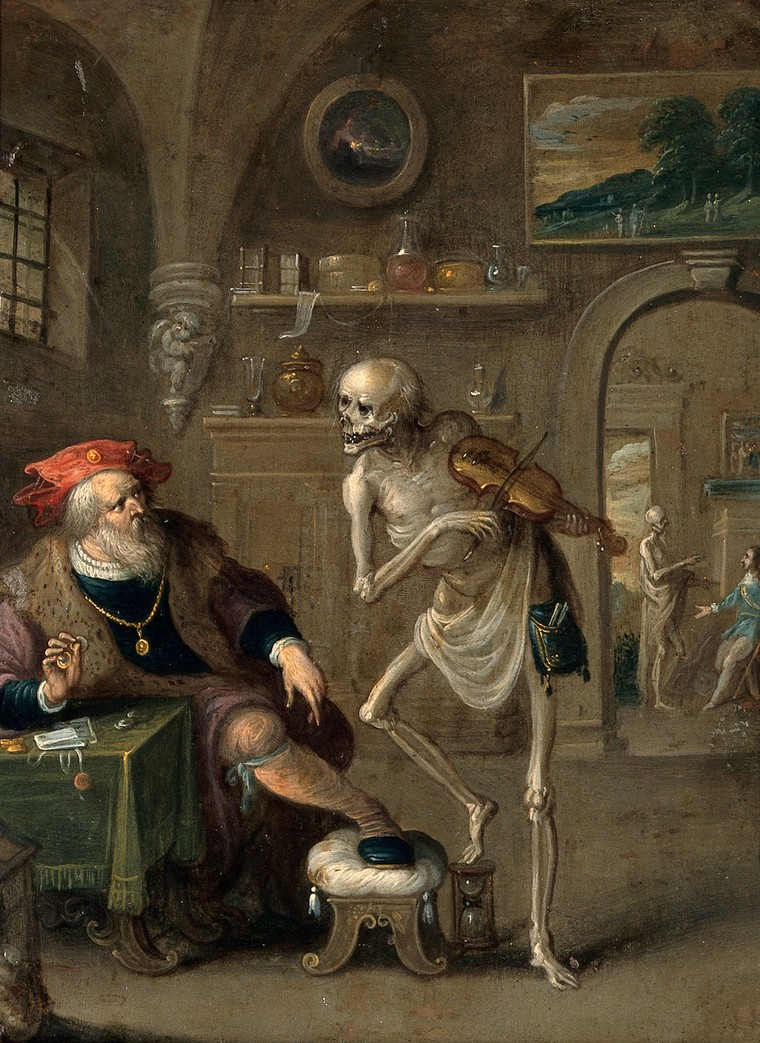
\includegraphics[height=\textwidth]{img/death_and_miser.jpg}
\captionsetup{labelformat=empty}
\caption{\small{
Франс Франкен Младший. \urlnote{Смерть и скупец}
{https://wellcomecollection.org/works/m7cumkjp/images?id=pqqx8pq7}.
XVII в. Галерея Wellcome, Лондон.
}}
\end{figure}
\setcounter{figure}{0}

\subsection{Индексное инвестирование}

Почему вообще так сложно искать <<альфу>>? Вспомните аргумент из CAPM. Что бы ни 
случилось, в совокупности все инвесторы сообща владеют одним рыночным портфелем 
на всех. Поиск <<альфы>> это игра с нулевой суммой. Чтобы кто-то имел 
положительную <<альфу>> относительно рынка, кто-то должен иметь отрицательную 
<<альфу>>. Конкуренция приводит к тому, что для получения доходности сверх той, 
что обещают модели, нужно прикладывать ощутимые усилия (ну или быть довольно 
удачливым).

Практика показывает, что управляющие фондов в среднем показывают отрицательную 
<<альфу>> с учётом комиссий. Кроме того, положительная <<альфа>> в предыдущий 
год совершенно не гарантирует положительную <<альфу>> в будущем году. Поэтому 
инвесторы зачастую получают меньшую доходность при том же уровне 
систематического риска, чем если бы они просто купили на все деньги рыночный 
портфель.

На этом наблюдении основана идея \ruen{индексного инвестирования}{index 
investing}. Пионер индустрии \ruen{Джон Богл}{John Bogle} придумал специальный 
тип паевого фонда --- индексный фонд. Управляющий индексным фондом открыто 
декларирует, что не собирается заниматься фундаментальным анализом акций 
множества компаний, чтобы выбрать самые перспективные. Вместо этого он берёт 
деньги вкладчиков и покупает все акции из индекса в той же пропорции, в которой 
они входят в индекс.

Как и обычные паевые фонды, индексный фонд берёт комиссию за свою услуги. 
Поскольку покупку акций из определения индекса можно хорошо автоматизировать и 
масштабировать хоть на 100 клиентов фонда, хоть на миллион, комиссия индексных 
фондов обычно на порядок-другой ниже, чем у обычных фондов с активным  
управлением. Например, самый крупный индексный фонд на индекс S\&P~500 от 
Vanguard стоит 0.04\% (четыре сотых процента) в год \cite{vanguard500}.

Задача индексного фонда --- не найти <<альфу>>, а дать инвестору возможность с 
минимальными накладными расходами купить желаемую <<бету>>, то есть взять на 
себя строго определённый систематический риск. Доходность индексного фонда --- в 
чистом виде премия за систематический риск минус комиссия управляющего. Если бы 
мы прогнали регрессию доходности индексного фонда на индекс, то получили бы 
<<альфу>> 0 и <<бету>> 1. Кто-то скажет, что это не так круто, но с точки зрения 
математики нулевая <<альфа>> точно лучше отрицательной.

С другой стороны, от инвестора требуется не найти гениального управляющего, 
который обеспечит <<альфу>>, а выбрать те факторы систематического риска, на 
которые он готов сделать ставку в надежде заработать премию за риск. Также может 
потребоваться усилие воли, чтобы усмирить гордыню и погасить в зародыше надежду 
оказаться тем-самым-крутым-парнем-с-доходностью-тыща-процентов. Покупая индекс, 
инвестор заранее подписывается на среднюю (во всех смыслах) рыночную доходность.

Судя по успеху индексных фондов, идея нашла отклик в сердцах многих инвесторов 
\cite{bogle2016index}. Есть широкая категория инвесторов (я в их числе), кто 
хотел бы вложиться в ценные бумаги, но не готов сделать поиск <<альфы>> своей 
профессией. Индексное инвестирование --- в самый раз для таких лентяев!

\subsection{Биржевые фонды}

У классических индексных фондов (как и у ПИФов вообще) есть некоторые 
особенности. Обычно вы можете купить пай фонда раз в сутки, в конце дня. В конце 
дня управляющий смотрит на цену закрытия (последнюю цену торгов на бирже) по 
каждой акции, умножает её на число акций, которыми владеет фонд, и получает 
\ruen{сумму чистых активов или СЧА}{net asset value, NAV} фонда. Дальше он делит 
СЧА на количество паёв фонда, которыми владеют существующие инвесторы фонда, и 
получает цену одного пая, которую вы должны заплатить.

Если вы хотите купить индекс акций утром и продать вечером, чтобы вопреки всей 
канве статьи попытаться спекулировать на краткосрочных колебаниях рынка, то 
обычный паевой фонд вам не подойдёт. Чтобы устранить это неудобство, финансисты 
придумали индексные фонды, паи которых обращаются на бирже --- \ruen{биржевые 
фонды}{exchange-traded funds, ETFs}.

Чтобы лучше понять механику работу ETF'ов, предлагаю создать свой собственный 
ETF на американский индекс S\&P~500. Не будем тратить время на споры о названии 
и назовём наш фонд \en{Romashka ETF}.

С одной стороны, ETF --- это паевой фонд, поэтому он подчиняется тому же 
регулированию, что и традиционные паевые фонды. С другой стороны, ETF --- это 
обычная компания, акции (то есть паи) которой обращаются на бирже, как и акции 
других компаний. Только в отличие от других компаний, ETF владеет не заводами, 
газетами и пароходами, а акциями компаний из индекса.

Возьмём наш начальный капитал, скажем, \dollars{100} миллионов, и купим на эти 
деньги акции. В полном соответствии с духом индекскного инвестирования, нам не 
нужно заниматься фундаментальным анализом и выбором перспективных акций. 
Напротив, нас ждёт монотонная механическая работа. Открываем на Википедии 
страничку со списком акций, входящих в индекс S\&P~500 и начинаем считать.

Всего в индексе 500 компаний. Рыночная капитализация всего индекса (рыночная 
цена всех акций всех компаний, входящих в индекс) --- \dollars{27.9} триллиона. 
Рыночная капитализация компании Apple (цена одной акции Apple, умноженная на 
количество акций Apple в обращении) --- \dollars{1.98} триллиона. Таким образом, 
доля Apple в индексе S\&P~500 равна $\dollars{1.98}/\dollars{27.9} \approx
7.1\%$. Следовательно, в портфель нашего Romashka ETF мы купим акций Apple на 
7.1\% нашего капитала, то есть на \dollars{7.1} миллиона.

Идём дальше. Рыночная капитализация Microsoft составляет \dollars{1.59} 
триллиона или 5.7\% от общей капитализации индекса. Поэтому мы купим акций 
Microsoft на 5.7\% нашего капитала, то есть на \dollars{5.7} миллиона. Рыночная 
капитализация Amazon \dollars{1.58} триллиона, это 5.7\% от капитализации 
индекса, и мы купим акций Amazon на 5.7\% капитала или на \dollars{5.7} 
миллиона. Думаю, алгоритм понятен, поэтому разрешите мне не перечислять 
остальные 497 акций.

В конце концов, если управляющий Romashka ETF не сойдёт с ума от скуки до того, 
как доберётся до конца списка, то наш фонд будет владеть миниатюрной версией 
<<большого>> индекса S\&P~500. Когда весь индекс будет расти на 1\%, то акции, 
которые принадлежат фонду, тоже будут расти на 1\%.

Теперь мы можем разместить паи самого Romashka ETF на бирже и обратиться к 
инвесторам: <<Господа! Если вы хотите купить индекс S\&P~500, то не мучайтесь и 
не покупайте каждую акцию по отдельности! Наш профессиональный управляющий уже 
сделал эту грязную работу за вас! Купите паи Romashka ETF и получите долю в 
портфеле, который совпадает с индексом! Сэкономьте на брокерских и биржевых 
комиссиях!>>

На идеальном рынке из мультфильма <<My Little Pony>> цена паёв нашего Romashka 
ETF всегда в точности следовала бы за ценой акций, которыми мы владеем. Если 
общая рыночная стоимость всех акций из портфеля равна \dollars{101232453.74}, то 
рыночная капитализация Romashka ETF (цена одной пая на бирже, умноженная на 
количество паёв) тоже должна быть равна \dollars{101232453.74}. К сожалению, в 
реальности так бывает не всегда, и цены паёв закрытых фондов могут сильно 
отклоняться от рыночной цены их портфеля.

Чтобы креко-накрепко связать цену пая Romashka ETF и цены акций из портфеля, нам 
нужна помощь акул капитализма. Обратимся в несколько крупных фирм с Уолл Стрит и 
предложим им стать \ruen{авторизованными участниками}{authorized participants} 
нашего фонда. Авторизованные участники получат право обменивать акции из индекса 
на вновь созданные для них паи Romashka ETF, а также право гасить паи, то есть 
приносить нам пай Romashka ETF и взамен получать часть акций из нашего портфеля.

Предположим, что после начальных инвестиций в \dollars{100} миллионов мы 
выпустили миллион паёв Romashka ETF стоимостью \dollars{100} каждый и распродали 
их на бирже. Мы можем выпустить для авторизованного участника ешё \num{10000} 
новых паёв, если он передаст нам взамен корзину из акций Apple, Microsoft, 
Amazon и других компаний из индекса в нужной нам пропорции. 7.1\% корзины должны 
составлять акции Apple, 5.7\% корзины должны составлять акции Microsoft, и так 
далее. С другой стороны, авторизованный участник имеет право предъявить к 
погашению \num{10000} паёв Romashka ETF, а взамен мы обязаны выдать ему корзину 
акций Apple, Microsoft и других компаний.

Для чего нужна эта магия? Это нужно, чтобы помочь невидимой руке рынка уравнять 
цены паёв Romashka ETF и акций из индекса.

Например, если инвесторы вдохновились идеей Romashka ETF и бросились скупать 
наши паи, то цена паёв может вырасти, даже если цена акций, которыми владеет 
фонд, не изменилась. Если так случится, то авторизованный участник купит акции 
Apple, Microsoft, Amazon и остальных компаний по отдельности, передаст их нам, 
получит взамен паи Romashka ETF и продаст их с прибылью страждущим инвесторам.

Спрос на отдельные акции со стороны авторизованного участника подтолкнёт цены 
вверх, а дополнительное предложение паёв Romashka ETF сдвинет их цену вниз. 
Авторизованный участник будет продолжать зарабатывать на ошибке рынка до тех 
пор, пока цены отдельных акций и паёв Romashka ETF не придут в равновесие. Эта 
ситуация изображена на рисунке \ref{etf_arbitrage_etf_expensive}.

\begin{figure}[h]
\centering
\begin{tikzpicture}
\draw (0, 1.3) node[minimum height=0.8cm]{Romashka ETF};
\draw[rounded corners] (-1.8, 1.7) rectangle (1.8, -2.0);
\draw (0, 0.4)  node[rectangle,rounded corners,draw,minimum width=3cm,minimum height=0.8cm]{Apple};
\draw (0, -0.5) node[rectangle,rounded corners,draw,minimum width=3cm,minimum height=0.8cm]{Microsoft};
\draw (0, -1.4) node[rectangle,rounded corners,draw,minimum width=3cm,minimum height=0.8cm]{Amazon};

\draw (5.7, -0.15) node[rectangle,rounded corners,draw,minimum width=3.4cm,minimum height=3.7cm]{\begin{tabular}{c}Автори-\\зованный\\участник\end{tabular}};

\draw[->,>=triangle 90] (1.8, 1.3) -- (4, 1.3) node[pos=0.5,anchor=south]{пай};

\draw[->,>=triangle 90] (4, -1.4) -- (1.8, -1.4) node[pos=0.5,anchor=north]{\begin{tabular}{c}
Apple \\ Microsoft \\ Amazon
\end{tabular}};

\draw[->,>=triangle 90] (7.4, 1.3) -- (9.6, 1.3) node[pos=0.5,anchor=south]{пай};

\draw[->,>=triangle 90] (9.6, -1.4) -- (7.4, -1.4) node[pos=0.5,anchor=north]{\begin{tabular}{c}
Apple \\ Microsoft \\ Amazon
\end{tabular}};

\draw (11.3, -0.15) node[rectangle,rounded corners,draw,minimum width=3.4cm,minimum height=3.7cm]{Рынок};
\end{tikzpicture}
\caption{Пай фонда стоит дороже корзины акций. Авторизованный участник покупает 
акции с рынка, меняет их на пай фонда, продаёт паb на рынке.}
\label{etf_arbitrage_etf_expensive}
\end{figure}

Если сложилась обратная ситуация, и паи Romashka ETF оказались дешевле, чем 
отдельные акции, то авторизованный участник запустит этот механизм в обратном 
направлении. Как показано на рисунке \ref{etf_arbitrage_etf_cheap}, он купит на 
рынке относительно дешёвые паи Romashka ETF, предъявит их нам, получит взамен 
акции Apple, Microsoft, Amazon и других компаний и с прибылью продаст их на 
бирже по отдельности.

\begin{figure}[h]
\centering
\begin{tikzpicture}
\draw (0, 1.3) node[minimum height=0.8cm]{Romashka ETF};
\draw[rounded corners] (-1.8, 1.7) rectangle (1.8, -2.0);
\draw (0, 0.4)  node[rectangle,rounded corners,draw,minimum width=3cm,minimum height=0.8cm]{Apple};
\draw (0, -0.5) node[rectangle,rounded corners,draw,minimum width=3cm,minimum height=0.8cm]{Microsoft};
\draw (0, -1.4) node[rectangle,rounded corners,draw,minimum width=3cm,minimum height=0.8cm]{Amazon};

\draw (5.7, -0.15) node[rectangle,rounded corners,draw,minimum width=3.4cm,minimum height=3.7cm]{\begin{tabular}{c}Автори-\\зованный\\участник\end{tabular}};

\draw[<-,>=triangle 90] (1.8, 1.3) -- (4, 1.3) node[pos=0.5,anchor=south]{пай};

\draw[<-,>=triangle 90] (4, -1.4) -- (1.8, -1.4) node[pos=0.5,anchor=north]{\begin{tabular}{c}
Apple \\ Microsoft \\ Amazon
\end{tabular}};

\draw[<-,>=triangle 90] (7.4, 1.3) -- (9.6, 1.3) node[pos=0.5,anchor=south]{пай};

\draw[<-,>=triangle 90] (9.6, -1.4) -- (7.4, -1.4) node[pos=0.5,anchor=north]{\begin{tabular}{c}
Apple \\ Microsoft \\ Amazon
\end{tabular}};

\draw (11.3, -0.15) node[rectangle,rounded corners,draw,minimum width=3.4cm,minimum height=3.7cm]{Рынок};
\end{tikzpicture}
\caption{Пай фонда стоит дешевле корзины акций. Авторизованный участник покупает 
паи фонда с рынка, меняет их на акции, продаёт акции на рынке.}
\label{etf_arbitrage_etf_cheap}
\end{figure}

Как видите, механизм авторизованных участников может сделать так, что паи 
Romashka ETF всегда будут повторять динамику индекса S\&P~500. Лично мне больше 
всего нравится то, что механизм работает не за счёт каких-то там джентльменских 
договорённостей, а за счёт вполне конкретных материальных стимулов. 
Авторизованный участник зарабатывает деньги ровно за то, что устраняет разницу в 
ценах фонда и акций. Поэтому он кровно заинтересован в том, чтобы делать это как 
можно лучше и как можно быстрее, пока ошибку рынка не исправили конкуренты.

\subsection{Риски биржевых фондов}

В целом я считаю биржевые фонды отличной финансовой инновацией. Однако, было бы 
нечестно не рассказать вам о рисках, специфичных для этого способа инвестиций. Я 
не думаю, что эти риски достаточно высоки, чтобы отказаться от биржевых фондов, 
но знать о них нужно.

Во-первых, механизм авторизованных участников может дать сбой в кризис. Я имею 
удовольствие владеть ETF'ом на облигации, который в марте этого года временно 
просел на 6\% относительно справедливой рыночной цены бумаг, составляющих фонд. 
Надо полагать, в кризис рынок стал менее ликвидным, и авторизованные участники 
не могли совершить арбитражную сделку по покупке паёв ETF'а, обмена их на 
отдельные облигации и продаже облигаций на рынке.

Конечно, в течение нескольких недель всё нормализовалось, и цены паёв фонда 
выросли и сравнялись с ценой отдельных облигаций. Тем не менее, я до сих пор 
помню, насколько я был ошарашен, ошеломлён и обескуражен, когда фонд надёжных 
облигаций в моём портфеле упал на 6\%. Если бы именно в тот момент мне срочно 
понадобились деньги и пришлось бы продавать паи фонда по рыночной цене, то было 
бы очень обидно.

Во-вторых, некоторые фонды зарабатывают деньги на том, что иногда дают свои 
ценные бумаги \ruen{в долг}{margin lending}. Как я уже упоминал, иногда у 
инвесторов возникает желание продать акцию, которой у них нет, чтобы заработать 
на снижении цены. Почти как мечтали герои <<Простоквашино>>: продать что-то 
ненужное подороже, а потом купить его же подешевле. Чтобы это сделать, инвестор 
должен у кого-то одолжить акцию.

Попросить акцию в долг у индексного фонда --- отличная идея, потому что у фонда 
огромный портфель с сотнями, если не тысячами, акций, среди которых наверняка 
есть нужная. Инвестор одалживает у фонда акцию, а взамен даёт живые деньги в 
качестве залога. Обычно залог составляет 105\%--110\% от рыночной цены бумаги. 
Если вдруг инвестор не вернёт акцию в срок, то фонд заберёт себе залог и сам 
купит акцию на рынке, чтобы клиенты фонда не пострадали. Запас в 5\%--10\% 
защищает фонд от неожиданного роста цены акции.

Для чего это фонду, спросите вы? Дело в том, что он имеет право положить на 
депозит деньги, которые получил в залог, и заработать проценты. Это довольно 
выгодно, потому что акция ценой \dollars{100} не зарабатывает проценты, а вот 
полученные за неё \dollars{105} --- да. Учитывая, что комиссия фондов может 
составлять сотые процента в год, дополнительная прибыль от предоставления акций 
в долг может быть очень кстати.

Так вот, гипотетически возможен сценарий, когда фонд отдаст в долг слишком много 
акций, а их не вернут. Если так сложится, что одновременно цена акций вырастет, 
то фонду не хватит залога, чтобы выкупить акции с рынка. В результате в фонде 
останется меньше акций, чем было, и владельцы паёв фонда понесут убытки.

Насколько я понимаю, законодательство запрещает фондам давать в долг больше, 
чем треть акций \cite{wsj2011lending}. Кроме того, даже этот лимит фонды не 
используют. Например, в моём портфеле есть фонд iShares S\&P~500. Согласно 
годовому отчёту \cite{ishares2020report}, при суммарной стоимости всех акций в 
фонде \dollars{161} миллиард фонд выдал в долг акций на \dollars{3.3} миллиарда, 
то есть чуть больше 2\% всех активов фонда. Поэтому я (пока?) не очень опасаюсь 
этого риска.

Третий вид риска, о котором стоит знать, относится к так называемым 
\ruen{синтетическим}{synthetic} фондам. Иногда управляющая компания фонда 
считает, что купить корзину активов может быть слишком сложно из-за высоких 
накладных расходов. Тогда она покупает у крупного банка специальный дериватив, 
\ruen{своп полного дохода}{total return swap}. Банк обязуется в будущем 
выплатить фонду ровно те же деньги, которые получил бы реальный владелец актива. 
Особенно часто такая структура встречается среди фондов на биржевые товары и 
ценные металлы, в том числе золото.

Само по себе это не криминал, но нужно понимать, что у держателей паёв фонда 
появляется небольшой кредитный риск на банк. Конечно, дериватив тоже обеспечен 
залогом, но всё равно можно представить ситуацию, когда банк не сможет выполнить 
свои обязательства перед фондом, а залога не хватит, чтобы покрыть убыток.

Наконец, четвёртый риск, о котором я хотел рассказать, важен скорее регуляторам, 
чем частным инвесторам. Есть опасение, что биржевые фонды могут сыграть 
негативную роль в кризис, потому что они упрощают инвесторам как вход на рынок 
(купить пай проще, чем 500 акций из индекса), так и выход.

Если все инвесторы ETF'ов встанут не с той ноги и решат продать свои паи, то 
упадут и все акции, входящие в индекс, потому что авторизованные участники чисто 
механически начнут продавать отдельные акции. Это может вызвать волну распродаж 
на рынке акций, которая подстегнёт новые продажи со стороны индексных 
инвесторов. В общем, получится замкнутый круг и классическая биржевая паника. 
Подробнее об этом механизме можно прочитать в отчёте \cite{pagano2019can}.

Возможно, стоило бы упомянуть про риск того, что управляющий фонда сложит акции 
в мешок, спустится из окна по верёвке и скроется в неизвестном направлении. 
Честно говоря, я пока не слышал о таких случаях. В Европе и в США биржевые фонды 
подчиняются тому же законодательству, что и паевые фонды, поэтому интересы 
инвесторов защищены. 

Если вы опасаетесь этого риска, то решение должно быть не в том, чтобы  
отказаться от биржевых фондов вообще, а в том, чтобы вспомнить главное идею этой 
статьи --- диверсификацию. Купите несколько фондов разных управляющих компаний, 
и тогда риск случайного банкротства одной из них будет не так страшен.

\subsection{Технический анализ}

Всё это индексное инвестирование выглядит как-то скучно, не правда ли? Купите
индекс, подождите 20 лет, продайте индекс. В рекламе биржевая торговля выглядит
совсем не так. Молодой человек или девушка пристально вглядывается в 
разноцветные графики на огромных мониторах. Крупный план: зрачки сужаются, на 
графиках видна аномалия. Несколько секунд напряжённых размышлений, пара кликов 
мышкой --- и вот на счету прибавляется пара тысяч долларов. Заработать на 
бирже просто!

Действительно, на бирже можно заработать <<просто>>, если взять на себя 
систематический риск и на дистанции нескольких лет заработать премию за этот 
риск. А вот к идее пристального разглядывания графиков и к краткосрочным 
спекуляциям в течение дня я отношусь крайне скептически.

Существуют ли люди, которые заработали деньги краткосрочными спекуляциями на 
рынке акций или на валютном рынке? Да, разумеется. Чего больше в их успехе --- 
удачи или умения? Сами трейдеры, конечно, объяснят свой успех упорной работой и 
бессонными ночами за учебниками. Я склонен видеть здесь больше удачи, хотя 
кто-то назовёт мою реакцию завистью.

Представим, что вы пришли в казино играть в рулетку. На рулетке 18 красных 
секторов, 18 чёрных и 1 сектор зеро. Есть ли у вас шанс увеличить свою ставку в
2 раза, угадав красное или чёрное? Конечно! Шанс угадать и удвоиться равен 
$18/37$ или $48.6\%$. Скажу даже больше, у вас есть ненулевой шанс увеличить 
свой капитал в 1024 ($2^{10}$) раза. Нужно всего-навсего 10 раз подряд угадать 
красное или чёрное. Вероятность угадать составляет $(18/37)^{10}$ или 0.074\%, 
то есть один шанс из 1347.

Вы считаете, что 1 шанс из 1347 это немного? Как посмотреть. Если в казино 
придут \num{100000} человек, то в среднем $\num{100000}/1347 = 74$ из них 
угадают красное или чёрное 10 раз подряд и увеличат свой капитал в \num{1024} 
раза. Остальные \num{99926} посетителей покинут казино с пустыми карманами, но 
кого это волнует? Зато эти 74 счастливчика смогут сниматься в рекламе, писать 
мотивирующие статьи и читать лекции о том, как выигрывать в рулетку.

В чём вообще проблема с техническим анализом, то есть разглядыванием графиков
цен и поиском закономерностей? Дело в том, что он противоречит представлениям
экономистов о том, как функционирует рынок \cite[ch.~11.2]
{bodie2014investments}. Изменение цен активов слишком близко к \ruen{случайному 
блужданию}{random walk}, чтобы изучение графиков и поиск повторяющихся шаблонов 
имело какой-то смысл.

\subsection{Эффективность рынка}

Согласно \ruen{гипотезе эффективного рынка}{efficient market hypothesis}, 
рыночная цена акций и других активов отражает всю известную информацию. Если 
эта гипотеза верна, то вы не сможете заработать деньги, просто глядя на графики 
цен, потому что эта информация уже и так известна всем. Так что можете выкинуть 
учебник по техническому анализу. Изучение отчётности компаний (так называемый 
фундаментальный анализ) тоже под вопросом, потому что данные из отчётности 
публичны и доступны всем участникам рынка \cite[ch.~11]
{bodie2014investments}.

Конечно, гипотеза эффективного рынка --- это теоретическая концепция. Насколько
хорошо она описывает реальность? Как быстро вновь поступающая информация
оказывается учтённой в цене акций? Чтобы вы прониклись тем, насколько 
эффективным может быть рынок, расскажу вам такую историю.

28-го января 1986-го года через минуту после запуска потерпел крушение 
космический челнок <<Челленджер>>. Погибли все 7 членов экипажа (первый случай 
гибели американских астронавтов во время космического полёта). Правительство 
сформировало комиссию по расследованию причин катастрофы, в которую в том числе 
вошли Ричард Фейнман и Нил Армстронг. Невидимая рука рынка также засучила 
рукава (рукав?) и принялась за работу. 

В постройке <<Челленджера>> принимали участие четыре крупных подрядчика, акции 
которых торговались на бирже. Это Lockheed, Martin Marietta, Morton Tiokhol и 
Rockwell. В течение нескольких минут после катастрофы акции всех четырёх 
компаний упали, видимо, из-за неуверенности инвесторов в будущем программы 
космических челноков.

Впрочем, в концу дня акции трёх из четырёх подрядчиков отыграли падение, и 
только акции Morton Tiokhol закончили день падением на $12\%$ и потеряли 
\dollars{200} миллионов капитализации. В следующие несколько месяцев акции 
Lockheed, Martin Marietta и Rockwell росли вместе с индексом Dow Jones, а акции 
Morton Tiokhol так и топтались на месте.

9 июня 1986-го года комиссия представила свой отчёт президенту Рейгану. 
Катастрофа случилась из-за дефекта уплотнительных колец в боковом 
твердотопливном ускорителе. Горячие газы, выходящие из ускорителя, прожгли 
оболочку центрального топливного бака и вызвали взрыв.

Как вы думаете, кто из подрядчиков отвечал за производство дефектного 
твердотопливного ускорителя? Вы правы, это была Morton Tiokhol. Штрафы, 
компенсации семьям погибших и упущенная прибыль от отменённых заказов обошлись 
компании примерно в \dollars{200} миллионов \cite{maloney2003complexity}. 
Фондовый рынок верно определил виновного и оценил его убытки за считанные минуты 
после катастрофы. Напоминаю, что это 1986-й год, до изобретения интернета и 
трансляций в разрешении HD на Ютубе.

Можно ли заработать на рынке деньги, если иметь преимущество в информации? Да,
безусловно. Может ли частный инвестор иметь преимущество в информированности 
перед теми, для кого сбор информации --- постоянная работа на полный рабочий 
день? Весьма сомнительно. Каждый раз, когда вам кажется, что вот сейчас-то рынок
точно ошибается, а вы правы, вспомните о <<Челленджере>> и перепроверьте (как 
говорят у нас на работе, почелленджите) свои аргументы ещё раз.

\subsection{Эффективно неэффективные рынки}

Если перестать травить байки и говорить серьёзно, то является ли реальный рынок 
идеально эффективным рынком из экономической теории? Если да, то все инвесторы 
должны вкладываться в дешёвые индексные фонды и отказаться от поиска <<альфы>>. 
Нет никакого смысла искать новую информацию, если цены акций уже учитывают эту 
информацию, и на ней нельзя заработать. 

Икорный социалист внутри меня был бы рад запретить все фонды, кроме индексных, 
а всех этих управляющих-спекулянтов направить работать управдомами, но всё не 
так просто.

Рынок не становится эффективным сам по себе. Эффективным его делают 
инвесторы, которые постоянно ищут новую информацию и высматривают те цены, 
которые не успели под неё подстроиться. Когда такой инвестор покупает ошибочно 
недооценённую акцию, то увеличение спроса толкает цену вверх, ближе к 
фундаментально обоснованному значению. Если все будут инвестировать только в 
индексные фонды, то кто же будет следить за эффективностью рынка?

В равновесии, на рынке должно быть достаточно \ruen{неэффективностей}
{ineffeciences}, чтобы компенсировать инвестору расходы на поиск информации и 
риск, который он несёт, пока исправляет ошибку рынка. С другой стороны, 
неэффективностей должно быть не слишком много, чтобы потенциальные новые игроки 
не видели выгоды в приходе на этот сегмент рынка. Автор книги
\cite{pedersen2015efficiently} называет это <<эффективной неэффективностью>>. 
Короче говоря, можно заработать на ошибках рынка, но это совсем не просто, и в 
этой области своя конкуренция.

Есть ещё одна полезная функция, помимо поиска новой информации, которая 
вознаграждается рынком --- предоставление ликвидности. Часто на рынке есть 
участники, которые по той или иной причине готовы заключить сделку по цене, 
которая чуть отличается от фундаментально обоснованной, если сделку можно будет 
заключить здесь и сейчас.

Например, пенсионный фонд может продавать облигацию, потому что её кредитный 
рейтинг упал ниже BBB, и теперь законодательство запрещает держать её в 
портфеле. Или индексный фонд может продавать акцию, которая выпала из индекса и 
теперь только мешает фонду следовать за индексом. В обоих случаях участники 
рынка действуют не исходя из фундаментальной оценки активов, а под влиянием 
внешних нерыночных факторов.

Факторы, которые ограничивают участников рынка в выборе, называются 
\ruen{рыночными трениями}{market frictions}. Если управляющий фондом будет 
помогать остальным преодолевать эти трения, предоставляя ликвидность, то он
может получить (или не получить) награду за свою услугу. Дальше я приведу 
один интересный пример рыночного трения и того, как на нём можно заработать.

Как вы помните, одно из предположений CAPM состоит в том, что инвесторы могут 
занимать деньги под безрисковую процентную ставку. Что, если это не так? В 
реальной жизни многим игрокам, таким как паевые фонды для розничных клиентов, 
запрещено использовать заёмные деньги. Другие инвесторы могут сознательно 
ограничить себя в использовании заёмных средств (торговли <<с плечом>>), 
опасаясь связанных с ним рисков.

На рисунке \ref{efficient_frontier_with_risk_free_no_leverage} изображена 
граница эффективности, с которой столкнутся инвесторы, которые не могут 
использовать заёмные средства. Слева от касательного рыночного портфеля T мы
видим привычную прямую линию из CAPM. Справа от касательного портфеля T граница
эффективности повторяет кривую линию --- границу эффективности для портфелей, 
составленных из рискованных активов.

\begin{figure}[h]
\centering
\begin{tikzpicture}
\begin{axis}[
    width=\textwidth,
    xlabel={Стандартное отклонение, \%},
    ylabel={Ожидаемая доходность, \%},
    xmin=0, xmax=14,
    ymin=0, ymax=10
]

    \newcommand{\drawAssetNode}[4]{
        \node[
            circle,
            fill,
            inner sep=2pt
        ]
        at (axis cs: #1, #2)
        {};
        
        \node[
            anchor=#4
        ]
        at (axis cs: #1, #2)
        {\small #3};
    }

    \newcommand{\drawPortfolioNode}[8]{
        \node[
            anchor=#8
        ]
        at (axis cs: #1, #2) {
            \small
            \begin{tabular}{|l|r|}
                \hline
                \multicolumn{2}{|c|}{#3} \\ \hline
                Акц. & #4\% \\
                Обл. & #5\% \\
                Нед. & #6\%  \\
                Зол. & #7\% \\
		          \hline
           \end{tabular}
        };
	
        \node[
            circle,
            fill,
            inner sep=3pt,
            color=Set1-B
        ]
        at (axis cs:#1, #2)
        {};
    }

    \newcommand{\drawPortfolioNodeTwo}[6]{
        \node[
            anchor=#6
        ]
        at (axis cs: #1, #2) {
            \small 
            \begin{tabular}{|l|r|}
                \hline
                \multicolumn{2}{|c|}{#3} \\ \hline
                Портф. T & #4\% \\
                Безриск. & #5\% \\
                \hline
            \end{tabular}
        };

        \node[
            circle,
            fill,
            inner sep=3pt,
            color=Set1-B
        ] at (axis cs:#1, #2)
        {};
    }

    \newcommand{\drawCapmLine}[2] {
        \addplot[
            line width=1pt,
            color=Set1-B, 
            domain=#1,
            #2
        ]
        {4 + x * (6.75 - 4) / 4.83};
    }

    \newcommand{\drawRiskyFrontier}[2] {
        \addplot[
            line width=1pt,
            color=Set1-B,
            restrict x to domain=#1,
            #2
        ]
        table[
            x=std_dev,
            y=target_return,
            col sep=comma
        ]
        {data/efficient_frontier_plot_data.csv};
    }

    \drawCapmLine{0:4.83}{solid}

    \drawCapmLine{4.83:21}{dashed}

	 \drawRiskyFrontier{0:4.83}{dashed}
	 
	 \drawRiskyFrontier{4.83:21}{solid}

    \drawPortfolioNodeTwo{1.45}{4.83}{Портфель А}{30}{70}{north west}

    \drawPortfolioNodeTwo{4.83}{6.75}{Портфель B}{100}{0}{north west}

    \drawPortfolioNodeTwo{7.25}{8.12}{Портфель C}{150}{-50}{north west}

    \drawAssetNode{0.0}{4.0}{}{west}

    \drawPortfolioNode{4.83}{6.75}{Портфель T}{24.2}{69.5}{1.5}{4.8}{south east}

\end{axis}
\end{tikzpicture}

\caption{Граница эффективности для портфелей, составленных из акций, облигаций,
недвижимости, золота и безрискового актива, если инвесторы не могут занимать 
деньги под безрисковую ставку.}
\label{efficient_frontier_with_risk_free_no_leverage}
\end{figure}

Портфель C, состоящий на -50\% из безрискового актива (заёмных средств) и 150\% 
касательного портфеля T, больше не доступен инвестору, который не может брать 
деньги в долг. Если инвестора не устраивает доходность 6.75\%, которую ему 
обещает касательный портфель, то более доходный и рискованный портфель он может 
составить только из доступных ему  рискованных активов, в основном акций и 
фондов недвижимости.

На рынке возникает дополнительный спрос на более рискованные активы, которые 
дают более высокую доходность, чем касательный портфель. Такими активами могут
быть, например, акции с <<бетой>> больше 1, которые в хорошие времена растут
быстрее рынка. Но если спрос на такие акции повышается, то невидима рука рынка
увеличивает их цену и снижает ожидаемую доходность.

С другой стороны, инвесторы, которые не берут деньги в долг, но ищут 
доходность, не обращают внимание на активы с доходностью и риском меньше, чем у 
рыночного портфеля. Например, акции с <<бетой>> меньше 1 пользуются меньшим 
спросом, поэтому их цена становится ниже, а ожидаемая доходность --- выше.

Можно составить синтетический портфель, который будет покупать акции с низкой 
<<бетой>> и продавать акции с высокой <<бетой>>. Авторы называют этот портфель
\ruen{<<ставь против беты>>}{bet against beta, BAB}. Оказывается, что на 
длинной дистанции этот портфель зарабатывал 8.4\% в год (сравнимо с индексом 
акций) при волатильности 11\% (почти в два раза ниже рынка акций)
\cite{frazzini2014betting}.

Управляющий или частный инвестор, который не имеет ограничений в использовании 
заёмных средств, может заработать прибыль, если будет покупать акции с низкой 
<<бетой>> и продавать в короткую акции с высокой <<бетой>>. Можно считать, что 
такая прибыль --- это награда за полезную работу по удовлетворению повышенного 
спроса на акции с высокой <<бетой>>. Если бы управляющий не занимался 
предоставлением ликвидности, то \sout{её предоставляли бы солдаты НАТО} 
остальные инвесторы покупали бы акции с высокой <<бетой>> по более высокой цене 
и зарабатывали бы меньшую ожидаемую доходность.

Надо сказать, что портфель BAB, как и остальные факторные портфели, это вовсе 
не станок для печатания денег. Фонд, который занимает деньги, чтобы составить 
портфель BAB, может в какой-то момент столкнуться с трудностями при привлечении
средств. Стратегия BAB имеет свойство разваливаться, когда рынок кредитования
переживает кризис и процентные ставки резко растут. Так что избыточная 
доходность портфеля BAB --- это тоже премия за систематический риск.

На мой взгляд, фактор BAB --- отличный пример того, как можно заработать деньги 
на рынке. Если на вас не распространяются те же регуляторные ограничения, что и
на остальных участников, или если у вас другой профиль чувствительности к
риску, или же если у вас есть технологическое преимущество, то вы в самом деле 
можете заработать на трениях и неэффективностях рынка. Однако, для этого вам
придётся взять на себя риск, который не могут или не хотят брать остальные, и 
ваша прибыль будет ничем иным как премией за этот риск.

\subsection{Лирическое отступление о пользе моделей}

По мере того, как мы приближаемся к концу статьи, вас наверняка гложет вопрос: 
а насколько вообще релевантны CAPM и другие модели, о которых я рассказал вам?

Если бы CAPM выполнялась на 100\%, то, во-первых, финансы были бы очень скучной
наукой, а во-вторых, не было бы нужды придумывать APT и факторные модели. Сам 
факт того, что для объяснения доходностей активов и портфелей нам нужны все эти 
SMB, SOE и BAB, говорит, что доходности активов в реальном мире не всегда точно 
совпадают с предсказаниями CAPM.

Нужно понимать, что CAPM --- это прежде всего модель, которая в первом 
приближении описывает реальность, но совершенно не претендует на роль 
финансовой <<теории всего>>. Даже беглый взгляд на предположения CAPM говорит, 
что вряд ли можно ожидать 100\% совпадения с реальностью
\cite[ch.~14.2]{welch}.

Сложно поверить, что все инвесторы на рынке это рациональные роботы, которые 
наперёд знают будущие распределения доходностей активов вместе со всеми 
ковариациями между ними. Кроме того, CAPM не видит многие активы, которые
не торгуются на фондовом рынке, но для многих людей составляют значительную 
часть богатства. Это личная недвижимость и человеческий капитал (возможность 
работать и получать зарплату в будущем).

Похожая ситуация с портфельной оптимизацией, о которой я рассказал вам в первой 
части. Мы предположили, что доходность измеряется мат. ожиданием, а риск --- 
дисперсией. Однако, если спросить случайного человека с улицы, он скажет, что 
дисперсия <<вверх>> (неожиданно большой доход) пугает не так, как дисперсия 
<<вниз>> (неожиданно низкий доход). Дисперсия --- это лишь приближение того, 
как люди воспринимают риск. Можно сформулировать альтернативные задачи 
оптимизации, в которых риск будет измеряться, скажем, средними потерями в 
худшем 1\% случаев \cite{krokhmal2002portfolio}.

Означает ли это что CAPM и портфельную оптимизацию нужно сдать в утиль? Скорее 
нет, чем да. Никто же не сдаёт в утиль Ньютоновскую физику. Даже чисто с точки
зрения педагогики, эти теории дают полезное понимание базовых идей. Польза 
диверсификации, соотношение идиосинкратического и систематического риска, 
премия за риск --- все эти понятия оживают в математических моделях.

Мы можем спорить о том, нужно ли добавлять в задачу оптимизации дисперсию или 
другую меру риска, или является ли факторный портфель SMB (маленькие компании 
против больших) статистически значимым фактором систематического риска. Но сам 
этот спор возможен благодаря тому, что у нас есть модели. Никакая модель (в 
любой науке, не только в экономике) не описывает всю наблюдаемую Вселенную, но 
это не мешает использовать модели, чтобы лучше понимать причинно-следственные 
связи.

Даже если вы нашли свой собственный уникальный способ заработать на рынке без
риска, то всё равно имеет смысл сделать паузу и посмотреть, что об этом думает
наука. Возможно, вы взяли на себя дополнительный систематический риск, как в
случае с фактором SOE (частные компании минус государственные) в портфеле 
автора. Возможно, вы наткнулись на неэффективность рынка или рыночные трения, 
которые не совпадают с предположениями моделей, как в случае со стратегией 
<<ставь против беты>>. Перефразируя классика, модель --- ложь, да в ней намёк, 
добрым молодцам урок.

\subsection{Личный опыт и сбережения на пенсию}

Учитывая фиаско с нулевой <<альфой>>, совершенно не очевидно, почему вы должны
прислушиваться к моему мнению об инвестициях. Я привожу этот раздел не столько
для того, чтобы дать вам совет, сколько для того, чтобы продемонстрировать, что
мои слова не расходятся с делом, когда речь заходит о собственной шкуре.

В таблице \ref{personal_portfolios} представлены все наши с супругой инвестиции
в ценные бумаги по состоянию на октябрь 2020-го года. Как видите, я стараюсь
следовать своим же советам. Когда это возможно, я инвестирую в индексные фонды 
с низкими комиссиями за управление. При этом я диверсифицируюсь как по типам
ценных бумаг (есть и акции, и облигации), так и по регионам и валютам (есть и
американские, и европейские, и российские бумаги), и по управляющим компаниям 
фондов.

\begin{table}[h]
\centering
\begin{tabular}{l|l|l}
Портфель        & Регион & Инструменты \\
\hline
Сам себе пенсия & Мир    & Vanguard VT (индекс акций FTSE Global), \\
                &        & FinEx FXUS (индекс акций MSCI USA), \\ 
                &        & FinEx FXCN (индекс акций MSCI China), \\
                &        & FinEx FXDE (индекс акций MSCI Germany) \\
\hline
Сам себе ETF    & Россия & <<Акрон>>, <<Аэрофлот>>, <<Лукойл>>, \\
                &        & <<МосБиржа>>, <<МТС>>, <<Норникель>>,\\
                &        & <<Татнефть-п>>, <<Черкизово>>, <<Юнипро>>, \\
                &        & инфляционные облигации ОФЗ-ИН 52001 \\
\hline
Отток капитала  & США    & iShares IVV (индекс акций S\&P~500), \\
                &        & iShares IGSB (индекс корп. облигаций) \\
\cline{2-3}
                & Европа & Xtrackers DX2X (индекс акций STOXX 600), \\
                &        & Xtrackers D5BG (индекс корп. облигаций)
\end{tabular}
\caption{Личные инвестиции автора статьи.}
\label{personal_portfolios}
\end{table}

Общее соотношение акций к облигациям и депозитам получается примерно 35/65 с 
учётом <<пенсионного>> портфеля, или 15/85 без него. Как видите, я довольно 
пугливый инвестор, что, видимо, связано с чертами характера. В разрезе валют 
выходит треть инвестиций в долларах (в долларовых акциях и облигациях), треть в 
евро, треть в рублях. Такая композиция портфеля отвечает главному требованию. С 
ней я спокойно сплю по ночам, даже когда курсы валют сходят с ума, а рынок 
акций падает на треть из-за пандемии.

Отдельно хочу рассказать про <<пенсионный>> портфель. Я убеждён, что если не 
случится чуда в виде структурных реформ и внезапного экономического роста, то 
государство не сможет обеспечить достойную пенсию ни мне, ни моим ровесникам. 
Единственный выход, который я вижу --- копить на пенсию самостоятельно сверх 
тех обязательных платежей в пенсионный фонд, которые взимает государство.

Мы с женой договорились о простом механическом правиле. Каждый раз, когда на 
карточку падает зарплата, 10\% суммы автоматически уходит на специальный 
брокерский счёт. На эти деньги я раз в месяц покупаю ETF'ы на иностранные акции 
на Московской бирже, после чего забываю о них на ближайшие 30 лет. Остановимся 
подробнее на том, почему я поступаю именно так.
 
Почему именно акции? Я думаю, что на горизонте нескольких десятков лет акции 
обеспечат лучшее сочетание риска и доходности. Вспомните график рыночной премии 
за риск \ref{us_market_premium_figure} и раздел о близоруком избегании риска. 
Наверняка мы увидим ещё не один обвал рынка, но на дистанции рынок акций будет 
расти. А если нет, то в 2051\nobreakdash-м году 65\nobreakdash-летний автор 
будет очень зол на 29\nobreakdash-летнего автора образца 2015\nobreakdash-го 
года, придумавшего этот хитрый план, но уже ничего не сможет ему сделать. 
Ошибки молодости, что поделать.

Почему именно иностранные акции? Снова диверсификация. Если вкладываться в 
российские активы, то и пенсия от государства, и доходность личных сбережений 
будут тесно связаны с российской экономикой. Будут структурные реформы и 
экономический бум --- будут и высокая государственная пенсия, и хорошая отдача 
от личных накоплений. Будет стагнация и нефть по \dollars{20} --- останусь и без 
пенсии, и без накоплений. Инвестиции в иностранные бумаги уменьшают корреляцию 
благосостояния на старости с самочувствием российской экономики.

Почему именно ETF'ы? Я не тешу себя надеждами, что смогу выбрать перспективные 
акции на американском или европейском рынке лучше, чем профессионалы, которые 
занимаются этим по 8 часов 5 дней в неделю и всё равно имеют <<альфу>> около 
нуля. Чтобы генерировать <<альфу>>, нужно жить и дышать этим рынком, а у меня и 
так есть работа мечты на 40 часов в неделю в лучшем инвестбанке Европы. Если 
нет никаких шансов обогнать индекс на дистанции 30 лет, разумно инвестировать в 
этот самый индекс.

В моём хитром плане есть одна загвоздка. ETF'ы, которые можно купить на 
российском рынке, имеют относительно высокую комиссию за управление, порядка 
0.5\%--1.0\% в год. Это едва ли не на порядок выше комиссий иностранных ETF'ов. 
В случае инвестиций на 30 лет такие комиссии могут съесть значительную часть 
накоплений и ухудшить результат. Поэтому я предпочитаю переводить накопления на 
пенсию в более дешёвый ETF Vanguard VT, который состоит из примерно 8800 акций 
со всей планеты и стоит 0.08\% в год.

Чтобы покупать ETF'ы, которые торгуются на иностранных биржах, вам нужно будет 
открыть специальный счёт либо у российского брокера (скорее всего, потребуется 
статус квалифицированного инвестора), либо у иностранного. Я не буду давать 
конкретных названий, но есть брокеры в США и в Европе, которые могут удалённо 
открыть счёт гражданам России. Для сумм от \dollars{10 000} это вполне имеет 
смысл. Кстати, как вы можете догадаться, в рамках диверсификации я открыл счета 
и у российского брокера, и у американского, и у европейского.

К сожалению, накладные расходы на конвертацию рублей в доллары и перевод 
долларов на брокерский счёт могут оказаться неподъёмными. Например, если SWIFT-
перевод стоит минимум \dollars{25} независимо от суммы, то при переводе 
\dollars{1000} вы заплатите целых 2.5\%, что съест всю экономию на комиссиях 
ETF'ов за несколько лет. Не знаю, как у вас, а у меня не такая высокая зарплата, 
чтобы 10\% от неё составляли хотя бы \dollars{1000}, поэтому в процентном 
отношении я бы платил ещё больше.

Поэтому я решил, что лучше раз в месяц покупать за рубли ETF'ы на Московской 
бирже. Раз в год я продаю накопления за год, перевожу всю сумму в доллары и 
покупаю на них иностранный ETF. За год набегает приличная сумма (12 раз по 10\% 
это больше месячной зарплаты), так что фиксированные накладные расходы 
составляют уже не 2.5\% от суммы инвестиций, а на порядок меньше. Надеюсь, что 
со временем конкуренция снизит комиссии российских ETF'ов, и можно будет не 
заниматься этой эквилибристикой.

Теперь вы знаете, как я инвестирую свои деньги и коплю на пенсию. Универсальных 
решений нет, и то, что подходит мне, не обязательно подойдёт вам. Кто знает, 
что бы я писал (и писал ли вообще), если бы начал инвестировать не в растущий 
рынок 2015-го, а в стагнирующий рынок 2007-го.

Я призываю вас хотя бы задуматься о накоплениях на старость. Согласно известной 
пословице, лучший момент посадить дерево был 20 лет назад, а второй лучший 
момент --- сейчас. Посадите дерево!

\clearpage
\sectionWithToc{Заключение}

Если я могу дать вам один совет по итогам всей статьи, то он будет состоять из 
одного слова. Диверсифицируйтесь! Инвестируйте в разные классы активов 
(например, акции и облигации), в разные активы внутри каждого класса, в разных
валютах и в разных странах, через разных брокеров, держите деньги в разных 
банках. Диверсификация --- единственный бесплатный обед на рынке.

Всегда оценивайте, какой риск вы (или ваш управляющий) взяли на себя. Помните, 
что далеко не каждый риск вознаграждается рынком. Покупаете ценную бумагу, 
потому что она недооценена? Подумайте, какой информацией может обладать 
продавец, почему вы готовы брать на себя риск этой бумаги, а он --- нет.

Если вы не готовы сделать поиск <<альфы>> своей профессией и посвящать этому
значительное время, то рассмотрите опцию индексных инвестиций. Индексный ПИФ 
или ETF с низкой комиссией за управление позволит вам купить именно ту <<бету>> 
(тот систематический риск), которую вы хотите, и заработать премию за риск. 
Нулевая <<альфа>> к индексу чисто математически лучше, чем отрицательная.

Соизмеряйте рискованность инвестиций с горизонтом планирования. Акции хороши на 
долгом горизонте, но совершенно не подходят для инвестиций на полгода. Если вы 
делаете долгосрочные инвестиции, то не проверяйте состояние счёта каждый день. 
Если возможно, не инвестируйте все деньги разом, а разбейте сумму на несколько 
частей, чтобы снизить вероятность просидеть без доходности 15 лет.

Если вы молоды, то задумайтесь о формировании пенсионного портфеля сейчас, а не 
в 55 лет. Простое механическое правило, такое как отчисление 5\% или 10\% от 
зарплаты, снизит вашу зависимость от государственной пенсии. С точки зрения 
диверсификации, иностранные активы лучше, чем отечественные. Чем больше лет 
осталось до пенсии, тем более рискованный (и более доходный) портфель вы можете 
себе позволить.

Подберите тот уровень риска (например, соотношение акций и облигаций с 
депозитами), которое будет комфортным именно вам, с вашей личной 
чувствительностью к риску. Не инвестируйте в рискованные активы больше, чем 
готовы потерять без ущерба для психического здоровья и уровня жизни вашей 
семьи.

Спасибо за то, что мужественно дочитали мою работу до конца. В целом, я 
старался написать статью так, чтобы она <<зашла>> мне самому лет 15 назад, 
когда я вообще не интересовался финансами, а инвестиции считал занятием, не 
достойным программиста-джедая. Я был бы благодарен, если бы кто-то вправил мне 
мозги тогда, а не спустя 10 лет, когда я пошёл учиться. Хорошо, если моя статья
поможет кому-то пересмотреть взгляды на инвестиции и планирование пенсии 
быстрее, чем за 10 лет.

\clearpage
\sectionWithToc{Дальнейшее чтение}

Я постарался расставить книги по порядку от самых популярных к самым технически 
подробным (если не сказать, занудным).

Книгу Алексея Горяева и Валерия Чумаченко <<Финансовая грамота>> 
\cite{goryaev2009} можно смело рекомендовать всем без исключения. В книге нет 
ни одной формулы, зато масса весёлых картинок. Книгу можно легально скачать с 
сайта Российской экономической школы (РЭШ).

Если вам интересно, какими стратегиями пользуются хэдж-фонды и какие 
особенности рынков позволяют им зарабатывать премию за риск, то прочитайте 
книгу <<Efficiently Inefficient>> \cite{pedersen2015efficiently}.

О портфельной оптимизации и CAPM можно прочитать на сайте профессора \ruen{Иво 
Уэлча}{Ivo Welch}\ в (пока?) неизданных главах \en{<<Investments>>} 
\cite{welch}. В бизнес-школах популярен монументальный (больше 1000 страниц) 
учебник <<Investments>> \cite{bodie2014investments}.

Авторы книги <<Empirical asset pricing>> \cite{bali2016empirical} скрупулёзно 
разбирают эконометрические методы, которыми можно эмпирически проверить CAPM и 
многофакторные модели. Можно рассматривать эту книгу как подробный обзор 
классических академических статей.

В книге <<Asset pricing>> \cite{cochrane2005asset} профессор Кохрэйн строго 
математически выводит многие факты из теории ценообразования активов, 
отталкиваясь от базовых предположений о рациональности инвесторов и их 
функции полезности.

Помимо обычного списка литературы, могу предложить лайфхак, которым пользуюсь 
сам. Откройте сайт какой-нибудь образовательной программы по экономике и 
посмотрите, какие учебники рекомендуют преподаватели по интересующему вас 
предмету. В частности, четыре из шести предложенных книг я нашёл в учебном 
плане программы
\urlnote{Masters in Finance}{https://www.nes.ru/MiF-uchplan?lang=ru} РЭШ.

\clearpage
\sectionWithToc{Отказ от ответственности}

Мнение автора статьи может не совпадать с официальной позицией Deutsche Bank 
AG. Статья не является предложением или рекламой какой-либо услуги. Упоминание
третьих сторон не предполагает одобрения или неодобрения. Автор и Deutsche Bank
напоминают, что торговля на финансовых рынках сопряжена с риском, и не несут
ответственности за возможные негативные последствия ваших личных инвестиционных
решений.

\clearpage
\sectionWithToc{Список литературы}
\en{
\printbibliography[heading = none]
}

\clearpage
\printendnotes

\end{document}